\documentclass[numbers=noenddot,headsepline,twoside,11pt,DIV14,BCOR15mm,parskip=half,a4paper,appendixprefix=false,bibliography=totoc]{scrreprt}


\usepackage[english,german,ngerman]{babel}
\usepackage[utf8]{inputenc}
\usepackage[T1]{fontenc}
%\usepackage{bm}
\usepackage{amsmath}
\usepackage{amssymb}

\let\Bbbk\relax
\usepackage{times}
\usepackage[subscriptcorrection]{mtpro2}

\usepackage{nicefrac}
\usepackage{units}
\usepackage{graphicx}
\usepackage[tight,hang,raggedright]{subfigure}
\usepackage{float}
\usepackage[normal]{caption}
\usepackage{calc}
  \renewcommand{\captionlabelfont}{\bfseries}
  \renewcommand{\captionfont}{\small\slshape}
\usepackage{gensymb}
\usepackage{bibgerm}

\pdfcompresslevel9
\usepackage{thumbpdf}
\usepackage{microtype}

\usepackage[pdftex,
	colorlinks=true,
	urlcolor=rltred,       % \href{...}{...} external (URL)
        filecolor=rltgreen,     % \href{...} local file
        linkcolor=rltblue,       % \ref{...} and \pageref{...}
        citecolor=rltgreen,
        pdftitle={Hochfrequenzuntersuchung an zweidimensionalen Elektronensystemen auf dünnen Heliumfilmen},
        pdfauthor={Andreas Würl},
        pdfsubject={},
        pdfkeywords={surface electrons, helium films, phase diagram, quantum melting},
        pagebackref,
        pdfpagemode=None,
    bookmarksopen=true]{hyperref}
\usepackage{color}
\definecolor{rltred}{rgb}{0.4,0,0}
\definecolor{rltgreen}{rgb}{0,0.5,0}
\definecolor{rltblue}{rgb}{0,0,0.5}
\newcommand{\datalink}[2]{\href{http://www.wuerl.net/diss/microwave/#1}{#2}}
\newcommand{\plotlink}[2]{\href{http://www.wuerl.net/diss/gp/#1.gp}{#2}}
\newcommand{\link}[1]{\href{http://#1}{#1}}
  
\bibliographystyle{leidiss}

%
% Neudefinitonen von Kommandos/Umgebungen
%

\renewcommand{\vec}{\bold}

\newcommand{\siehe}{\ensuremath{\nearrow}}
\newcommand{\hae}{\marginpar{? hae ?}}
\newcommand{\TODO}{\marginpar{TODO}}

\newcommand{\e}{\ensuremath{e^\text{-}}}
\newcommand{\SiO}{\ensuremath{\text{SiO}_2}}
\newcommand{\DC}{\ensuremath{\Delta C_3}}
\newcommand{\Ecm}{\ensuremath{\text{cm}^{-2}}}
\newcommand{\Em}{\ensuremath{\text{\upshape m}^{-2}}}
\newcommand{\kB}{\ensuremath{k_\text{B}}}
\newcommand{\HR}{Hohlraumresonator}
\newcommand{\RF}{Resonanzfrequenz}
\newcommand{\DK}{Dielektrizitätskonstante}
\newcommand{\ea}{{\itshape et al.}}
\newcommand{\name}[1]{{\scshape #1}}
%\newcommand{\grmu}{\textgr{m}}
\newcommand{\grmu}{\ensuremath{\mu}}

%
% Hier die Definitionen für einen Befehl, \noref, der zwar die Bezeichnung 
\makeatletter
\def\@nosetref#1#2#3{%
  \ifx#1\relax
   \protect\G@refundefinedtrue
   \nfss@text{\reset@font\bfseries ??}%
   \@latex@warning{Reference `#3' on page \thepage \space
             undefined}%
  \else
   \expandafter#2#1\null
  \fi}
\def\noref#1{\expandafter\@nosetref\csname r@#1\endcsname\@firstoffive{#1}}
\makeatother
%
% Hier die Definitionen um einen nicht-kursiven griechischen Buchstaben im Text zu verwenden.
% Definiert den Befehl \textgr
\makeatletter
\DeclareFontEncoding{LmtG}{}{\noaccents@}
\DeclareFontFamily{LmtG}{mtg}{}
\DeclareFontShape{LmtG}{mtg}{\mddefault}{\updefault}{<->mtgu}{}
\DeclareFontShape{LmtG}{mtg}{\bfdefault}{\updefault}{<->mtgub}{}
\DeclareFontSubstitution{LmtG}{mtg}{\mddefault}{\updefault}
\def\greekshape{\fontencoding{LmtG}\selectfont}%
\DeclareTextFontCommand{\textgr}{\greekshape}
\makeatother

% H"aufig benötigte Worte/Floskeln
% Bildbreiten:
\newlength{\ssmallwidth}
\setlength{\ssmallwidth}{0.4\textwidth}
\newlength{\smallwidth}
\setlength{\smallwidth}{0.495\textwidth}
\newlength{\smidwidth}
\setlength{\smidwidth}{0.6\textwidth}
\newlength{\midwidth}
\setlength{\midwidth}{0.7\textwidth}
\newlength{\bigwidth}
\setlength{\bigwidth}{0.9\textwidth}

%%%%%%%%%%%%%%%%%%%%%%%%%%%%%%%%%%%%%%%%%%%%%%%

% quer: Setzt Strich "uber #1
\newcommand{\quer}[1]{\overline{#1}}
% ul: Unterstreicht #1
\newcommand{\ul}[1]{\ensuremath{\underline{\mathrm{#1}}}}

% Text in Formeln mit Raum vor (\beforetext) und nach (\aftertext) dem Text
\newcommand{\beforetext}{\quad}
\newcommand{\aftertext}{\quad}
\newcommand{\ttext}[1]{\beforetext\text{#1}} % Abstand nur vorher
\newcommand{\textt}[1]{\text{#1}\aftertext}  % Abstabd nur nachher
\newcommand{\ttextt}[1]{\beforetext\text{#1}\aftertext} % Abstand vor- und nachher

% "Betrag": schlie"st #1 in angepaßte Striche | ein
\newcommand{\abs}[1]{\left\lvert \smash[t]{#1} \right\rvert}
\newcommand{\brak}[1]{\left<#1\right>}

% \log-like
\DeclareMathOperator{\sgn}{sgn}

%%%%%%%%%%%%%%%%%%%%%%%%%%%%%%%%%%%%%%%%%%%%%%%%%%%%%%%%%%%%%%%%%%%%%%%%%%%%%%%%%%%%%%%%%%%%%%%%%%
%\setlength{\parindent}{0em} \setlength{\parskip}{1ex}

\newenvironment{explanation}
    {\footnotesize$$\begin{tabular}{r@{ : }l}}
    {\end{tabular}$$}

%\setcounter{tocdepth}{3}
\pagestyle{headings}

\hyphenation{flüs-si-gem An-re-gungs-stär-ke Hys-te-re-se PMMA Elek-tro-nen-dich-te Sub-s-t-rat-o-ber-flä-che Mess-e-lek-tro-de Mess-er-geb-nis-se}

\begin{document}

\nocite{Alb93,And84,Ashcroft,Bon77,Bri77,Bro72,Che94,Chi98,Cie87a,Cie87b,Col70,Cra72,Cra75,Dre55,Gerthsen,Gri76,Hak93a,Hak93b,Hal78,Jac82,Kon91a,Kon91b,Meh84,Meh85,Mon75,Mon97,Mon98,Mon00,Mon01,Mon02,Mon04,Mug92,Mug93,Paa85,Pla74,Pob92,San75,Shi75,Tes99,Wil88,Wue01,Wue03,Kli04}

\thispagestyle{empty}
\Large
\begin{center}
\Huge\bfseries Hochfrequenzuntersuchungen an\\
zweidimensionalen Elektronensystemen\\
auf dünnen Heliumfilmen
\end{center}
\vspace{1ex}
\begin{center}
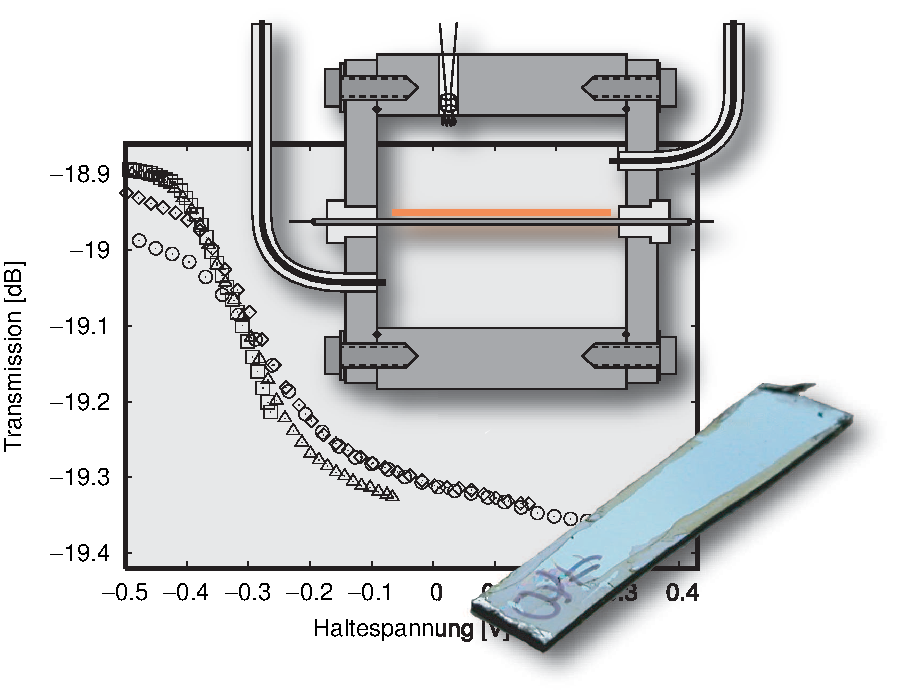
\includegraphics[width=8cm]{titel/titelbild}
\end{center}
\vspace{2ex}
\begin{center}
\LARGE\bfseries Dissertation
\end{center}
\vspace{2ex}
\centerline{zur Erlangung des akademischen Grades}
\centerline{des Doktors der Naturwissenschaften}
\vspace{4ex}
\centerline{an der Universität Konstanz,}
\centerline{Mathematisch-Naturwissenschaftliche Sektion,}
\centerline{Fachbereich Physik}
\vspace{4ex}
%centerline{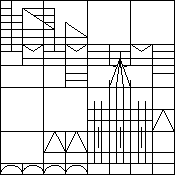
\includegraphics[width=2cm]{titel/unilogo}}
%\vspace{2ex}
\centerline{vorgelegt von}
\vspace{2ex}
\centerline{\bfseries Andreas Würl}
\vspace{5ex}
\centerline{Tag der mündlichen Prüfung: 24.~Juli 2006}
\vspace{0.5ex}
\centerline{\begin{tabular}{l}
Referent: Prof.~Dr.~Paul~Leiderer\\
Referent: Prof.~Dr.~Elke~Scheer
\end{tabular}}
\normalsize
\newpage
\mbox{}\thispagestyle{empty}
\newpage
\setcounter{page}{1}


\pagenumbering{roman}
\tableofcontents

%\pagestyle{empty}
\cleardoublepage
\pagestyle{headings}
\pagenumbering{arabic}
\setcounter{page}{1}
\chapter*{Einleitung}
\addcontentsline{toc}{chapter}{Einleitung}
\markboth{Einleitung}{Einleitung}

Als Sir Joseph John Thomson im Jahre 1897 das Elektron als das erste bekannte Elementarteilchen entdeckte, war dies der Beginn der mittlerweile sehr weit reichenden Elementarteilchenphysik und auch die Grundlage für alle nachfolgenden Entwicklungen in der Elektronik. Viele daraus enstandene Produkte erachten wir mittlerweile in vielen Teilen des täglichen Lebens als selbstverständlich. Als wichtige Meilensteine seien hier die Erfindung der Elektronenröhre für Verstärker und Anzeigeinstrumente, gefolgt von der Entwicklung des ersten Transistors im Jahre 1947 als Geburtsstunde der Halbleiterphysik angeführt. Die schnelle Weiterentwicklung in der Halbleitertechnik führte dann auch zu Halbleiter-Heterostrukturen im so genannten Feldeffekttransistor (FET), der die Stromleitung über die Einschränkung eines zweidimensionalen Ladungskanals von Elektronen durch ein elektrisches Feld steuern kann. 

Wenn aktuell der Begriff eines zweidimensionalen Elektronensystems (2DES) verwendet wird, ist damit in fast allen Fällen die Ausbildung einer zweidimensionalen Elektronenschicht in diesen speziellen Halbleiter"=Schichtstrukturen gemeint. Im Gegensatz dazu weithin unbekannt ist die Möglichkeit, ein freies 2DES oberhalb der Oberfläche von flüssigem Helium zu erzeugen. Dieses "`andere"' 2DES wurde zu Beginn der siebziger Jahre nach einer Idee von \name{W.~Shockley}~\cite{Sho39} unabhängig von \name{M.~W.~Cole} \cite{Col69} und \name{V.~Shikin} \cite{Shi70} vorhergesagt und bald darauf von \name{R.~Williams}, \name{R.~S.~Crandall} und \name{A.~H.~Willis} \cite{Wil71} experimentell bestätigt.

Die Elektronen eines 2DES im Halbleiter können in Grundzügen durch das Modell der Fermi"=Flüssigkeit beschrieben werden, da sich hier die kinetische Energie der Elektronen in derselben Größenordnung wie ihre Coloumb"=Wechselwirkung bewegt und die Elektronendichte sehr hoch ist. Die Fermienergie ist also die für das Verhalten entscheidende Energie. Bei den Elektronen auf flüssigem Helium befindet man sich üblicherweise jedoch in einem völlig anderen Bereich im Phasendiagramm des 2DES. Bei den in diesem System unter experimentellen Bedingungen herrschenden Elektronendichten und Temperaturen ist das Verhältnis der thermischen Energie der Elektronen zu Ihrer kinetischen Energie in der Größenordnung von 1. Im Gegensatz zum 2DES im Halbleiter ist die Elektronendichte hier in einem weiten Bereich einstellbar: Ausgehend von einem Zustand ohne 2DES bei verschwindenden Dichtewerten bis zu einer oberen Grenze bei höheren Elektronendichten, die abhängig von der Erzeugung des Systems auf Bulk"=Helium bei $\unit[2\times10^{13}]{\Em}$ oder auf dünnen Heliumfilmen in einem Bereich von mehr als $\unit[5\times10^{14}]{\Em}$ liegt. Im Halbleiter ist die Elektronendichte in gewissen Bereichen an das Material der Atomrümpfe des Halbleitermaterials gekoppelt und Verbiegungen der Bandstruktur als Einfluss auf die Leitungselektronen sind nur in gewissen Grenzen durchführbar.

Experimente am System Elektronen auf flüssigem Helium werden im Prinzip im Kontext der folgenden zwei Szenarien durchgeführt:
\begin{itemize}
	\item Ein 2DES aus Elektronen auf flüssigem Helium kann als ein {\itshape Modellsystem für ein sehr reines oder verdünntes 2DES} dienen. Da die Elektronendichte im Gegensatz zum Halbleiter beliebig verringert werden kann, ist es möglich, Messungen unter Bedingungen durchzuführen, wie sie dort nur schwer zu erreichen sind. Weiterhin kann man auf Bulk"=Helium bei Temperaturen unter \unit[1]{K} ein sehr reines System mit hochbeweglichen Elektronen erhalten.
	\item In der Literatur finden sich einige Beispiele für die {\itshape Verwendung des 2DES als hochempfindliche Sonde} für die Beschaffenheit der Substrat"= oder der Flüssigkeitsoberfläche. Man kann so mit Hilfe des 2DES z.~B. die Änderung der Oberflächeneigenschaften der Heliumoberfläche~\cite{Kon00} oder aber auch die Eigenschaften der Substratoberfläche unter dem Heliumfilm, wie in Kapitel~\ref{sec:theo_zweikomponenten} dieser Arbeit, charakterisieren.
\end{itemize}

In der vorliegenden Arbeit wurde eine neue Messmethode für das 2DES im Hohlraumresonator entwickelt und etabliert, mit deren Hilfe der Zustand des Systems genauer als bisher untersucht werden kann. Zu Beginn wurden Messungen des 2DES auf Bulk"=Helium durchgeführt, welche sich allgemein durch gut reproduzierbares Verhalten auszeichnen. Im Weiteren wurde auf Elektronensysteme auf dünnen Heliumfilmen übergegangen. Da hier die Präparierung der Substrate für den Heliumfilm eine entscheidende Rolle spielt wurden zuerst einfach herzustellende PMMA"=beschichtete Silizium"=Substrate und später \SiO"=bedeckte Substrate für die Messungen verwendet. Letztere erlauben es, sehr hohe Elektronendichten unter reversiblen Bedingungen zu erreichen. Um die Reproduktion der vorgestellten Verfahren und Vorgehensweisen zu erleichtern wurde eine ausführliche Beschreibung der Vorgehensweisen und Abläufe Wert gelegt. Dies soll sicherstellen, dass die vorgestellten Experimente unter vergleichbaren Bedingungen reproduzierbar sind.

Die Suche nach weiteren Hinweisen auf den Phasenübergang des 2DES in ein entartetes Fermi"=Gas, wie sie schon in \cite{guenzler} und \cite{Gue96} vorgestellt wurden, stellt einen interessanten Aspekt der Arbeit dar. Veröffentlichungen wie \cite{Vos98} zeigen auch das allgemeine Interesse an diesem Thema. Generell ist es so, dass sich die Elektronen eines 2DES im Halbleitersystem normalerweise im  Zustand des entarteten Fermi"=Gases befinden und erst eine geschickte \glqq{}Verdünnung\grqq{} des Systems den Phasenübergang erreichbar macht. Im Falle des 2DES auf flüssigem Helium ist die Vorgehensweise genau entgegengesetzt. Da man diese 2DES von einer verschwindenden Elektronendichte ausgehend erzeugen kann, gilt es hier, besonders hohe Dichten zu erreichen.

Teile der Arbeit sind bereits in folgenden Artikeln veröffentlicht:

\selectlanguage{\english}
\begin{description}
	\item[\cite{Ara99}] {\sc Arai, T.}, {\sc A.~W{\"u}rl}, {\sc P.~Leiderer}, {\sc T.~Shiino}, and\ {\sc K.~Kono}: {\em {C}hemical reaction between hydrogen atoms and electrons on the surface of superfluid {$^4$}{H}e}.\newblock Physica B, {\bf 284--288}, 164, (1999).
0
	\item[\cite{Shi01}] {\sc Shikin, V.}, {\sc J.~Klier}, {\sc I.~Doicescu}, {\sc A.~W{\"u}rl}, and\ {\sc P.~Leiderer}: {\em {D}ip problem of the electron mobility on a thin helium film}. \newblock Phys. Rev. B, {\bf 64}, 73401, (2001).
	
	\item[\cite{Wue01}] {\sc W{\"u}rl, A.}, {\sc J.~Klier}, {\sc P.~Leiderer}, and\ {\sc V.~Shikin}: {\em {E}lectrons on {L}iquid {H}elium in a {R}esonator}. \newblock J. Low Temp. Phys., {\bf }, (2001).
	
	\item[\cite{Kli01}] {\sc Klier, J.}, {\sc T.~G{\"u}nzler}, {\sc A.~W{\"u}rl}, {\sc P.~Leiderer}, {\sc G.~Mistura}, {\sc E.~Teske}, {\sc P.~Wyder}, and\ {\sc V.~Shikin}: {\em {T}wo-{F}raction {E}lectron {S}ystem on a {T}hin {H}elium {F}ilm}. \newblock J. Low Temp. Phys., {\bf 122}, 451, (2001).
	
	\item[\cite{Kli02}] {\sc Klier, J.}, {\sc A.~W{\"u}rl}, {\sc P.~Leiderer}, {\sc G.~Mistura}, and\ {\sc V.~Shikin}: {\em {C}yclotron {R}esonance for 2{D} {E}lectrons on {T}hin {H}elium {F}ilms}. \newblock Phys. Rev. B, {\bf 65}, 165428, (2002).
	
	\item[\cite{Wue03}] {\sc W{\"u}rl, A.}, {\sc J.~Klier}, {\sc P.~Leiderer}, and\ {\sc V.~Shikin}: {\em {C}yclotron {R}esonance for 2{D} electrons on helium films above rough substrates}. \newblock Physica E, {\bf 18}, 184, (2003).
	
	\item[\cite{Kli04}] {\sc Klier, J.}, {\sc A.~W{\"u}rl}, and\ {\sc V.~Shikin}: {\em {A}nticrossing {P}henomena in a {R}esonator with 2{D} {E}lectrons on {L}iquid {H}elium}. \newblock JETP Letters, {\bf 79}, 218, (2004).
\end{description}
\selectlanguage{\ngerman}

\section*{Allgemeine Hinweise}
Da die Erfassung der Messdaten und aller Parameter dieser Arbeit auf rein elektronischem Wege erfolgte, hier noch einige Hinweise, die der Transparenz der vorgestellten Ergebnisse und deren nachträglicher Überprüfbarkeit dienen. 
Abbildungen dieser Arbeit, denen vom Autor gemessene Daten zu Grunde liegen, tragen Vermerke, welcher Abschnitt aus welchen Datensatz dargestellt ist (Nomenklatur <{\itshape Jahr}>/<{\itshape Monat}> \#<{\itshape lfd.\ Nummer}>) und falls zutreffend sind Hinweise auf eine Nachbearbeitung der Originaldaten vermerkt. Die PDF-Version der Arbeit enthält an diesen Stellen noch Verweise auf eine HTML-Seite die einen Überblick über die Daten der jeweiligen Messung und auch die Originaldaten und "=vermerke enthält. Die im Rahmen dieser Arbeit gewonnenen Messdaten können unter \link{www.wuerl.net/diss} jederzeit abgerufen werden.

\chapter{Theoretische Grundlagen}
\label{chap:theo}

\section{Elektronen auf Helium}
Zu Beginn der siebziger Jahre des vorigen Jahrhunderts wurde von \name{M.~W.~Cole} \cite{Col69} und \name{V.~Shikin} \cite{Shi70} unabhängig voneinander die Existenz eines neuen Oberflächenzustands von Elektronen auf der Oberfläche von flüssigem Helium vorgeschlagen. Die Elektronen sind in der Ebene der Flüssigkeitsoberfläche frei beweglich und in der Richtung senkrecht dazu lokalisiert. Sie befinden sich dann in Zuständen, die den Zuständen des Elektrons im Wasserstoffatom sehr ähnlich sind.
Allerdings besitzen diese Zustände -- aufgrund der hier sehr viel schwächeren Bindung, die nur aus der Coulombkraft mit der Bildladung des Elektrons im Helium resultiert -- eine deutlich größere Bindungslänge und eine stark reduzierte Bindungsenergie.

Wenig später wurde ein Experiment  von \name{R.~Williams}, \name{R.~S.~Crandall} und \name{A.~H.~Willis} \cite{Wil71} durchgeführt, in dem die Lebensdauer eines solchen vorhergesagten Oberflächenzustandes unter verschiedenen äußeren Bedingungen untersucht wurde. \name{Williams} \ea{} haben eine Oberfläche flüssigen Heliums von der Gasseite her mit Elektronen beladen und konnten eine korrelierte Verringerung des elektrischen Feldes über der Heliumoberfläche messen. Durch kurzzeitiges Abschalten der positiven Spannung der die Elektronen anziehenden Halteelektrode im flüssigen Helium konnten sie so das Verschwinden der Elektronen des 2DES in den Gasraum hinein detektieren und somit die Lebensdauer dieses Zustandes ohne angelegte Haltespannung bestimmen.

Ein Experiment zur lateralen Beweglichkeit der Elektronen im 2DES -- also eine erste Transportmessung am 2DES -- wurde von \name{W.~T.~Sommer} und \name{D.~J.~Tanner} \cite{Som71} durchgeführt. Hierbei wurde die Beweglichkeit der Elektronen im 2DES über ihren Einfluss auf das elektrische Übersprechen zwischen zwei in einer Ebene unter dem flüssigen Helium liegenden Kondensatorplatten bestimmt.

\subsection{Das Potential der Elektronen im 2DES}
Im Jahre 1974 wurde dann von \name{C.~C.~Grimes} und \name{T.~R.~Brown} \cite{Gri74} ein direkter Beweis des Vorhandenseins der Oberflächenzustände der Elektronen vorgestellt. Die Energieniveaus der lokalisierten Elektronen wurden durch ihre  Absorption von Mikrowellen bei einer Frequenz in der Größenordnung von \unit[100]{GHz} nachgewiesen. Hier erhält man Absorptionslinien für die Übergänge $1\rightarrow2$ und $2\rightarrow3$, deren Energien charakteristisch für das schwach gebundene Elektronensystem auf flüssigem Helium sind.
Die Struktur des Potentials, in dem sich ein Elektron auf Bulk-Helium bewegt, konnte genauer überprüft werden. Dieses ist aus zwei Anteilen zusammengesetzt und entsteht alleine durch die Anwesenheit eines Elektrons selbst:

\begin{enumerate}
    \item In den oberen Halbraum hinein reicht ein schwaches, attraktives Coulomb"=Potential, das von der Bildladung erzeugt wird, die das Elektron im Dielektrikum Helium induziert.
    \item In der Nähe der Heliumoberfläche gibt es eine Barriere von etwa \unit[1]{eV}, die das Elektron überwinden muss, um in das flüssige Helium eindringen zu können. Diese Barriere ergibt sich aufgrund der Pauli-Abstoßung, die das Elektron durch die Anwesenheit der beiden $1s$-Elektronen der Heliumatome erfährt.

Da die Barriere mit ungefähr \unit[1]{eV} viel höher als die Tiefe des anziehenden Coulomb-Potentials von einigen meV ist, wird sie für Berechnungen der Wellenfunktion, Energie, etc.\ näherungsweise als unendlich hohe Barriere angenommen.
\end{enumerate}

\begin{figure}[h!tbp]
    \centerline{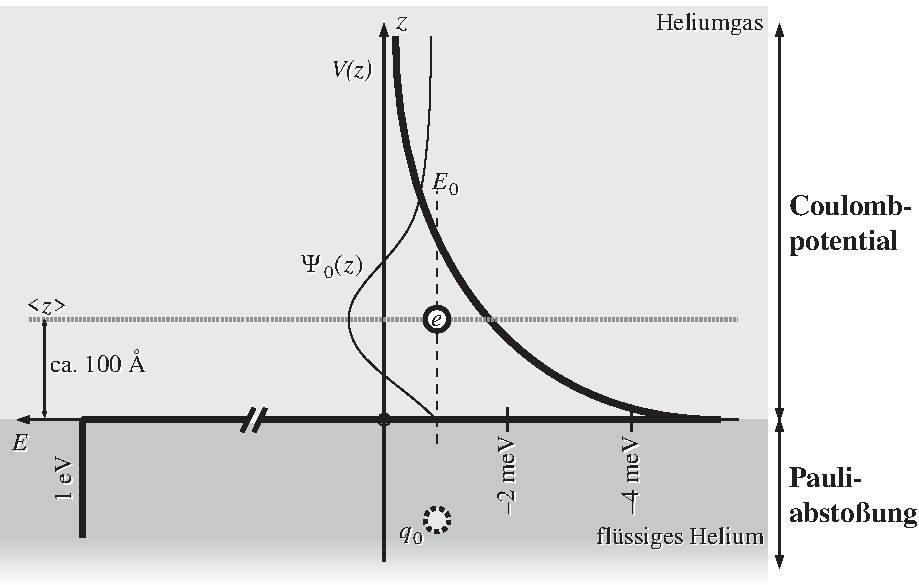
\includegraphics[width=\bigwidth]{theo_electrons_on_helium/SSE}}
    \caption[Das Potential, in dem sich ein Elektron auf flüssigem Helium bewegt.]{Das Potential, in dem sich ein Elektron auf flüssigem Helium bewegt. Am rechten Rand ist angezeigt, welcher Teil des Potentials für ein Elektron im jeweiligen Bereich dominiert.} 
    \label{fig:potential}
\end{figure}
Wenn man beide Anteile zu einem Gesamtpotential zusammenführt, das in Abbildung~\ref{fig:potential} schematisch dargestellt ist, erhält man folgenden Ausdruck:
    \begin{equation}
        \label{eqn:SSE_Potential}
        V(z)=\left\{\begin{array}{cl}
             V_0 & \;z\leq0\\
            -\frac{1}{4\pi\,\epsilon_0}\frac{q_0\,e^2}{z+\beta} & \;z>0\\
        \end{array}\right.
        \quad\textrm{mit}\quad
        \begin{array}{rl}
            V_0=&\unit[1]{eV}\\
            q_0=&\frac{\epsilon-1}{4(\epsilon+1)}\\
        \end{array}\quad.
    \end{equation}

Hierbei ist $q_0$ die Bildladung, deren Größe durch die \DK\ des Heliums bestimmt wird. Auf dünnen Heliumfilmen kommt noch die weit höhere Bildladung im Substrat hinzu. Der Offset $\beta$ ergibt sich nach \name{Grimes} \ea~\cite{Gri74} aus der physikalischen Tatsache, dass die Ebene, in der die Pauli-Abstoßung einsetzt durch die Überlappung der Wellenfunktionen der $1s$-Elektronen des Heliums mit der Wellenfunktion der 2D-Elektronen gegeben ist. Die Symmetrieebene der Bildladungen ist um ungefähr einen Atomradius dazu versetzt und verhindert für $\beta>0$ die Singularität des Potentials im $z$"=Koordinatenursprung. \name{Grimes} \ea\  bestimmten für $\beta$ etwa \unit[1]{\AA}, was näherungsweise mit dem Radius der Helium"=Atome übereinstimmt.

Die Lösung des Problems mit dem Potential aus Gleichung~\eqref{eqn:SSE_Potential} ist, bis auf die hier nicht vorhandene Kugelsymmetrie des Systems, identisch zur bekannten Lösung der Schrödingergleichung des Elektrons im Wasserstoffatom. Für den Bohrschen Radius ergibt sich hier aufgrund der im Vergleich zum Wasserstoffatom wesentlich schwächeren Bindung des Elektrons eine Länge von ca.\ \unit[114]{ \AA} (vgl. H-Atom \unit[0.5]{\AA}) und eine Grundzustandsenergie von $\unit[-0.65]{meV}$ (H-Atom $\unit[-13.6]{eV}$). Der Energieabstand zum ersten angeregten Zustand beträgt \unit[0.49]{meV}, was einer Temperatur von \unit[5.7]{K} entspricht; dies bedeutet, dass sich bei Temperaturen um \unit[1.5]{K} näherungsweise alle Elektronen im Grundzustand befinden und somit ein rein zweidimensionales Elektronensystem vorliegt.

Im Experiment wird üblicherweise eine definierte Haltespannung an das Substrat angelegt, um eine direkt davon abhängige Elektronendichte im 2DES zu erhalten (diese Abhängigkeit wird im Abschnitt~\ref{ssec:e_density} genauer untersucht). In diesem Fall eines zusätzlichen konstanten externen elektrischen Feldes in Richtung der $z$-Achse erhält das  Potential~\eqref{eqn:SSE_Potential} einen weiteren Term, der das durch das zusätzliche statische elektrische Feld $E_\perp$ erzeugte linear mit $z$ skalierende Potential berücksichtigt:
	\begin{equation}
			\label{eqn:clamping_potential}
			e E_\perp z\quad.
	\end{equation}
Dieser Term für das externe elektrische Feld hat zur Folge, dass die Schrödingergleichung für das Problem nicht mehr analytisch lösbar ist. Wenn man ihre Lösung jedoch näherungsweise bestimmt, bewirkt das zusätzliche Feld bei einer Erhöhung eine Verschiebung und Spreizung der erhaltenen Energieniveaus, wie auch vom Stark"=Effekt bekannt. 

\subsection{Stabilität von Elektronen auf Bulk"=Helium}
\label{ssec:bulk_stabilitaet}

Falls sich ein 2DES auf der Oberfläche von Bulk"=Helium befindet, wird die Dispersionsrelation der Oberflächenwellen (Ripplonen) auf einer He"=Schicht der Dicke $d$ durch den zusätzlichen elektrostatischen Druck, den die Elektronen auf die Flüssigkeitsoberfläche ausüben, folgendermaßen modifiziert:
\begin{equation}
    \label{eqn:ripplon_dispersion_bulk}
        \omega^2_\text{ripplon}=\frac{\rho_\text{s}}{\rho_\text{He}}\left[g k_\text{ripplon}+
            \frac{\sigma_\text{lv}}{\rho_\text{He}} k^3_\text{ripplon}-\frac{4\pi n^2e^2}{\rho_\text{He}} k^2_\text{ripplon}F(k_\text{ripplon},\varepsilon)\right]\tanh(k_\text{ripplon} d)\quad.
\end{equation}
Hierbei ist $g$ die Erdbeschleunigung, $\sigma_\text{lv}$ die Oberflächenspannung, $\rho_\text{He}$ die Dichte des flüssigen Heliums, $n\,e$ ist die Ladungsdichte des 2DES und $\frac{\rho_s}{\rho_\text{He}}$ der suprafluide Anteil im Helium.

Wenn man die Elektronendichte immer weiter erhöht, erhält man für $n_{s,\text{crit}}\approx\unit[2\times10^{13}]{\Em}$ \cite{Gor73,Mim78,Wan79,Ebn80,Wil82} die elektrohydrodynamische (EHD) Instabilität. Hierbei verhält sich das System wie die instabile Schichtung einer schwereren Flüssigkeit über einer leichteren. Sobald an einer Stelle die Grenzfläche der Flüssigkeit aus der labilen Anfangsposition ausgelenkt wird, überwiegen die Kräfte, die diese Auslenkung unterstützen über die Rückstellkräfte; das System wird folglich instabil. In Abbildung~\ref{fig:bulk_instability} kann man am Beispiel von positiv geladenen Ionen an einer $^3$He"=$^4$He"=Grenzfläche sehen, dass eine Erhöhung der Elektronendichte in der Ripplonendispersionsrelation~\eqref{eqn:ripplon_dispersion_bulk} ab einer bestimmten kritischen Dichte $n_\text{crit}$ zu einer "`Aufweichung"' der Ripplonenmode führt. Ab der oberen Grenze $n_{s,\text{crit}}$ der erreichbaren Ladungsdichte wird die Ripplonenfrequenz $\omega$ in der Dispersionsrelation gleich 0, was das Einsetzen der Instabilität bedeutet. Für Ladungsdichten größer als $n_{s,\text{crit}}$ kann die Heliumoberfläche eine Auslenkung aus dem Gleichgewicht nicht mehr mit Hilfe der Oberflächenspannung und der Gravitation ausgleichen. Für Elektronen auf flüssigem Helium bedeutet das, dass eine Blase von Elektronen in das flüssige Helium hineingezogen wird. Dieser Vorgang wird als Durchbrechen der Elektronen bezeichnet.

\begin{figure}[h!tbp]
    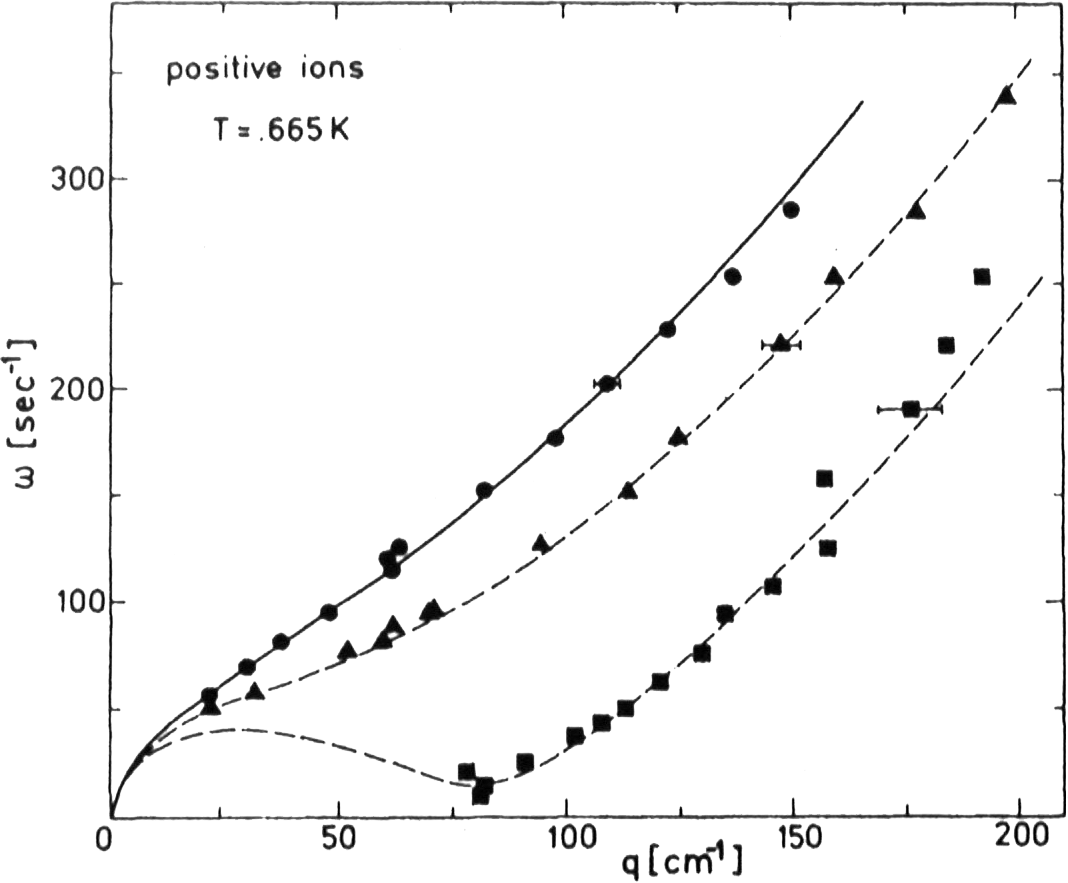
\includegraphics[width=\smallwidth]{theo_electrons_on_helium/instability}\hfill
    \begin{minipage}[b]{\textwidth-\smallwidth-2\tabcolsep}
        \caption[Ripplonendispersionsrelation an der Grenzfläche einer gesättigten $^3$He"=$^4$He"=Mischung]{Ripplonendispersionsrelation an der Grenzfläche einer gesättigten $^3$He"=$^4$He"=Mischung nach \name{Leiderer} \cite{Lei79}. Die Grenzfläche ist von unten mit positiven Ionen beladen.\par$T=\unit[0.665]{K}$, $n_c=\unit[4.8\times10^{12}]{\Em}$, $E_c=\unitfrac[87.5]{kV}{m}$. $E/E_c=0.12$ ({\large$\bullet$}), 0.71 ($\blacktriangle$) und 0.995 ({\tiny$\blacksquare$}).}
        \label{fig:bulk_instability}
    \end{minipage}
\end{figure}

Für ungesättigte Elektronendichten, $n<n_{s,\text{crit}}$, d.~h.\ für geringere Elektronendichten aber höhere Haltespannungen, kann ebenfalls ein so hoher Elektronendruck erreicht werden, der auch in diesem Fall zu einer Instabilität und somit zum Einbrechen von Elektronen in das Bulk"=Helium führen kann.

Das Auftreten der elektrohydrodynamischen Instabilität kann bei Messungen von 2DES auf Bulk"=Helium auch als Eichpunkt für die Elektronendichte herangezogen werden. Dies wird später z.\ B.\ bei der Bestimmung der Elektronenproduktion der Filamente in Abschnitt~\ref{ssec:electron_production} und zur Eichung des Kondensators zur Bestimmung der Helium"=Füllhöhe in \ref{ssec:level_calib} Verwendung finden.

\begin{figure}[h!tbp]
    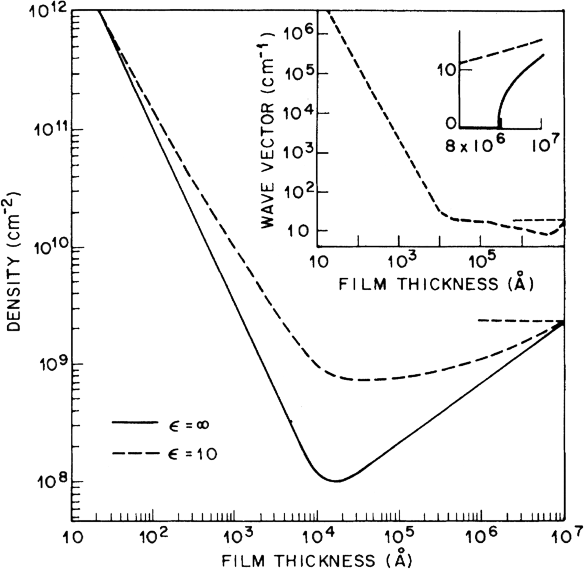
\includegraphics[width=\smallwidth]{theo_electrons_on_helium/stability}\hfill
    \begin{minipage}[b]{\textwidth-\smallwidth-2\tabcolsep}
        \caption[Kritische Elektronendichten der elektrohydrodynamischen Instabilität.]{Abhängigkeit der kritischen Elektronendichte der elektrohydrodynamischen Instabilität nach \name{F. Peeters} \cite{Pee84} von der Dicke der Heliumschicht zwischen Substrat und 2DES für ein metallisches (durchgezogene Linie) und ein nicht"=metallisches Substrat. Im Einsatz ist die Wellenzahl aufgetragen, an der die Instabilität zuerst auftritt (vgl.\ hierzu Abb.~\ref{fig:bulk_instability}).}
        \label{fig:bulk_instability_dep}
    \end{minipage}
\end{figure}

Um die Beschränkung der maximal erreichbaren Elektronendichte zu umgehen, kann man, wie bereits in \cite{Ike81}, \cite{Mon82} und \cite{Wil82} vorgeschlagen, zu gesättigten Heliumfilmen als Unterlage für die Elektronen übergehen. Hier wird die Ripplonendispersionsrelation \eqref{eqn:ripplon_dispersion:film} durch die starke van"=der"=Waals"=Wechselwirkung zwischen den Heliumatomen und dem darunter liegendem Substrat derart modifiziert, dass die Erhöhung der Elektronendichte nicht zu einer Instabilität führt. Dies wird später in Abschnitt~\ref{ssec:film_stability} genauer untersucht.

\subsection{Die Beweglichkeit der Elektronen im 2DES}
\label{ssec:mobility}
Ohne äußeres elektrisches Feld ist die Geschwindigkeit der Elektronen $\vec v$ im Mittel gleich Null. Bei Anwesenheit eines elektrischen Feldes werden die Elektronen beschleunigt. Stellt man sich ein Elektron zur Zeit $t=0$ vor, dann ist $t$ die Zeit, die seit der letzten Kollision vergangen ist. Ein äußeres Feld ändert die Geschwindigkeit um $-e\vec E\frac{t}{m}$, was sich aus
    \begin{equation}
        F=m_ea\quad\Rightarrow\quad a=\frac{F}{m_e}\quad\Rightarrow\quad v=at=\frac{Ft}{m_e}
    \end{equation}
ergibt. Die durchschnittliche Geschwindigkeit $\vec v_\text{avg}$ und die Beweglichkeit $\mu$ der Elektronen wird bestimmt durch die mittlere Streuzeit $\tau$:
    \begin{equation}
        \vec v_\text{avg}=-\frac{e\vec E\tau}{m_e}\ttextt{und}		\mu=\frac{e\,\tau}{m_e}\quad.
    \end{equation}

Eingesetzt in die Gleichung für die Stromdichte $j=n e \vec v$ ergibt sich das Drude"=Gesetz für die Gleichstromleitung in einem metallischen Leiter:
	$\vec j = \sigma\vec E$ mit der Leitfähigkeit $\sigma$: $\sigma=n e \mu$.

\subsection{Elektronen im elektrischen Wechselfeld}
\label{ssec:eqns_of_motion}
Aus der klassischen Bewegungsgleichung eines einzelnen Elektrons im elektrischen Feld $\vec E$ mit einem Lokalisierungspotential der Frequenz $\omega_0$ und einer mittleren Stoßzeit $\tau$, 
\begin{equation}
		m\ddot{\vec x}+\frac{m}{\tau}\dot{\vec x}+m\omega_0^2\vec x=e\vec E
\end{equation}
kann man über einen harmonischen Lösungsansatz $\vec x, \vec E\propto e^{i\omega t}$ aus dem Realteil der Lösung für die Geschwindigkeit $\vec v$ des Elektrons, die Dissipation $P$ des Elektronensystems bestimmen:
\begin{equation}
	P=\frac{m}{\tau}\vec v\vec v^*=\frac{Ne^2}{m}\tau\frac{1}{1+\left(\frac{\omega_0^2-\omega^2}{\omega}\right)^2\tau^2}E^2\quad.
\end{equation}

Aus dem Realteil der Ortsfunktion $\vec x$ läßt sich über das Gesamtdipolmoment der Elektronen $\vec P=N\vec p=N\,e\,\vec x$ analog die Suszeptibilität des Elektronensystems bestimmen:
\begin{equation}
\chi=\frac{\left|\vec P\right|}{\varepsilon_0E}=\frac{Ne^2}{m}\tau^2\frac{(\omega_0^2-\omega^2)\tau^2}{\left(\omega_0^2-\omega^2\right)^2\tau^4+\omega^2\tau^2}\quad.
\end{equation}

\subsection{Wichtige Streumechanismen}
\label{ssec:scattering}

\begin{figure}[h!tp]
	\hfill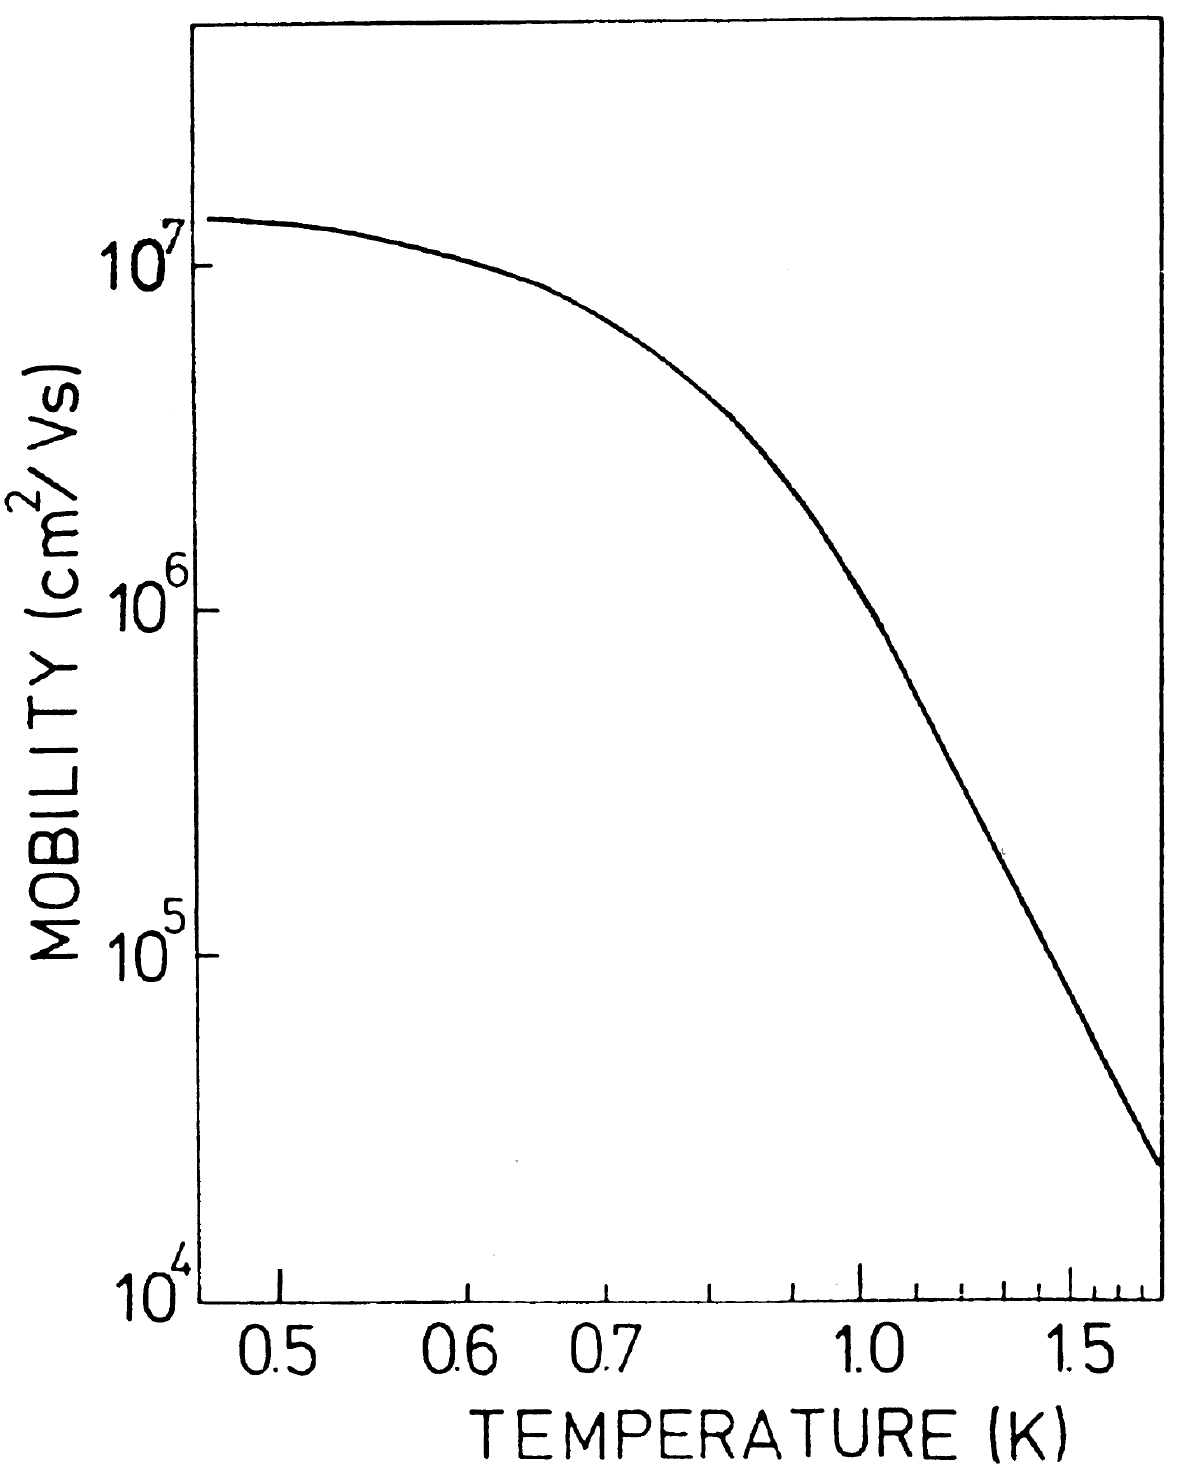
\includegraphics[width=2in]{theo_electrons_on_helium/mobility}\hfill
	\begin{minipage}[b]{\textwidth-\smallwidth-2\tabcolsep}
		\caption[Temperaturabhängigkeit der Beweglichkeit von Elektronen auf Bulk"=Helium]{Messung der Beweglichkeit von Elektronen auf Bulk"=Helium aus \cite{Lei92}. Deutlich sieht man die im Text beschriebene exponentielle Temperaturabhängigkeit im Regime der Gasatomstreuung oberhalb von ca.\ \unit[0.8]{K} und die schwache Temperaturabhängigkeit im Regime der Streuung an Ripplonen unterhalb von ca.\ \unit[0.7]{K}.\label{fig:mobility}}
	\end{minipage}
\end{figure}

Die Elektronen über der Oberfläche von flüssigem Helium werden auf Grund von verschiedenen Mechanismen gestreut. Oberhalb von ca.\ \unit[0.8]{K} dominiert die Streuung an den Helium"=Gasatomen, die mit der Temperatur exponentiell zunimmt. Dies wurde von \name{Sommer} \ea \cite{Som71} experimentell nachgewiesen. Unterhalb von \unit[0.7]{K} ist nur noch die Streuung an den Ripplonen der Heliumoberfläche dominierend -- experimenteller Nachweis durch \name{Grimes} \ea \cite{Gri76} -- die allerdings auf Grund der schwachen Temperaturabhängigkeit der Anregung von Ripplonen die Beweglichkeit der Elektronen kaum beeinflusst (siehe auch \cite{Bri77,Col74}). Auf dünnen Heliumfilmen bestehen auf Grund der Rauigkeit des Substrats viele Streuzentren, die dann die Beweglichkeit der Elektronen um einige Größenordnungen reduzieren. 

\section{Phasendiagramm eines 2DES}
\label{sec:theo_phasendiagramm}

Das Phasendiagramm eines 2DES auf flüssigem Helium wird bestimmt durch das Wechselspiel folgender Energien:
\begin{itemize}
	\item thermische Energie $E_\text{therm}=k_\text{B}T \propto T\quad$\phantom{$\frac{\hbar^2}{\epsilon_0}$}
	\item Coulomb"=Energie $E_\text{Coulomb}=\frac1{4\pi\epsilon_0} e^2\sqrt{\pi n} \propto \sqrt{n}\quad$\phantom{$\frac{\hbar^2}{\epsilon_0}$}
	\item Fermi"=Energie $E_\text{F}=\frac{\pi\hbar^2}{m_e}n\propto n$
\end{itemize}
Diese sind abhängig von den thermodynamischen Parametern des Systems. Wie aus obiger Aufstellung ersichtlich ist, sind dies die Elektronendichte $n_s$ und die Temperatur $T$ des Elektronensystems. $n_s$ und $T$ sind die im Phasendiagramm interessanten Achsen; zusätzlich sind das Magnetfeld $B$ und auf dünnen Heliumfilmen die Polarisierbarkeit des Substrats weitere Parameter, die das Phasenverhalten des 2DES modifizieren. Diese können als weitere Achsen des Phasendiagramms dienen.

Bei typischen Elektronendichten von $10^{9}$ bis $\unit[10^{13}]{\Em}$ verhalten sich die Elektronen klassisch, da die Fermi"=Energie im Bereich von $0.003$ bis $\unit[30]{mK}$ liegt. Das bedeutet, dass die Fermi"=Energie bei Experimenten mit 2DES auf Bulk"=Helium im hier erreichbaren Temperaturbereich keine Rolle spielt. Deshalb ist hier das Verhältnis der Größen der thermischen Energie und der Coulomb"=Energie wichtig. Dies kann zum Phasenübergang vom klassischen Elektronengas zum Elektronenfestkörper, dem so genannten Wigner-Kristall führen. Dieses Phänomen wurde theoretisch von \name{E.~Wigner} \cite{Wig34} vorhergesagt.

Wenn man in der Lage ist, wie für Elektronen auf dünnen Heliumfilmen theoretisch vorhergesagt, die Elektronendichten in Bereiche bis zu \unit[10$^{16}$]{\Em}  zu erhöhen, dann wird das Verhältnis von Fermienergie und Coulomb"=Energie bestimmend für den Zustand des Systems. Man nähert sich einem weiteren Phasenübergang vom Wigner"=Kristall zum Zustand des entarteten Fermi-Gases von Elektronen, welcher schon aus der Physik von Elektronen in Halbleitern und Metallen bekannt ist.

\subsection{Übergang zum Elektronenfestkörper nach \name{Wigner}}

Wie \name{E.~Wigner} bereits in \cite{Wig34} bei der Untersuchung der Wechselwirkung von Elektronen in Metallen festgestellt hat, können die Elektronen mit einer kompensierenden positiven Ladung im Hintergrund und bei geringer kinetischer Energie in drei Dimensionen einen $bcc$-Kristall bilden. Dies passiert, obwohl ihre Wechselwirkung durch die Coulomb-Kräfte rein abstoßend ist. Einen solchen Übergang kann man auch in zwei Dimensionen beobachten, was von \name{R.~Crandall} \ea{} \cite{Cra71} für das System von Elektronen auf Helium und von \name{A.~Chaplik} \ea{} \cite{Cha72} für Elektronen oder Löcher in Halbleiter-Inversionsschichten vorgeschlagen wurde. Der erste experimentelle Nachweis dieses Phasenübergangs bei Elektronen auf Bulk"=Helium gelang \name{Grimes} und \name{Adams} \cite{Gri79}.

Den Phasenübergang von der klassischen Elektronenflüssigkeit zum Elektronenfestkörper erwartet man, wenn die potentielle Energie $\brak{V}$ der Elektronen über ihre thermische Energie $\brak{K}$ dominiert. Der Parameter $\Gamma$ steht für das Verhältnis dieser beiden Größen und charakterisiert das thermodynamische Verhalten des Systems bezüglich des Phasenübergangs:
    \begin{equation}
        \label{eqn:tph_VWRatio}
        \frac{\brak{V}}{\brak{K}} \equiv \Gamma\quad.
    \end{equation}
Für ein klassisches 2DES ist
	\begin{equation}
		\label{eqn:Gamma_klass}
		\Gamma=\frac1{4\pi\epsilon_0}\frac{e^2\sqrt{\pi n}}{\kB T}\quad.
	\end{equation}
Der Wert von $\Gamma$ bestimmt das thermodynamische Verhalten des 2DES im Bezug auf die Wigner-Kristallisation:
\begin{description}
	\item[$\Gamma\lesssim1$:] In diesem Bereich dominiert die kinetische Energie der Elektronen. Es liegt ein klassisches Elektronengas vor. Die Fermi-Energie ist bei den üblichen Elektronendichten im Bereich einiger Millikelvin und spielt daher hier keine Rolle.
	\item[$1\lesssim\Gamma\lesssim100$:] In diesem Bereich wird die Elektronenbewegung hochkorreliert, allerdings findet noch keine Kristallisation statt.
	\item[$\Gamma\gtrsim100$:] Hier dominiert die potentielle Energie. Man erwartet einen Phasenübergang, nach dem die Elektronen in einem periodischem Gitter angeordnet sind.
\end{description}

Der Phasenübergang vom Wigner"=Kristall zur klassischen Elektronenflüssigkeit  wird von der \mbox{KTHNY}\footnote{Kosterlitz und Thouless \cite{Kos73}, Nelson und Halperin \cite{Nel79} und Young \cite{You79}}-Theorie gut beschrieben. Diese Theorie beinhaltet, dass der Vorgang des Schmelzens durch das Aufbrechen vorher gebundener Paare von Versetzungen im Kristallgitter initiiert wird.

Eine molekulardynamische Simulation von \name{R. Morf} \cite{Mor79} auf Basis der KTHNY"=Theorie ergab einen Bereich von $125<\Gamma<132$. Für ein 2DES auf dünnen Heliumfilmen bestimmten \name{F.~Peeters} \ea{} \cite{Pee83} mit Hilfe numerischer Simulationen und einem Wert von $\Gamma(d=\infty)=137$ das in Abbildung~\ref{fig:phase_diag_scheme} zu sehende Phasendiagramm für Elektronen auf Bulk"=Helium und dünnen Heliumfilmen auf metallischen und dielektrischen Substraten. 

\begin{figure}[h!tbp]
	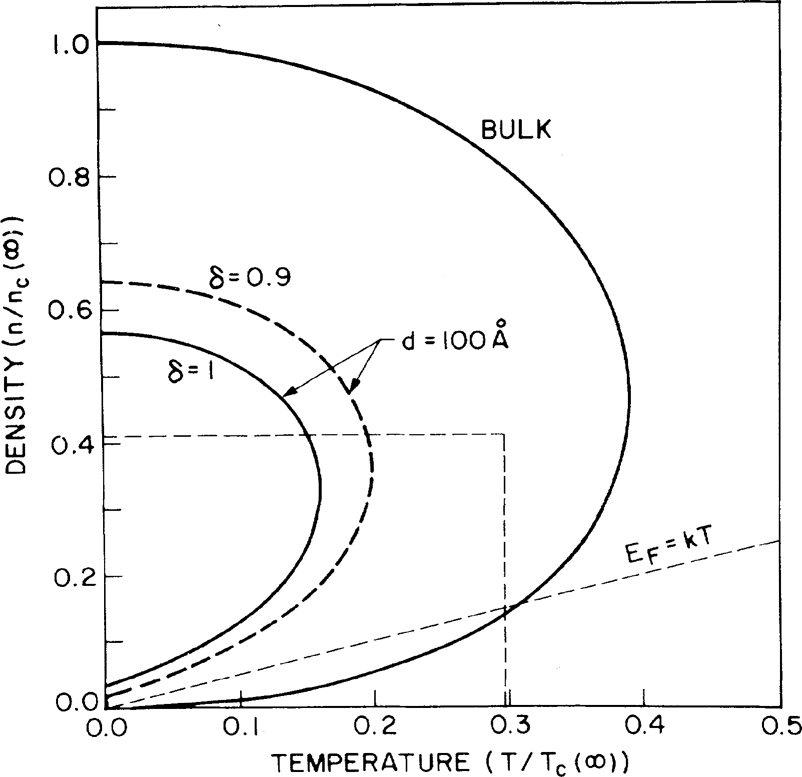
\includegraphics[width=\smallwidth]{theo_phasendiagramm/Pee83_PD}%
	\hfill%
	\begin{minipage}[b]{\textwidth-\smallwidth-\tabcolsep}
	\caption[Schematisches Phasendiagramm des 2DES.]{Schematisches Phasendiagramm des 2DES nach \cite{Pee83}. Zusätzlich zur Phasengrenze auf Bulk"=Helium ist hier noch der Verlauf auf einem \unit[10]{nm} dünnen Heliumfilm auf Saphir ($\delta=0.9$) und metallischem Substrat ($\delta=1$) angezeigt.\par$n_c=\unit[2.4\times10^{16}]{\Em}$ und $T_c=\unit[33]{K}$.}
	\label{fig:phase_diag_scheme}
	\end{minipage}
\end{figure}

\subsubsection{Phasendiagramm auf dünnen Heliumfilmen}
\label{ssec:phasediag_films}
Weil auf dünnen Heliumfilmen der Charakter der Elektron"=Elektron ($e$-$e$) Wechselwirkung stark von der Elektronendichte und der Helium-Filmdicke abhängig ist, bleibt auch das Phasendiagramm des 2DES davon nicht unberührt. In Abbildung~\ref{fig:phase_diag_scheme} sieht man, dass der Bereich des Wigner"=Kristalls im Phasendiagramm auf dünnen Heliumfilmen dadurch deutlich reduziert wird. Maximal wird dieser Effekt für ein metallisches Substrat ($\delta=1$).
\enlargethispage{2ex}

Nach den analytischen Rechnungen von \name{M.~Saitoh} \cite{Sai89} und dem Vergleich mit Messungen von \name{A.~Dahm} wurde für $\Gamma(d)\approx137$ auf dünnen Heliumfilmen ein ähnlicher Wert wie für Bulk"=Helium bestimmt. Nach \name{Saitoh} gilt für die Schmelztemperatur $T_m(d)$ näherungsweise
\begin{equation}
	\label{eqn:wc_melting_temp}
	k_BT_m(d)=\frac1{4\pi\epsilon_0}\frac{e^2\sqrt{\pi n}f(d)}{\Gamma(d)}\ttextt{mit}
	f(d)=1-\delta\left(1+4\pi n \frac{d^2}{c_0^2}\right)^{-\frac32}\quad.
\end{equation}
Hierbei ist $\delta=(\epsilon_{r,\text{Substrat}}-1)/(\epsilon_{r,\text{Substrat}}+1)$ und $c_0=1.1061$ eine Konstante. Diese Formel wird später im Abschnitt~\ref{ssec:wigner_auswertung} bei der Berechnung der $\Gamma$-Werte der Phasenübergänge Verwendung finden.

\subsection{Übergang vom Elektronenfestkörper zum entarteten Fermi"=Gas}
Beim Übergang vom Elektronenfestkörper zum entarteten Fermi"=Gas ist es das Wechselspiel zwischen Coulomb"=Energie und Fermi"=Energie, das den Phasenübergang bestimmt:
\begin{equation}
	\label{eqn:qm_Gamma}
	\Gamma_\text{QM}=\frac{E_\text{Coulomb}}{E_\text{Fermi}}
		=\frac{m_e e^2}{4\pi\epsilon_0\hbar^2 \sqrt{\pi}}\frac1{\sqrt{n}}\quad.
\end{equation}
Die Ordnung des 2DES im Wigner"=Kristall, hervorgerufen durch die über die thermische Energie des Systems dominierende Coulombenergie, wird aufgrund der bei hohen Elektronendichten starken Einschränkung der Elektronen im Ortsraum wieder zerstört. Aufgrund der Heisenbergschen Unschärferelation nehmen dann die Fluktuationen der Elektronen im Impulsraum stark zu. Dies hat zur Folge, dass der Wigner"=Kristall schmilzt und man ein entartetes Fermi"=Gas erhält.


\section{2DES auf gesättigten Heliumfilmen}
Wenn man in den Bereich des Phasendiagramms des 2DES vorstoßen will, in dem das 2DES als entartetes Elektronengas vorliegt, muss man Elektronendichten von $\gtrsim\unit[10^{15}]{\Em}$ erreichen. Derart hohe Elektronendichten sind, wie im vorigen Kapitel beschrieben auf Bulk"=Helium nicht stabil zu halten. Wenn man nun, wie schon in \cite{Ike81} vorgeschlagen, auf dünne Heliumfilme übergeht, kommt zusätzlich zur Stabilisierung durch die Gravitation die bei dünnen Filmen viel stärkere van"=der"=Waals"=Kraft zum tragen. In diesem Abschnitt sollen die Eigenschaften von Elektronen auf dünnen Heliumfilmen nun genauer untersucht werden.
 
\subsection{Allgemeine Eigenschaften}
\label{ssec:hefilm_allgemein}

\begin{figure}[h!tbp]
    \begin{center}
        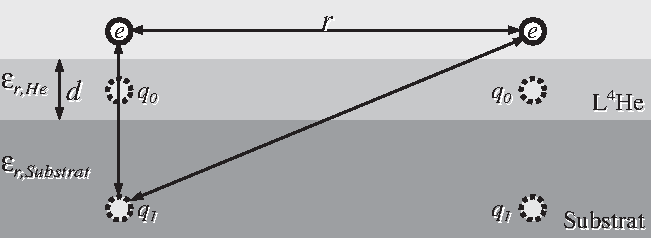
\includegraphics{theo_helium_filme/e_auf_filmen}
    \end{center}
    \caption[Wechselwirkungen auf dünnen Heliumfilmen]{Elektronen auf dünnen Heliumfilmen. Gezeigt ist schematisch wie die Wechselwirkung zwischen den Elektronen und den Bildladungen im Heliumfilm und Substrat zustande kommt. Der Charakter der $e$"=$e$"=Wechselwirkung wird durch die Abstände $d$ und $r$ bestimmt. Für $r\gg d$ ist die Wechselwirkung dipolartig, für $r\lesssim d$ Coulomb"=artig.}
    \label{eqn:film_schema}
\end{figure}

Der Übergang von 2DES auf Bulk"=Helium zu 2DES auf dünnen Heliumfilmen wird begleitet von der Änderung einiger Eigenschaften des Systems:

\begin{itemize}
    \item Der Heliumfilm ist aufgrund der starken van"=der"=Waals"=Wechselwirkung der Heliumatome mit dem Substrat stabil gegenüber der Aufweichung der Ripplonenmoden -- ganz im Gegensatz zur Oberfläche des Bulk"=Heliums. Die von dort bekannte elektrohydrodynamische Instabilität tritt hier nicht auf und als Folge davon kann der Heliumfilm weit höhere Elektronendichten tragen. Ob es hier eine obere Grenze für die Elektronendichte gibt, wurde in der Literatur \cite{Ike81,Etz84,Hu90} bereits diskutiert und wird in Abschnitt~\ref{ssec:film_stability} vorgestellt.
    \item Durch die im Vergleich zu Bulk"=Helium größere Dielektrizitätskonstante des Substrates folgt eine daraus resultierende stärkere Bildladung, so dass sich der coulombartige Charakter (hier $V\propto \frac1r$) der $e$-$e$"=Wechselwirkung für $r\gg d$ zunehmend in einen dipolartigen Charakter (mit $V\propto\frac1{r^3}$) wandelt. Dadurch wird die $e$-$e$-Wechselwirkung abgeschwächt, was zur Folge hat, dass das in Kapitel~\ref{sec:theo_phasendiagramm} vorgestellte Phasendiagramm eines 2DES modifiziert wird. Aufgrund der reduzierten $e$-$e$-Wechselwirkungsenergie verschiebt sich der Phasenübergang von der klassischen Elektronenflüssigkeit in den Wigner-Kristall zu höheren Elektronendichten hin. Der Quanten-Phasenübergang, der bei hohen Elektronendichten stattfindet, tritt bei kleineren Elektronendichten auf. Insgesamt schrumpft also der Bereich im Phasendiagramm, in dem ein Wigner-Kristall vorliegt. In Abbildung~\ref{fig:phase_diag_scheme} kann man das Phasendiagram von Bulk"=Helium mit dem von einem dünnen Heliumfilm auf Saphir und einem metallischen Substrat sehen. 
    \item Die Bindung der Elektronen an die Heliumoberfläche wird aufgrund der größeren Bildladung im dielektrischen Substrat stärker. Dies hat zur Folge, dass sich die Energieniveaus der Elektronen im 2DES zu tieferen Energien hin verschieben und sich der Abstand der Niveaus vergrößert.
    \item Bei dünnen Heliumfilmen muss zusätzlich auch der Einfluss der Oberflächenrauigkeit des Substrats berücksichtigt werden. Diese ist von Bedeutung, da alle im Experiment verwendeten Substrate eine Restrauigkeit besitzen. Man kann nicht mehr davon ausgehen, dass alle Elektronen frei sind, wie im sehr reinen System Elektronen auf Bulk"=Helium. Dies wird später noch bei der Behandlung des so genannten Zwei"=Komponenten"=Modells von Elektronen in Abschnitt~\ref{sec:theo_zweikomponenten} genauer diskutiert.
\end{itemize}

\subsection{Veränderung der Beweglichkeit auf dünnen He"=Filmen}

Im Vergleich zu den in Abbildung~\ref{fig:mobility} gezeigten Beweglichkeiten von Elektronen auf Bulk"=Helium von über $\unitfrac[10]{m^2}{V s}$ bei \unit[1.3]{K} bestimmten \name{Jiang} \ea \cite{Jia88} für Elektronen auf \unit[35]{nm} dicken Heliumfilmen bei \unit[1.3]{K} auf Glassubstrat eine Beweglichkeit von \unitfrac[2]{m$^2$}{V s} -- der theoretische Wert nach \name{Saitoh} \cite{Sai77} für freie Elektronen und ähnliche Bedingungen liegt bei \unitfrac[5]{m$^2$}{V s}.   
Auf dünnen Filmen bestimmten \name{Tress} \ea \cite{Tre96} die Beweglichkeit von Polaronen, also Elektronen, die sich mit einem Dimple fortbewegen, zu $<\unitfrac[1]{m^2}{V s}$.

Im Gegensatz zu Elektronen auf Bulk"=Helium hängt die Beweglichkeit von Elektronen auf dünnen Heliumfilmen sehr stark von der Qualität des verwendeten Substrates ab. Eine gute Vergleichbarkeit von Messungen an verschiedenen Substraten ist daher nur eingeschränkt gegeben.

\subsection{Verstärkung des von der Bildladung erzeugten Potentials}
Durch die Verwendung dielektrischer Substrate für die dünnen Heliumfilme erhält man eine durch die Spiegelladung im Substrat verursachte zusätzliche Komponente des Haltefeldes. 
Für die Parameter $n_s=\unit[10^{14}]{\Em}$, $d_\text{He-Gas}=\unit[5]{nm}$, $d_\text{He}=\unit[10]{nm}$ und $d_\text{Substrat}=\unit[200]{nm}$, die typisch für die durchgeführten Experimente sind, ergibt sich ein zusätzliches elektrisches Feld von ungefähr \unitfrac[500]{V}{mm}. Man kann sagen, dass das vom Substrat erzeugte Bildladungsfeld auf dünnen Heliumfilmen die Größenordnung des angelegten Haltefeldes erreicht. Dies ist der Grund für die in Abschnitt~\ref{ssec:saturation_film} gezeigte Hysterese der Beladekurve auf dünnen Heliumfilmen.
 
\subsection{Bestimmung der Elektronendichte auf dünnen Heliumfilmen}
\label{ssec:e_density}

Zur Berechnung der Abhängigkeit der Elektronendichte von dem bestimmenden Parameter -- der am Substrat angelegten Haltespannung -- wird eine Sammlung aus der Literatur bekannter Beziehungen benötigt, die hier kurz vorgestellt werden sollen:

\subsubsection{Abhängigkeit der Heliumfilmdicke vom Heliumstand}

Für die Dicke $d$ eines gesättigten Heliumfilms auf einem beliebigen Substrat gilt für den nicht retardierten Bereich für $d\lesssim\unit[100]{nm}$ folgende Gleichung:
    \begin{equation}
        \label{eqn:filmdicke}
        \frac{\DC k_\text{B}}{d_0^3}=\rho g h
            \qquad\Rightarrow\qquad
            d_0=\SQRT[3]{\frac{\DC\kB}{\rho g h}}\quad.
    \end{equation}

Der Parameter $\DC$, der die Stärke der van"=der"=Waals"=Wechselwirkung von Heliumatomen mit dem Substrat widerspiegelt, ist vom Substratmaterial abhängig.  
\begin{figure}[h!tbp]
    \begin{center}
        \raisebox{0.2cm}{%
        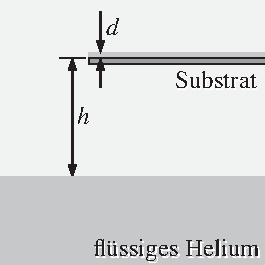
\includegraphics[width=3.5cm]{theo_helium_filme/saturated_films}} \quad
        \plotlink{filmdicke}{\includegraphics[width=\ssmallwidth]{theo_helium_filme/filmdicke}}
    \end{center}
    \caption[Filmdicke des Heliumfilms über der Bulk"=Flüssigkeit]{Abhängigkeit der Dicke des Heliumfilms von dem vertikalen Abstand zur Oberfläche des Bulk"=Heliums nach Gleichung~\eqref{eqn:filmdicke} für $\DC=\unit[26]{K}$. Nicht berücksichtigt ist hier die Retardierung des van"=der"=Waals"=Potentials für $d\gtrsim\unit[100]{nm}$.}
\end{figure}

Durch eine Variation der Filmdicke $d$, gesteuert durch den vertikalen Abstand $h$ der Bulk"=Helium"=Oberfläche vom Substrat, kann man somit die Dicke des Heliumfilms auf dem Substrat im experimentell zugänglichen Bereich von ca.\ \unit[25]{nm} bis zu mehr als \unit[90]{nm} variieren. Wie später noch gezeigt wird, verschwindet allerdings die Abhängigkeit der Filmdicke von der Höhe über der Oberfläche der Bulk-Flüssigkeit, wenn man zu größeren Elektronendichten übergeht. Dann üben die Elektronen einen so hohen Druck auf die Oberfläche des Heliumfilms aus, dass die Abhängigkeit vom vertikalen Abstand zum Bulk"=Helium keine Rolle mehr spielt.

\subsubsection{Änderung der Filmdicke bei Beladung mit Elektronen}

Der elektrostatische Druck, den die Elektronen auf die Oberfläche des Heliumfilms ausüben, wächst mit der Elektronendichte und der angelegten Haltespannung. Diese Kraft wird für Elektronendichten höher als \unit[10$^{13}$]{\Em} wichtig und führt dann zur Verringerung der Filmdicke des gesättigten Heliumfilms unter dem 2DES. Dieser Effekt wurde von \name{Etz} \ea~\cite{Etz84} mit Hilfe von Ellipsometrie an Heliumfilmen auf Substraten aus Glas und Silizium untersucht. Die Ergebnisse konnten mit folgender Abhängigkeit der Filmdicke von der gesättigten Elektronendichte $n_s$ und der Dicke des unbeladenen Heliumfilms $d_0$ gut beschrieben werden:
    \begin{equation}
        \label{eqn:beladene_filmdicke}
        d = d_0\left(1+\frac{n_s^2 e^2}{2\varepsilon_0\rho g h}\right)^{-\frac13}\quad.
    \end{equation}
%Siehe hierzu auch V. V. Tatarskii, N. I. Shikina and V. B. Shikin, Sov. Phys. JETP {\bfseries 55}, 444 (1982) und Sov. J Low Temp Phys. {\bfseries 10} No. 2 (1984). \TODO

\begin{figure}[h!tbp]
    \begin{center}
        \begin{minipage}[b]{\smallwidth}
        \plotlink{filmpressure}{\includegraphics[width=\smallwidth]{theo_helium_filme/filmpressure}}
        \end{minipage}
        \hfill
        \begin{minipage}[b]{\textwidth-\smallwidth-\tabcolsep}
            \caption[Beeinflussung der Filmdicke durch die Elektronendichte.]{Abhängigkeit der Dicke des Heliumfilms von der Elektronendichte in Sättigung nach Gleichung~\eqref{eqn:beladene_filmdicke} \cite{Etz84}. Die Anfangsfilmdicken $d_0$ sind $\unit[37]{nm}\;(h=\unit[5]{mm})$, $\unit[29.3]{nm}\;(h=\unit[10]{mm})$ und $\unit[23.3]{nm}\;(h=\unit[20]{mm})$.}\label{fig:filmdicke_elektronendichte}
        \end{minipage}
    \end{center}
\end{figure}

In Abbildung~\ref{fig:filmdicke_elektronendichte} ist gezeigt, wie sich die Dicke eines mit Elektronen beladenen Heliumfilms mit zunehmender Elektronendichte verringert. Hierbei wird deutlich, dass die Abhängigkeit der Filmdicke von ihrem Anfangswert ohne Elektronen bei hohen Elektronendichten immer geringer wird und bei Dichten größer als \unit[$4\times10^{14}$]{\Em} dann völlig verschwindet.
%TODO komischer Satz

\subsubsection{Abhängigkeit der Sättigungsdichte der Elektronen von der Filmdicke}
\label{sssec:theo_film_saettigung}

Nach den nun folgenden Überlegungen zur statischen Bestimmung der Elektronendichte folgt eine zur Bestimmung der wahren Elektronendichte wichtige selbstkonsistente Rechnung, die auch die Effekte der Reduzierung der Filmdicke durch den vorhandenen Elektronendruck berücksichtigt. Eine solche Methode wurde bereits in \cite{guenzler,Mis97} vorgeschlagen und verwendet, allerdings ohne dass die Vorgehensweise zur Berechnung der nach der Methode korrigierten Werte und auch die erhaltenen Ergebnisse diskutiert wurden.

In Analogie zum vorliegenden Experiment wird ein leitfähiges Substrat betrachtet, das mit einer isolierenden Deckschicht bedeckt ist. Ein schematischer Querschnitt durch die Substratoberfläche mit den in den Rechnungen verwendeten Bezeichnungen findet sich in Abbildung~\ref{fig:substrat_schema}. 
\begin{figure}[h!tbp]
	\begin{minipage}[b]{10cm}
		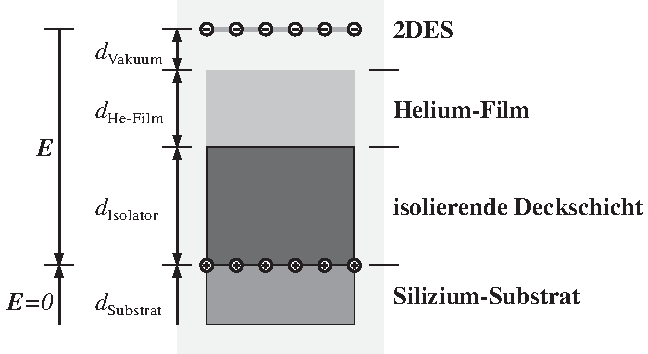
\includegraphics[width=10cm]{theo_helium_filme/electron_density}
	\end{minipage}\hfill
	\begin{minipage}[b]{\textwidth-10cm-\tabcolsep}
		\caption[Schema des Substrataufbaus zur Berechnung der Elektronendichte.]{Schematischer Schnitt durch die Substratoberfläche mit den in den Rechnungen verwendeten Größen. Gezeigt sind nur freie Ladungen und nicht die an den Grenzflächen der Dielektrika lokalisierten Verschiebungsladungen. $d_\text{Vakuum}$ ist der Gleichgewichtsabstand der Elektronen über der Heliumoberfläche von ca.\ \unit[100]{\AA}.}
	\label{fig:substrat_schema}
	\end{minipage}
\end{figure}

Die Elektronendichte in Sättigung wird definitionsgemäß erreicht, wenn der Raum oberhalb des 2DES feldfrei wird. Somit werden keine weiteren Elektronen durch das elektrische Feld angezogen und die Elektronendichte des 2DES bleibt konstant, obwohl das Filament weiter gepulst wird. Für diesen Fall kann man als Modell des Systems einen horizontal liegenden Plattenkondensator verwenden, dessen obere Platte das 2DES und die untere das leitfähige Silizium"=Substrat repräsentiert. Mit den folgenden bekannten Formeln für einen Plattenkondensator soll nun die Elektronendichte eines 2DES in Sättigung und in Abhängigkeit von der Haltespannung berechnet werden. Der Kondensator mit der Kapazität $C$ besitzt die Ladung $Q$ auf seinen Platten. Die Potentialdifferenz zwischen den Kondensatorplatten der Fläche $A$ ist $U$; $d$ ist der Abstand der Platten. Es gilt: 
\begin{equation}
    \label{eqn:plattenkondensator}
    Q=C\,U\textt{,}
    C=\varepsilon\frac{A}{d}\quad.
\end{equation}
Die Flächenladungsdichte $\nicefrac{Q}{A}$ des 2DES stimmt für den Fall der Beladung in Sättigung mit der Flächenladungsdichte der Elektronen am oberen Rand der leitfähigen Substratschicht überein. Da das 2DES aus dem Reservoir der angebotenen Elektronen schöpft, ohne dass ein zusätzliches Potential ein Rolle spielt, kann man annehmen, dass sich das 2DES wie eine mit der Masse verbundene Kondensatorplatte verhält und somit $U$ an der Kondensatorplatte der Haltespannung $U_\text{clamp}$ gleichsetzen. Die Elektronendichte in Sättigung des 2DES ergibt sich dann nach den Gleichungen~\eqref{eqn:plattenkondensator} zu
\begin{equation}
    \label{eqn:elektronendichte}
    n_s=\frac{Q}{e A}=
    \frac{U_\text{clamp}\varepsilon_0}{e}\frac1{
        \frac{d_\text{Vakuum}}{1}+
        \frac{d_\text{He-Film}}{\varepsilon_\text{r,He-Film}}+
        \frac{d_\text{Isolator}}{\varepsilon_\text{r, Isolator}}}\quad.
\end{equation}
Wie man sieht, ist in dieser einfachen Beziehung die Sättigungselektronendichte des 2DES $n_s$ proportional zur angelegten Haltespannung $U_\text{clamp}$. Aus der weiter unten folgenden selbstkonsistenten Korrektur für dünne Heliumfilme und hohe Elektronendichten ergeben sich dann Abweichungen von diesem linearen Verhalten.

Der mittlere Abstand der Elektronen zur Heliumoberfläche $d_\text{Vakuum}=\left<z\right>$ wird hier berücksichtigt, da sein Beitrag die Größe der Elektronendichte vor allem bei sehr dünnen Heliumfilmen beeinflusst. Die Abhängigkeit dieses Parameters von der Sättigungsfilmdicke wird hier nach der einfachen Näherung von \name{Hu} \ea\ \cite{Hu90} durch
\begin{equation}
	d_\text{Vakuum}\approx\left<z\right>\approx\unit[2]{nm} + 10^{-1}d
\end{equation}
bestimmt, die allerdings nur für Elektronen auf dünnen Heliumfilmen gültig ist.

\subsubsection{Selbstkonsistente Lösung zur Bestimmung der Elektronendichte}

Im Gegensatz zur Situation von sehr geringen Elektronendichten auf Bulk"=Helium ist die Bestimmung des Sättigungswertes der Elektronendichte auf dünnen Heliumfilmen durch die wechselseitige Abhängigkeit der Parameter Filmdicke $d$ und Elektronendichte $n_s$ erschwert. Gerade bei den hier auf Grund der van"=der"=Waals"=Stabilisierung des Heliumfilms erreichbaren höheren Elektronendichten werden die Abweichungen von einer einfachen Abschätzung nach Gleichung~\eqref{eqn:elektronendichte} ohne Berücksichtigung ihrer Filmdickenabhängigkeit signifikant.

Man kann nun versuchen, die reale Elektronendichte mit Hilfe einer selbstkonsistenten Rechnung aus den bereits bekannten Beziehungen~\eqref{eqn:elektronendichte} und \eqref{eqn:beladene_filmdicke} herzuleiten. Die Parameter, die die Elektronendichte und die Filmdicke dann bestimmen, sind
\begin{enumerate}
    \item die am Substrat angelegte Haltespannung $U_\text{clamp}$,
    \item der Höhenunterschied $h$ zwischen Substrat- und Bulk"=Helium"=Oberfläche und
    \item der Aufbau und die dielektrischen Eigenschaften der Substratoberfläche, $d_\text{Isolator},$ $\varepsilon_{r,\text{Isolator}}$, die dielektrischen Eigenschaften des Heliumfilms $\varepsilon_{r,\text{He-Film}}$ und die van-der-Waals Konstante von Helium auf dem Substrat $\DC$. 
\end{enumerate}

Als Startwert für die Filmdicke soll die Dicke des unbeladenen Heliumfilms dienen, wie sie sich aus Gleichung \eqref{eqn:filmdicke} ergibt. Für diese Filmdicke erhält man mit der gegebenen Haltespannung $U_\text{clamp}$ aus Gleichung~\eqref{eqn:elektronendichte} eine Elektronendichte $n_s(i=1)$ für die erste Iteration $(i=1)$. Wenn man nun nach Gleichung~\eqref{eqn:beladene_filmdicke} für die berechnete Anfangsfilmdicke und Elektronendichte $n_s(i=1)$ eine neue Filmdicke unter Elektronenbeladung $d(i=1)$ berechnet, kann man durch wiederholtes Einsetzen der erhaltenen Parameter in die Gleichungen~\eqref{eqn:elektronendichte} und \eqref{eqn:beladene_filmdicke} im Limes selbstkonsistente Werte für $d$ und $n_s$ erhalten:
\begin{equation}
    \begin{aligned}
        d(0) &= d_0\\[2ex]
        n_s(i+1) &= n_s\left(U,d(i), \ldots\right)\ttext{nach \eqref{eqn:elektronendichte}}\\
        d(i+1) &= d\left(d_0,n_s(i+1), \ldots\right)\ttext{nach \eqref{eqn:beladene_filmdicke}} \quad.
    \end{aligned}
\end{equation}
\begin{figure}[h!tbp]
    \centerline{\hfill%
        \subfigure[Konvergenz von $d$]{\plotlink{drec}{\includegraphics[width=\ssmallwidth]{theo_helium_filme/drec}}}\hfill%
        \subfigure[Konvergenz von $n_s$]{\plotlink{nrec}{\includegraphics[width=\ssmallwidth]{theo_helium_filme/nrec}}}\hfill%
    }
    \caption[Konvergenz der selbstkonsistenten Lösung]{Konvergenz der selbstkonsistenten Lösung der Sättigungsfilmdicke und der Sättigungselektronendichte für jeweils zwei Haltespannungen. Gezeigt ist die relative Änderung des berechneten Wertes für den jeweiligen Iterationsschritt.
(Parameter: $h=\unit[1]{cm}$, $d_\text{Substrat}=\unit[200]{nm}$, $d_\text{Vakuum}=\unit[10]{nm}$).}\label{fig:film_rekursion}
\end{figure}
Wie man in Abbildung~\ref{fig:film_rekursion} sehen kann, konvergieren die hierbei erhaltenen Parameter sehr schnell. Nach einigen Iterationen der hier vorgestellten Methode ändern sich die Werte von $d$ und $n_s$ nur noch geringfügig und man erhält eine gute Näherung für die wahre Filmdicke und Elektronendichte.

%TODO Rechtschreibung Weiteren groß/klein?
Im Weiteren wird immer eine zehnfache Iteration der hier vorgestellten Methode zur selbstkonsistenten Berechnung der Werte der Elektronendichte und Filmdicke Verwendung finden.

\subsubsection{Analyse der selbstkonsistenten Lösung}

\begin{figure}[h!tbp]
	\begin{center}
		\subfigure[Variation der Filmdicke]{\plotlink{uclamp_d_dep2}{\includegraphics[width=\smallwidth]{theo_helium_filme/uclamp_d_dep2}}}%
		\subfigure[Variation der Elektronendichte]{\plotlink{uclamp_n_dep2}{\includegraphics[width=\smallwidth]{theo_helium_filme/uclamp_n_dep2}}}
	\end{center}
	\caption[Elektronendichte auf PMMA, selbstkonsistente Rechnung]{Abhängigkeit {\bfseries (a)} der Elektronendichte $n_s$ und {\bfseries (b)} der Filmdicke $d$ von der angelegten Haltespannung $U_\text{clamp}$ nach selbstkonsistenter Rechnung. Parameter für PMMA: $h=$\unit[1]{cm}, $d_\text{Substrat}=$\unit[200]{nm}, $\varepsilon_\text{Substrat}=1.7$.}\label{fig:film_selbstkonsistent2}
\end{figure}

Der Verlauf von $d$ und $n_s$ in Abbildung~\ref{fig:film_selbstkonsistent2} für ein \unit[200]{nm} PMMA/Silizium"=Substrat zeigt den deutlichen Einfluss des Elektronendrucks auf die Filmdicke. Im Gegensatz dazu fällt die Korrektur zur Elektronendichte weitaus geringer aus und ist im Anbetracht der sonstigen Fehler bei der Bestimmung der Parameter, die der Elektronendichte zu Grunde liegen, zu vernachlässigen.

Der Einfluss auf die Elektronendichte wird für Elektronen auf einem \unit[200]{nm} \SiO/Silizium"=Substrat stärker, wie es in Abbildung~\ref{fig:film_selbstkonsistent} zu sehen ist. Der Einfluss der Änderung der Filmdicke durch den Elektronendruck auf \SiO"=Substrat wird schon bei sehr geringen Elektronendichten um $\unit[10^{14}]{\Em}$ merkbar und die Abweichung der Elektronendichte von der linearen Abhängigkeit von $U_\text{clamp}$ nach \eqref{eqn:elektronendichte} ist bei $U_\text{clamp}=\unit[2]{V}$ mehr als \unit[50]{\%}. Wie man sieht, geht die Dicke des Heliumfilms bei der maximalen Elektronendichte schon auf unter \unit[4]{nm}. Vor allem bei 2DES auf Substraten mit leitfähiger Oberfläche wird dieser Effekt der Filmdickenreduktion noch stärker sein. In diesem Bereich sind dann sehr glatte Substrate nötig, um das frühe Einsetzen des Tunnelns von Elektronen an Oberflächenrauigkeiten zu vermeiden. Dieser Effekt limitiert die maximal erreichbare Elektronendichte und soll später noch diskutiert werden. Aber auch bei Substraten, die eine isolierende Deckschicht besitzen, wird so der Einfluss der Oberflächenrauigkeit bei höheren Elektronendichten stärker. 
\begin{figure}[h!tbp]
	\begin{center}
		\subfigure[Variation der Filmdicke]{\plotlink{uclamp_d_dep}{\includegraphics[width=\smallwidth]{theo_helium_filme/uclamp_d_dep}}}%
		\subfigure[Variation der Elektronendichte]{\plotlink{uclamp_n_dep}{\includegraphics[width=\smallwidth]{theo_helium_filme/uclamp_n_dep}}}
	\end{center}
	\caption[Elektronendichte auf \SiO, selbstkonsistente Rechnung]{Abhängigkeit {\bfseries (a)} der Elektronendichte $n_s$ und {\bfseries (b)} der Filmdicke $d$ von der angelegten Haltespannung $U_\text{clamp}$ nach selbstkonsistenter Rechnung. Parameter für \SiO: $h=$\unit[1]{cm}, $d_\text{Substrat}=$\unit[200]{nm}, $\varepsilon_\text{Substrat}=4.5$.}\label{fig:film_selbstkonsistent}
\end{figure}

Unterschiedliche Substratmaterialien und die Art des Dielektrikums der Isolator"=Schicht haben, wenn man von der Güte der Substratoberfläche absieht, im Prinzip keinen Einfluss auf die erreichbaren Elektronendichten. Die Parameter der Isolierschicht $d_\text{Isolator}$ und $\varepsilon_{r,\text{Isolator}}$ ändern nur die lineare Skalierung der Abhängigkeit $n_s(U_\text{clamp})$; Kurvenscharen dieser Abhängigkeit liegen für verschiedene Sätze von Parametern der Isolierschicht übereinander. D.~h.\ der einzige Einfluss der Verwendung von Isolierschichten mit verschiedenem $\varepsilon_{r,\text{Isolator}}$ ist die im Abschnitt~\ref{ssec:phasediag_films} genauer beschriebene Modifikation des Phasendiagramms des 2DES.

\subsection{Stabilität des Heliumfilms bei hohen Elektronendichten}
\label{ssec:film_stability}

Verschiedene Autoren \cite{Ike81,Etz84,Hu90} kommen zu der Schlussfolgerung, dass dünne Heliumfilme auf dielektrischen Substraten bei sehr hohen Elektronendichten stabil bleiben. Nur die Wahrscheinlichkeit für das Tunneln von Elektronen durch die Barriere von \unit[1]{eV} nimmt mit dünner werdendem Film zu und muss vor allem bei Heliumfilmen auf leitfähigen Substraten beachtet werden.

Auf dünnen Heliumfilmen spielen zwei Effekte zur Stabilisierung/Destabilisierung der Filmoberfläche eine Rolle:
\begin{enumerate}
    \item der Deformationen der Oberfläche ausgleichende van"=der"=Waals"=Druck $\propto\frac1{d^4}$ und
    \item die Verstärkung der Bildladung bei zunehmender Dielektrizitätskonstante des Substrats.
\end{enumerate}
Ein Indikator für die Stabilität einer Heliumoberfläche gegenüber der Beladung mit Elektronen ist die Dispersionsrelation der Ripplonen.
Diese erhält, wie in \name{Ikezi} \ea{} \cite{Ike81} gezeigt, im Vergleich zur Situation auf Bulk"=Helium~\eqref{eqn:ripplon_dispersion_bulk} einen zusätzlich zur Erdbeschleunigung auftretenden, stabilisierenden van-der-Waals-Term $\frac{3\alpha}{\rho_\text{He} d^4}$. Für dünne Filme gilt:
    \begin{equation}
        \label{eqn:ripplon_dispersion:film}
        \omega^2_\text{ripplon}=\frac{\rho_s}{\rho_\text{He}}
			\left[\left(\frac{3\alpha}{\rho_\text{He} d^4}+g\right)k_\text{ripplon}+
            \frac{\sigma_\text{lv}}{\rho_He} k^3_\text{ripplon}-
			\frac{4\pi n^2e^2}{\rho_\text{He}} k^2_\text{ripplon}
				F(k_\text{ripplon},\varepsilon)\right]\tanh(k d)\quad.
    \end{equation}
Es wird angenommen, dass der Heliumfilm bis zur Sättigung mit Elektronen beladen ist und somit das elektrische Feld oberhalb der Elektronenschicht verschwindet. Die Funktion $F$ berücksichtigt die Auswirkung der Bildladung im Substrat. Für dielektrisches Material ist $F\approx\varepsilon$ und für Metalle gilt $F(d)=\coth(k_\text{ripplon}d)$.

Nach Analyse der Dispersionsrelation~\eqref{eqn:ripplon_dispersion:film} erhalten \name{Ikezi} \ea{} für \unit[10]{nm} Filmdicke eine untere Grenze  von \unit[$10^{15}$]{\Em} für die Instabilität. Des Weiteren weisen sie auf das Problem des Tunnelns von Elektronen bei diesen dünnen Filmen und hohen Haltefeldern hin.

Experimente zur Stabilität von Heliumfilmen auf verschiedenen Substraten wurden von \name{Etz} \ea{} \cite{Etz84} durchgeführt. Hierbei wurden Elektronendichten höher als \unit[$10^{15}$]{\Em} erfolgreich erzeugt. Allerdings zeigte sich bei den Messungen mit leitfähigem Silizium"=Substrat, dass die durch den Elektronendruck verursachte Reduzierung der Filmdicke nach Beenden der Beladung sofort wieder in Richtung des Startwertes relaxiert. Dies wird als Hinweis auf das Tunneln von Elektronen an Spitzen der Substratrauigkeit gesehen.

\subsubsection{Stabilitätskriterien}
Eine weitergehende Analyse der Stabilität von hohen Elektronendichten auf dünnen Heliumfilmen über verschiedenen Substraten wurde von \name{Hu} und \name{Dahm} durchgeführt (\cite{Hu90} und \cite{Dah91}).

Bei metallischen Substraten ist die gesättigte Elektronendichte immer nahe an der Stabilitätsgrenze. Das Bildladungspotential ist invers von der Filmdicke abhängig, aber die zusätzliche Entfernung des Elektrons vom Substrat aufgrund der Nullpunktsschwingung der Elektronen reduziert das effektive Haltefeld soweit, dass der Heliumfilm stabil bleibt.

Eine Schlussfolgerung von \cite{Hu90} ist, dass in Sättigung mit Elektronen beladene Heliumfilme für alle Elektronendichten gegenüber Oberflächenfluktuationen stabil sind. Für Substrate mit leitfähiger Oberfläche steigt allerdings mit abnehmender Filmdicke die Tunnelwahrscheinlichkeit und verhindert eine weitere Erhöhung der Elektronendichte ab Heliumfilmdicken unter \unit[3.5]{nm}. Für metallische Substrate geben \name{Hu} und \name{Dahm} deshalb eine maximal erreichbare Elektronendichte von ungefähr $\unit[1.5\times10^{15}]{\Em}$ an. Zusätzlich merken sie an, dass die Oberflächenrauigkeit auf realen Substraten schon bei weit geringeren Elektronendichten zum Einsetzen von Tunnelprozessen führen wird und dies das Erreichen von hohen Elektronendichten unmöglich macht. Sie schlagen auch vor, durch Aufbringen eines dünnen Films von festem Wasserstoff mit der Dicke von einigen Monolagen das Tunneln von Elektronen in das Substrat zu verringern. Dadurch könnte man die maximal erreichbare Elektronendichte um etwa eine Größenordnung erhöhen -- dann wird allerdings wieder das Tunneln von Elektronen direkt in das Substrat relevant.

\chapter{Stand der Forschung}
Für die Untersuchung des Phasendiagramms eines 2DES auf dünnen Heliumfilmen ist die  verlässliche Erzeugung von hohen Elektronendichten eine unbedingte Voraussetzung. Nachdem das System Elektronen auf Bulk"=Helium nach seiner Entdeckung sehr umfassend  erforscht wurde, gab es erst über zehn Jahre später fundierte Erkenntnisse über den Grenzbereich eines 2DES auf dünnen Heliumfilmen. Eine Ursache für diese lange Zeitspanne ist sicherlich die große Herausforderung der reproduzierbaren Präparation des 2DES auf dünnen Heliumfilmen. Im Gegensatz zu Bulk"=Helium spielt hier der Einfluss des darunter liegenden Substrats eine große Rolle und erschwert es, von Messung zu Messung vergleichbare Ausgangsbedingungen sicherzustellen. 
  
\section{Elektronensysteme hoher Dichten}
\name{Etz} \ea\ \cite{Etz84} erreichten auf einem unbehandelten Silizium"=Substrat, also einer nur mit der natürlich vorhandenen Oxidschicht bedeckten Oberfläche, im Nichtgleichgewicht Elektronendichten bis zu \unit[$7\times10^{14}$]{\Em}. Allerdings konnte diese hohe Elektronendichte nur bei kontinuierlicher Nachlieferung von Elektronen gehalten werden und relaxierte nach Abschalten der Elektronenquelle innerhalb von Minuten auf deutlich geringere Werte unter \unit[$5\times10^{13}$]{\Em} zurück. Im Laufe dieser Experimente wurde die Abhängigkeit der Dicke des Heliumfilms von der Elektronendichte im 2DES \eqref{eqn:beladene_filmdicke} mit Hilfe der optischen Methode der Ellipsometrie am Heliumfilm bestimmt. Damit wurde eine Möglichkeit zur Verfügung gestellt, die Elektronendichte auf dünnen Heliumfilmen unabhängig von der an das Substrat angelegten Haltespannung zu bestimmen und somit den daraus bestimmten Dichtewert zu verifizieren.

Eine erste Messung des Phasenübergangs von der Elektronenflüssigkeit in das Wigner"=Regime auf einem gesättigten Heliumfilm wurde von \name{Jiang} \ea\ \cite{Jia88} gezeigt. Hierbei wurde auf einem Glassubstrat eine maximale Elektronendichte von \unit[$1.3\times10^{14}$]{\Em} erreicht. Die von den theoretischen Arbeiten von \name{Peeters} \ea{} \cite{Pee83, Pee84} vorhergesagte Modifikation des Phasendiagramms von 2DES auf dünnen Heliumfilmen konnte qualitativ verifiziert werden. Eine Korrektur des theoretischen Modells an die gemessenen Daten wurde von \name{Saitoh} \cite{Sai89} für eine quantitative Interpretation der Daten von \name{Jiang} \ea\ gegeben.

Um die Probleme der Detektion des Beweglichkeitssignals eines 2DES auf dünnen Heliumfilmen zu verringern, wurde versucht, die Messfrequenz, die bei den bekannten Messungen mit Sommer"=Tanner"= oder Corbino"=Geometrie in der Größenordnung von \unit[100]{kHz} liegt, weiter zu erhöhen. Eine Erhöhung der Messfrequenz bei vergleichbarer Amplitude des elektrischen Feldes hat eine Reduzierung der Schwingungsamplitude der Elektronen zur Folge. Bei geringerer Schwingungsamplitude erhoffte man sich eine schwächere Abhängigkeit der gemessenen Signale von den Einflüssen der vorhandenen Substratrauigkeit -- dies war der Beginn einer Reihe von Mikrowellenmessungen.

\section{Bisherige Mikrowellenmessmethoden}
\subsection{Messung der Transmission bei konstanter Anregungsfrequenz}
Von \name{Lehndorff} \cite{lehndorff} wurden die ersten Messungen an einem 2DES auf dünnen Heliumfilmen im Inneren eines Mikrowellen"=\HR s durchgeführt. Von Beginn an wurde wegen seiner geringen Leitfähigkeit bei tiefen Temperaturen Silizium als Substratmaterial verwendet. Für das Isolatormaterial zwischen dem Silizium und dem das 2DES tragenden Heliumfilm wurden isolierende Folienmaterialien, wie z.\ B. Hostaphan eingesetzt.

Zu Beginn der Mikrowellenmessungen war die naheliegende Messmethode, die Mikrowellen mit konstanter Frequenz in das System einzustrahlen, um somit z.~B. mit Hilfe einer an der Flanke der Mikrowellenresonanz liegenden Messfrequenz die Änderung der Resonanzfrequenz oder der Amplitude der Resonanz zu detektieren. Dies hat allerdings den Nachteil, dass es hierbei nicht möglich ist beide Größen voneinander zu trennen, da hierzu nicht genügend Messparameter zur Verfügung stehen.

\subsection{Regelung der Anregungsfrequenz auf die Position der Resonanzkurve}
Einen Fortschritt in der Messgenauigkeit und in der Trennung von Frequenz- und Amplitudenmessung brachte die Verwendung des in \cite{neser,guenzler} beschriebenen Lock"=In"=Regelkreises, mit dessen Hilfe die Messfrequenz immer mit der Resonanzfrequenz des \HR s mitgeführt wird. Diese Messmethode wird in Abschnitt~\ref{ssec:old_method} genauer beschrieben. 

Der Lock"=In"=Regelkreis hat den Nachteil, dass eine Änderung der Form der Resonanzlinie außerhalb der angenommenen mathematischen Beziehung von Güte und Transmission nicht zweifelsfrei detektiert werden kann, z.~B. bei einer Verkippung der Resonanzfrequenz und Modifikation der Linienbreite infolge von Leitungsreflexionen\footnote{In diesem Fall wird die frequenzabhängige Amplitude der gemessene Transmission durch einer Sinusoszillation mit einer Periode in der Größenordnung von \unit[10]{MHz} moduliert.}. Außerdem ergibt sich, wie in Abbildung~\ref{fig:absorption} im Abschnitt~\ref{sec:transquality} zu sehen ist, bei hoher Absorption des Elektronensystems eine Abweichung von der vorausgesetzten Abhängigkeit der Güte von der gemessenen Transmission. 

Ein Vorteil dieses Aufbaus ist allerdings, dass man schnelle Änderungen der Eigenschaften des Hohlraumresonators detektieren kann. Die Regelschleife wird mit der Messfrequenz des Lock"=In"=Verstärkers von einigen $\unit{kHz}$ betrieben, deshalb kann man hiermit auch noch Änderungen der Mikrowellen"=Resonanzkurve detektieren, die in der Größenordnung von Millisekunden liegen (wie z.B. der Einfluss des Filamentpulses auf die Resonanz oder die Auswirkungen der Bewegung der Oberfläche des flüssigen Heliums im Resonator).

\section{Vergleich einiger bisher durchgeführter Messungen}

\begin{table}[h!tp]
\begin{minipage}{0.98\textwidth}
\small
\begin{center}
\begin{tabular}{|r|c|c|c|c|c|}\hline
				& \cite{neser}& \cite{guenzler}\footnote{mit Korrektur nach \cite{bitnar}} & \cite{Gue96} & \cite{Mis97} & diese Arbeit\\\hline\hline
PMMA							& (PFPE)	& & & & \\\hline
Schichtdicke	 [nm]		& 5000	& & & & 100	\\
DK $\varepsilon_r$	& 1.7	&	&	& 2.2	& 1.7	\\
$T$ [K]				& 1.27	& & & & 1.29 \\
$d_0$ [nm]	& 30	& & & & 32 \\\hline
$n_\text{crit., WC}$ [$10^{14}]{\Em}$]	
										&	$\approx$120&	&	& 0.35	& 0.4 \\
$\Gamma_{WC}$	&	&	&	&	& 117 / 125	\\\hline\hline
\SiO								&	&	&	&	&	\\\hline
Schichtdicke	 [nm]		&	200 & 260	& 500	&	& 200	\\
DK $\varepsilon_r$	&	& 5 & 4 & & 4.5	\\
$T$ [K]				&	1.27 & 1.3 & & & 1.2	\\
$d_0$ [nm]	&	40 & 40 & & & 33		\\\hline
$n_\text{crit., WC}$ [$\unit[10^{14}]{\Em}$]
										&	2 & 4	& 1.3	&	& 2.0		\\
$\Gamma_{WC}$	&	& 160& & & 181/240	\\\hline
$n_\text{crit., QM}$ [$\unit[10^{14}]{\Em}$]
										&	& 33	& 4	& & 24	\\
$\Gamma_{QM}$	&	&	&	&	&	100/125	\\\hline
\end{tabular}
\end{center}
\end{minipage}
\caption{Vergleich verschiedener Resultate für 2DES auf dünnen Heliumfilmen.}
\label{tab:compare}
\end{table}

In Tabelle~\ref{tab:compare} sind charakteristische experimentelle Ergebnisse aus verschiedenen Veröffentlichungen von Messungen an 2DES auf dünnen Heliumfilmen aufgeführt. Deutlich wird hier eine starke Streuung der erhaltenen Gamma"=Werte für den Wigner"=Übergang. Auch bei den Veröffentlichungen \cite{guenzler,Gue96} zum sog.\ Quantenschmelzen, also dem Übergang vom Wigner"=Regime in das entartete Fermigas, finden sich stark abweichende Ergebnisse. Ein immer vorhandener Unsicherheitsfaktor ist die Bestimmung der aktuellen Elektronendichte aus der Haltespannung. Zum einen ist es für die Gültigkeit der erhaltenen Dichtewerte wichtig, dass sich das 2DES in Sättigung befindet (d.~h.\ $\vec E=0$ oberhalb des 2DES) und weiterhin spielen auch durchgebrochene Oberflächenladungen eine Rolle, da sie die scheinbare Sättigungsdichte zu höheren Elektronendichten verschieben.

\begin{figure}[h!tp]
	\begin{center}
	\subfigure[\cite{guenzler} mit Korrektur nach \cite{bitnar}]{%
		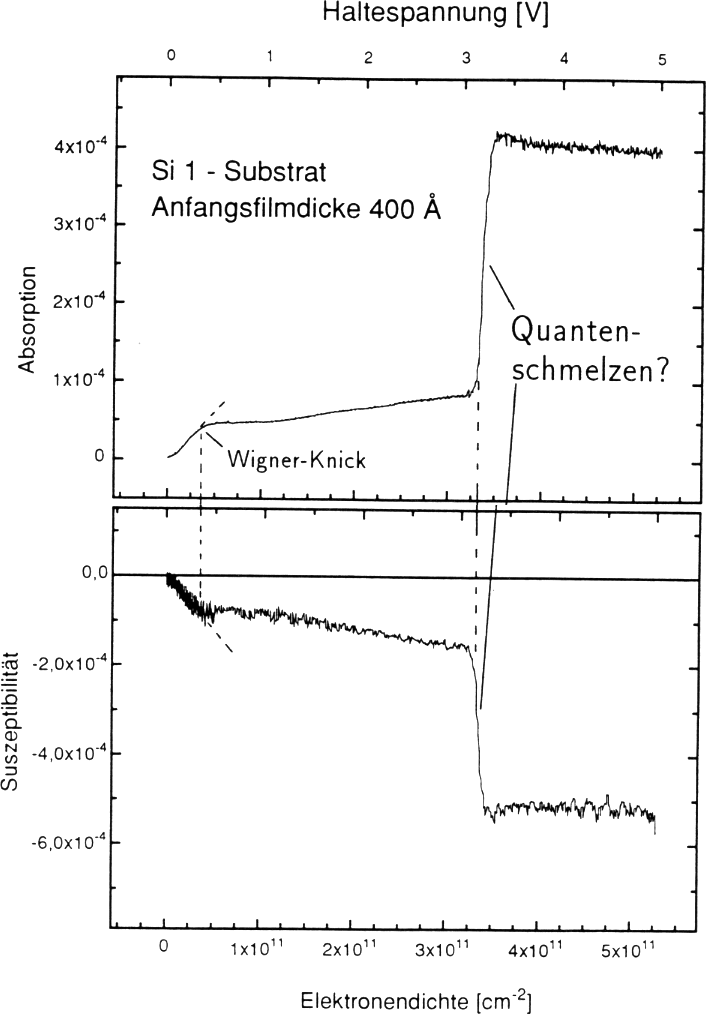
\includegraphics[width=\ssmallwidth]{stand_der_forschung/Bit95}}%
	\hspace{1cm}%
	\subfigure[\cite{Gue96}]{%
		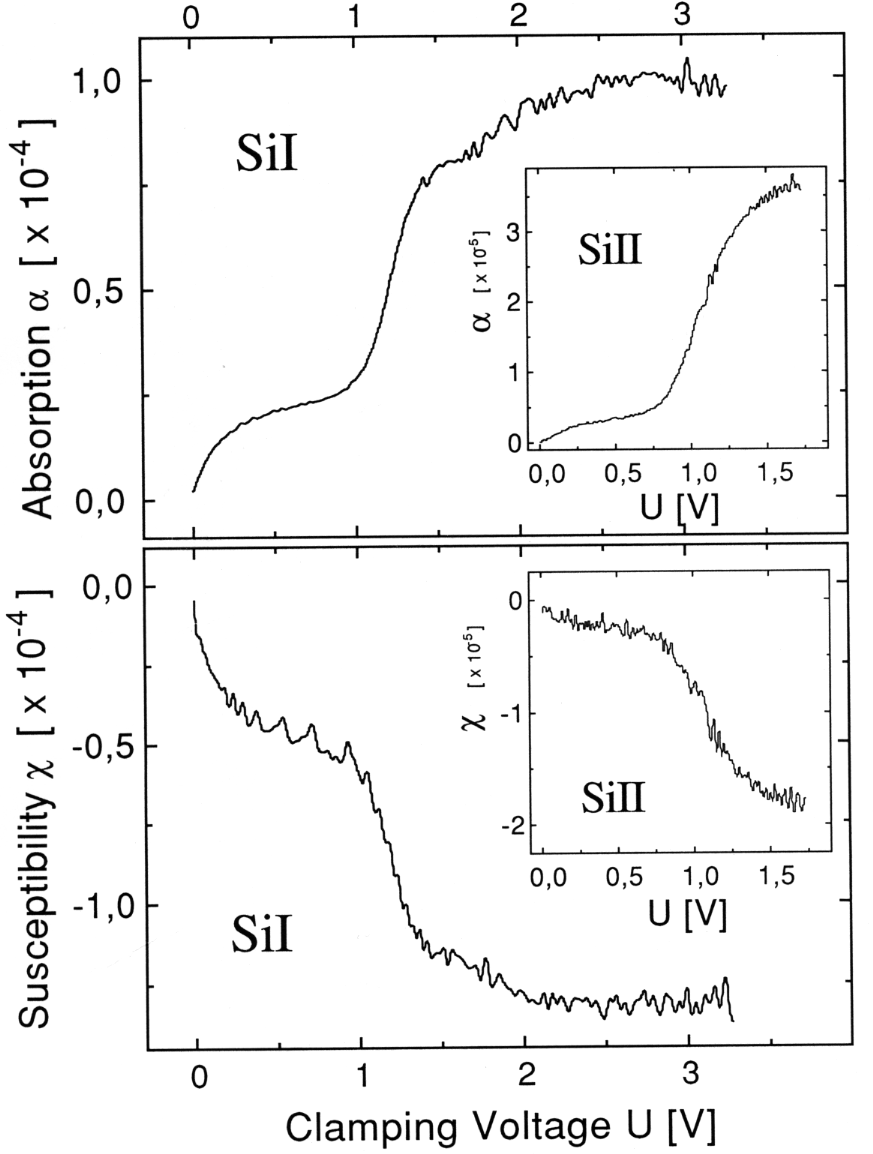
\includegraphics[width=\ssmallwidth]{stand_der_forschung/Gue96}}%
	\end{center}
	\caption{Bisher veröffentlichte Messungen des sog.\ Quantenschmelzens.}
	\label{fig:oldQM}
\end{figure}
In Abbildung~\ref{fig:oldQM} sind beide bisher veröffentlichte Messungen des sog.\ Quantenschmelzens gezeigt. In der Doktorarbeit von \name{T. Günzler} \cite{guenzler} wurden erstmals Anzeichen für einen Phasenübergang vom Wigner"=Festkörper zum entarteten Fermigas entdeckt. Allerdings wurden die hierbei erreichten Elektronendichten offensichtlich wegen der Annahme einer zu geringen Dicke der \SiO"=Deckschicht der Substrate um ca.\ einen Faktor 2.5 überschätzt. Die Filmdicke der Deckschicht wurde in der Diplomarbeit von \name{Bitnar} \cite{bitnar} jedoch nachgemessen und die bisher erhaltenen Elektronendichten korrigiert. Die darauffolgende Veröffentlichung von \name{Günzler} \ea\ \cite{Gue96} zeigt einen weiteren experimentellen Hinweis auf einen derartigen Phasenübergang.
 
Wenn man die experimentellen Ergebnisse zu den Phasenübergängen in das Fermi"=Regime in Tabelle~\ref{tab:compare} und Abbildung~\ref{fig:oldQM} {\bfseries (a)} und {\bfseries (b)} vergleicht, sieht man z.\ B. deutliche Unterschiede im Verhältnis der gemessenen kritischen Dichten $n_\text{crit., QM}$ und $n_\text{crit., WC}$. Dieses liegt bei \cite{guenzler} und dem in dieser Arbeit gezeigten Ergebnis bei ungefähr 10, während es bei \cite{Gue96} nur ca.\ 3 ist. 
 
\enlargethispage{\baselineskip}
Da der in Abbildung~\ref{fig:oldQM} {\bfseries (b)} gezeigte Wigner"=Knick vor allem bei der Probe SiII sehr ausgeschmiert ist, liegt die Vermutung nahe, dass dieser Teil der Messkurve als Artefakt ähnlich dem bei der zweiten Kurve in Abbildung~\ref{fig:pmma_reproduce} {\bfseries (a)} sichtbaren scheinbar früheren Beginn der Beladung interpretiert werden kann. Dieses Verhalten wurde bei der experimentellen Aufnahme von Serien von Beladekurven häufig beobachtet. Nach dem Durchlaufen einiger Beladezyklen scheint die Beladung mit Elektronen schon bei geringeren Haltespannungen einzusetzen. Zusätzlich erhält man beim Übergang in das übliche Drude"=Verhalten einen zweiten Knick im Verlauf der Transmission.

In der Abbildung~\ref{fig:qm_wigner} wurden die aus der Abbildung~\ref{fig:oldQM} {\bfseries (b)} digitalisierten Daten unter der Annahme ausgewertet, dass der in den Absorptionsdaten deutlich sichtbare Phasenübergang nicht ins Quanten"=Regime führt, sondern den bekannten Übergang zum Wigner"=Festkörper darstellt.
\begin{figure}[h!tbp]
	\centerline{
	\subfigure[digitalisierte Daten nach \cite{Gue96}]{\plotlink{Gue96_test}{\includegraphics[width=\smallwidth]{stand_der_forschung/Gue96_test}}}\hfill%
	\subfigure[Auswertung des \name{Wigner}"=Übergangs: {$n_\text{crit}=\unit[1.4\times10^{14}]{\Em}$},  $\Gamma=214$]{\plotlink{Gue96_test2}{\includegraphics[width=\smallwidth]{stand_der_forschung/Gue96_test2}}}}
	\caption[Alternative Interpretation der Daten aus \cite{Gue96}]{Andere Möglichkeit der Interpretation der Messdaten von \cite{Gue96}. Könnte es sich hierbei um einen \name{Wigner}"=Übergang handeln? (siehe Text)}
	\label{fig:qm_wigner}
\end{figure}
\enlargethispage{2\baselineskip}
Die erhaltenen Daten $n_\text{crit}=\unit[1.4\times10^{14}]{\Em}$ und $\Gamma=214$ liegen durchaus im erwarteten Bereich.
Leider waren die Originaldaten der Messung nicht verfügbar, die zur Überprüfung dieser Vermutung einen tieferen Einblick in den gesamten Ablauf und der Vorgeschichte des dargestellten Ausschnitts der Messung ermöglichen würden.
 


\chapter{Experimenteller Aufbau und Messmethoden}
	\label{chap:exp}

\section{Kryostat und Messaufbau}

Für die im Rahmen dieser Arbeit durchgeführten Experimente wurde ein einfacher Helium"=Badkryostat verwendet. Die Messzelle am unteren Ende des Kryostateneinsatzes kann in das Helium"=Dewargefäß eingebracht werden, wie in Abbildung~\ref{fig:kryostat} zu sehen ist.

\begin{figure}[h!tbp]
	\begin{center}\includegraphics{exp_aufbau/nwa_setup}\end{center}
	\caption[Der verwendete Messaufbau]{Der verwendete Messaufbau. Für Messungen mit Variation des Magnetfelds wurde eine senkrechte supraleitende Magnetspule außerhalb der Messzelle angebracht.}
	\label{fig:kryostat}
\end{figure}

Im Weiteren werden die einzelnen Komponenten des experimentellen Aufbaus genauer beschrieben.

\section{Thermometrie}
Zur Bestimmung der Temperatur des \HR s dient eine geeichte Germanium"=Diode, die direkt am Resonator befestigt ist. Zur Temperaturmessung des Helium"=Bades befindet sich am Boden des Dewargefäßes ein Allen"=Bradley Kohlewiderstand. Desweiteren befindet sich dort auch ein Heizwiderstand, mit dessen Hilfe der Temperaturregler die Temperatur des Heliumbads und somit auch die des darin enthaltenen Experiments regeln und stabilisieren kann. Diese Regelung kann die Temperatur der Messzelle im Bereich von $1.2$ bis \unit[1.8]{K} mit einer Genauigkeit, die kleiner als \unit[0.5]{mK} ist einstellen. Eine weitere, von der beschriebenen Methode unabhängige, Temperaturmessung kann über den in der mit flüssigem $^4$He gefüllten Zelle herrschenden Gasdruck bewerkstelligt werden. Die Temperatur lässt sich über die Dampfdruckkurve von $^4$He bestimmen.
 
\section{Erzeugung von Elektronen}
Bei allen im Rahmen dieser Arbeit durchgeführten Experimente an 2DES werden die Elektronen mittels Glühemission von einem Wolframfilament erzeugt. Die dabei verwendeten Filamente sind Miniaturglühbirnen, deren Glaskörper mit einer Zange angebrochen und entfernt wurden. Bei Raumtemperatur kann man sie bei typischerweise \unit[10]{mA} Strom und \unit[1]{V} Spannung betreiben (d.\,h.\ ihr Widerstand im Betrieb ist ca.\ \unit[100]{$\Omega$} und bei Raumtemperatur ca.\ \unit[20]{$\Omega$}). Bei Temperaturen um \unit[4]{K} sinkt der Kaltwiderstand der Filamente auf bis zu $2$ bis $\unit[3]{\Omega}$ ab.

Um den Wärmeeintrag in das Experiment so gering wie möglich zu halten und auch wegen der besseren Dosierung, werden die Filamente gepulst betrieben. Dabei liegt die Pulslänge im Bereich von $10$ bis $\unit[500]{ms}$ und die Pulsamplitude bei ca.\ \unit[1.2]{V}. Damit das Filament seine Arbeitstemperatur erreicht, muss zu Beginn des Pulses ein starker Strom fließen können. Um den Aufwärmvorgang der Filamente am Beginn des Pulses zu beschleunigen, wurden diese nach \cite{kimitoshi} mit einer niederohmigen\footnote{
Der Leitungswiderstand bei im Experiment üblichen Temperaturen beträgt hier nur einige Ohm.} Zuleitung aus Kupfer angeschlossen. Wenn man eine Konstantspannungsquelle, die zu Beginn des Pulses bis zu \unit[100]{mA} liefern kann, zum Treiben des Filaments verwendet, hat das zur Folge, dass das Filament bereits nach sehr kurzer Zeit seine Betriebstemperatur erreicht (typischerweise $<\unit[10]{ms}$, siehe auch Abb.~\ref{fig:filament_puls}). Zusätzlich gibt es den Vorteil, dass sich das Filament im Betrieb selbst stabilisiert. Da der Widerstand der Zuleitung im Vergleich zum Arbeitswiderstand sehr klein ist, regelt sich an einer konstanten Spannung der Strom durch das Filament so, dass ein Durchbrennen desselben verhindert wird. Wenn das Filament z.\ B. heißer wird, da der Strom durch die Glühwendel zunimmt, steigt sein Widerstand, was wiederum zur Abnahme des fließenden Stromes führt. Der Nachteil des geringfügig höheren Wärmeeintrages durch die Kupferleitung ist im Vergleich zu den dadurch erhaltenen besseren elektrischen Eigenschaften für die Benutzung im Badkryostaten unerheblich.

\subsection{Typische Filamentkennlinien}
\label{ssec:filament}
\begin{figure}[h!tbp]
	\centerline{\hfill\subfigure[Ersatzschaltbild]{\raisebox{0.5cm}{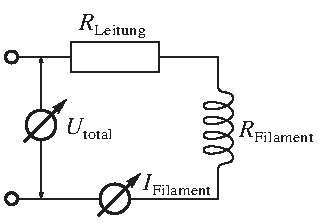
\includegraphics{exp_aufbau/Filamente}}}
	\hfill\subfigure[Verlauf von Strom und Spannung]{\plotlink{filui}{\includegraphics[width=\smallwidth]{exp_aufbau/filui}}}\hfill}
	\caption[Verlauf von Strom und Spannung am Filament]{Schema der Filamentdiagnose und die dabei erhaltenen Daten. In {\bfseries (a)} sieht man das Ersatzschaltbild für den Filamentbetrieb. In {\bfseries (b)} sieht man typische Verläufe von Strom und Spannung während eines Filamentpulses im Experiment.\par(\datalink{2002/mw0201d4/mw0201d4.html}{Messung 01/2002 \#4} Filamentmessung \#100, $U_\text{max}=\unit[1.32]{V}\; I_\text{max}=\unit[104]{mA}$)}
	\label{fig:filamente}
\end{figure}
Zur Kontrolle der Funktion der Filamente wurde der Strom- und Spannungsverlauf während des Pulses aufgezeichnet. Dieser erlaubt so eine genaue Bestimmung der experimentellen Parameter des Filaments.

Aus den in Abb.~\ref{fig:filamente} gezeigten Strom- und Spannungsverläufen eines Filamentpulses kann man über die Bestimmung des Filamentwiderstandes Aussagen über die momentane Temperatur des Filaments machen. Unter der Annahme, dass $R_\text{Leitung}$ während des Pulses konstant und im Bereich einiger Ohm ist, erhält man
\begin{equation}
	\label{eqn:fil_r}
	R_\text{Filament}=\frac{U_\text{total}}{I_\text{Filament}}-R_\text{Leitung}\quad.
\end{equation}

Eine Abschätzung der pro Puls zugeführten Energie kann man aus dem Integral der am Filament aufgewendeten Leistung $P=U\,I$ erhalten, die durch 
\begin{equation}
	\label{eqn:fil_p}
	P_\text{Filament}=U_\text{Filament}I_\text{Filament}=
		\left(U_\text{total}-I_\text{Filament}R_\text{Leitung}\right)I_\text{Filament}
\end{equation}
gegeben ist.
Der vom Strom abhängige Spannungsabfall $U_\text{Leitung}=I_\text{Filament}R_\text{Leitung}$ wird hier zwar noch aufgeführt, später bei der Auswertung der Daten wegen des geringen Leitungswiderstandes jedoch vernachlässigt.

In Abbildung~\ref{fig:filament_puls} sieht man eine Auswertung von Filamentwiderstand und Filamentleistung nach den Gleichungen~\eqref{eqn:fil_r} und \eqref{eqn:fil_p}. Der Filamentwiderstand ist ein Maß für die Temperatur des Filaments und das Integral $E_\text{Fil.}$ über die Filamentleistung ist der Energieeintrag pro Puls in das System, der zum großen Teil verwendet wird, das Filament auf die Arbeitstemperatur aufzuheizen. Die Werte von $R_\text{Fil.}$, $P_\text{Fil.}$ und $E_\text{Fil.}$ sind abhängig vom Gasdruck in der Zelle und auch davon, ob sich das Filament in flüssigem Helium befindet. Alle diese Parameter sind demnach von der Art der Kühlung des Filaments abhängig.

\begin{figure}[h!tbp]
	\centerline{%
	\subfigure[Verlauf des Filamentwiderstands]{\plotlink{filr}{\includegraphics[width=\smallwidth]{exp_aufbau/filr}}}%
	\subfigure[Verlauf der Filamentleistung]{\plotlink{filp}{\includegraphics[width=\smallwidth]{exp_aufbau/filp}}}}
	\caption[Verlauf von Widerstand und deponierter Leistung am Filament]{Der Verlauf {\bfseries (a)} des Filamentwiderstandes und {\bfseries (b)} der im Filament deponierten elektrischen Leistung für die Messdaten aus Abbildung~\ref{fig:filamente} (Aus diesen Daten bestimmte Parameter: $R_\text{max}=\unit[41]{\Omega}$, $R_\text{avg} = \unit[30.4]{\Omega}$, $P_\text{max}=\unit[115]{mW}$, $E=\unit[572]{\grmu J}$). Das Filament erreicht nach ca.\ \unit[10]{ms} seine Endtemperatur. }
	\label{fig:filament_puls}
\end{figure}

\subsection{Durchschnittliche Elektronenproduktion gepulst betriebener Filamente}
\label{ssec:electron_production}

Bei Messungen auf Bulk"=Helium ist durch das Auftreten der elektrohydrodynamischen Instabilität bei $\unit[2\times10^{13}]{\Em}$ ein geeigneter Eichpunkt für die Elektronenproduktion des Filaments vorhanden.
\begin{figure}[t!]
	\centerline{\subfigure[Beladung durch verschiedene Pulsstärken bei $U_\text{clamp}={\unit[100]{V}}$\label{fig:fil_eichung:array}]{\plotlink{fil_eichplot}{\includegraphics{exp_aufbau/fil_eichung}}}}
	\centerline{%
\subfigure[Bestimmung der Instabilität\label{fig:fil_eichung:instab}]{\plotlink{fil_instability}{\includegraphics[width=\smallwidth]{exp_aufbau/fil_instability}}}%
\subfigure[Elektronenproduktion pro Puls\label{fig:fil_eichung:result}]{\plotlink{fil_eichung2}{\includegraphics[width=\smallwidth]{exp_aufbau/fil_eichung2}}}}
	\caption[Eichung der Elektronenproduktion]{Eichung der Elektronenproduktion des Filaments auf Bulk"=Helium. In {\bfseries (a)} ist die Transmission über der Zeit aufgetragen, wobei jeder Datenpunkt einen weiteren Filamentpuls darstellt. Es wurde eine Oberfläche von Bulk"=Helium bei konstanter Haltespannung von \unit[100]{V} und unterschiedlichen Pulsparametern beladen. Aus der anfangs durch die Beladung in {\bfseries (b)} bestimmten Absorption bei Erreichen der elektrodynamischen Instabilität bei \unit[384]{V} kann man die Beladeraten aus den Linienanpassungen von (a) in linearer Näherung abschätzen. In {\bfseries (c)} sieht man die mit dieser Methode bestimmten erhaltenen Elektronenmengen für die Pulse mit unterschiedlichen Parametern. (Messung \datalink{2002/mw0210d1/mw0210d1.html}{mw0210 \#1})}
	\label{fig:fil_eichung}
\end{figure}

Wie in Abbildung~\ref{fig:fil_eichung} zu sehen ist, wurde für eine bestimmte Höhe des Bulk"=Heliums die Spannung ermittelt, bei der die elektrohydrodynamische Instabilität auftritt. Nachfolgend wurden Beladekurven für verschiedene Pulslängen und Pulsamplituden aufgenommen, bei denen eine Spannung an das Substrat angelegt blieb, die geringfügig unter der Spannung bei Instabilität liegt. Dabei kann man in erster Näherung die Transmission als Hinweis auf die Elektronendichte verwenden und die Elektronenproduktion pro Filamentpuls aus der Steigung der abgebildeten Fitgeraden ermitteln.

\subsection{Energieverteilung der emittierten Elektronen}

Die von der Glühwendel emittierten Elektronen besitzen eine gewisse Energieverteilung, die zum einen von ihrer Entstehung durch thermische Emission herrührt und zum anderen durch den linearen Potentialverlauf entlang der Glühwendel bestimmt wird. Die thermische Energie der Elektronen kann man direkt aus ihrer Erzeugung ableiten, wenn man davon ausgeht, dass die thermische Emission bei einer Temperatur von $1500$ bis $\unit[2000]{K}$ stattfindet. Man erhält für diese Temperatur eine korrespondierende thermische Energie von nur ca.\ $\unit[0.2]{eV}$.

Die Energie der emittierten Elektronen, die aus ihrer Beschleunigung durch das elektrische Feld am Filament resultiert, ist einfach abzuschätzen. Da der Betriebswiderstand des Filaments in der Größenordnung von \unit[100]{$\Omega$} liegt und somit viel höher als der Widerstand der Zuleitung ist, fällt fast die gesamte Spannung des Pulses am Filament ab. Wenn man annimmt, dass die Elektronen über die gesamte Länge der Glühwendel emittiert werden, führt dies zu einer Energieverteilung derselben von 0 bis ca.\ \unit[1.2]{eV}.

Die mittlere Stoßzeit von Elektronen in Helium"=Gas bei im Experiment üblichen Temperaturen ist so gering, dass die vom Filament erzeugten Elektronen sehr bald durch Stöße mit den Atomen aus dem Helium"=Gas thermalisieren und daher die Auswirkung ihrer anfänglichen Energie auf den Beladevorgang kaum merkbar ist. Dass die Elektronen sehr gut durch die Stöße mit den Helium"=Atomen im Gasraum abgebremst werden, zeigt sich vor allem bei Messungen mit konstanter, positiver Haltespannung (siehe z.\ B. die Messung der Beladeraten in Abb.~\ref{fig:fil_eichung}). \enlargethispage{\baselineskip}Man findet hierbei kaum Hinweise auf ein verstärktes Durchbrechen der Elektronen.


\section{Bestimmung des Helium"=Füllstands}

\begin{figure}[h!]
	\plotlink{he_level}{\includegraphics[width=\smallwidth]{exp_aufbau/he_level}}
	\hfill
	\begin{minipage}[b]{\textwidth-\smallwidth-\tabcolsep}
		\caption[Abhängigkeit der Resonanzfrequenz vom Helium"=Füllstand]{Beziehung zwischen Resonanzfrequenz und Helium"=Füllstand des mit Substrat bestückten Resonators. Die zwei Knicke in der Mitte bei einem Füllstand von ca.\ \unit[15]{mm} werden durch das Substrat verursacht und können gut als Referenz für das Anpassen der Verschiebung der Resonanzfrequenz an die Höhenskala der Kapazität verwendet werden. Die vertikale Linie bei ca.\ \unit[16]{mm} ist die aus der EHD-Instabilität bestimmte Position der Substrat\-oberfläche. (Messung \datalink{2002/mw0202d3/mw0202d3.html}{02/2002 \#3}, Abschnitt 40)}
		\label{fig:level}
	\end{minipage}
\end{figure}
Zur Bestimmung des Helium"=Füllstands im Resonator kann man die durch das eingefüllte flüssige Helium verursachte Frequenzverschiebung der Resonanz auswerten. Leider ist die Abhängigkeit der Resonanzfrequenz vom Füllstand, wie in Abbildung~\ref{fig:level} zu sehen, nur im Zentrum des Resonators annähernd linear. Man kann zwar unter Vernachlässigung des sich ändernden Resonatorquerschnitts aus dem Frequenzverlauf bei konstanter Abpumprate auf einen linearen Füllstandsverlauf eichen, allerdings gibt es nur einen guten Eichpunkt, der im Frequenzsignal deutlich auszumachen ist -- das Zentrum des Resonators. Wegen der geringen Intensität des elektrischen Feldes der Resonatormoden in der Nähe der Zylinderwand kann man den Start- und Endpunkt des Füllens des Resonators nur sehr schwer festlegen. Hier ist die Frequenzänderung bei Befüllung mit einem Dielektrikum nur sehr gering.

Aufgrund der beschriebenen Schwierigkeit und des Bedürfnisses, den Helium"=Füllstand auch für kleine Füllstände im Resonator für Messungen an Heliumfilmen bestimmen zu können, wurde zusätzlich ein stehender Zylinderkondensator neben dem Resonator in die Zelle eingebaut. Damit lässt sich mit dem flüssigem Helium als Dielektrikum die lineare Abhängigkeit der Kapazität vom Füllstand im Kondensator nutzen, um den Helium"=Füllstand über den kompletten Bereich bis zu einer Genauigkeit von circa $\unit[0.1]{mm}$ zu bestimmen. Die erreichte Genauigkeit ist für die Bestimmung der Filmdicke über den Abstand des Bulk"=Helium"=Füllstandes vom Substrat völlig ausreichend, kann allerdings durch eine genauere Bestimmung der Kapazität noch erhöht werden.

\subsection{Eichung der vertikalen Kondensatorposition}
\label{ssec:level_calib}

Eine Eichung des Helium"=Füllstandes an die vertikale Position des Substrates lässt sich mit Hilfe der elektrohydrodynamischen Instabilität der Elektronen auf Bulk"=Helium durchführen. Bei einer unbekannten Dicke von Bulk"=Helium über dem Substrat bestimmt man durch vorsichtiges Erhöhen der Haltespannung das Einsetzen der elektrohydrodynamischen Instabilität und kann aus der bekannten kritischen Elektronendichte die Dicke des Bulk"=Heliums errechnen. Aus dieser Filmdicke kann man die Position der Substratoberfläche in der aus der Kapazität des Levelkondensators bestimmten Helium"=Füllhöhe bestimmen. Die vertikale Linie in Abb.~\ref{fig:level} soll die so bestimmte Position der Substratoberfläche anzeigen.

\section{Messmethode am Hohlraumresonator}
Üblicherweise liegt die Frequenz von AC-Transportmessungen an 2DES im Bereich
einiger kHz und wird in einer linearen Sommer-Tanner- \cite{Som71} oder einer konzentrischen Corbino"=Elektrodengeometrie realisiert. Wenn man jedoch höhere
Elektronendichten auf dünnen Heliumfilmen erreichen will, ist es schwierig,
eine Transportmessung an den Elektronen mit einem ausreichenden Signal"=Rausch"=Abstand zu realisieren. Denn obwohl das gemessene Signal im Prinzip proportional zu einer Erhöhung der Elektronendichte ist, wird die Substratrauigkeit, die die Beweglichkeit der Elektronen beeinflusst, immer bedeutender. Bei geringen Messfrequenzen ist die durchschnittliche Schwingungsamplitude der Elektronen so groß, dass die Elektronen an der vorhandenen Substratrauigkeit merkbar gestreut werden, was zu einer Reduktion des gemessenen Elektronensignals führt. Abhilfe schafft hier die Verwendung von höheren Frequenzen, um die Transportmessungen bei hohen Elektronendichten auf dünnen Heliumfilmen durchführen zu können. Die Messung der Absorption des 2DES soll bei den zu erreichenden hohen Elektronendichten wegen der auf dünnen Heliumfilmen geringen Mobilität auch bei hohen Messfrequenzen, d.\,h.\ im Mikrowellen"=Frequenzbereich um \unit[10]{GHz} durchgeführt werden. Diese Frequenz ergibt sich aus der Größenordnung der Messanordnung, die im Bereich von Zentimetern liegt. Die Ankopplung an das 2DES geschieht durch die Verwendung von Resonatormoden, deren $\vec E$-Feld parallel zum 2DES liegt.

In Abbildung~\ref{fig:cavity_quer} sieht man einen schematischen Querschnitt durch den verwendeten Hohlraumresonator.
\begin{figure}[h!tbp]
	\centerline{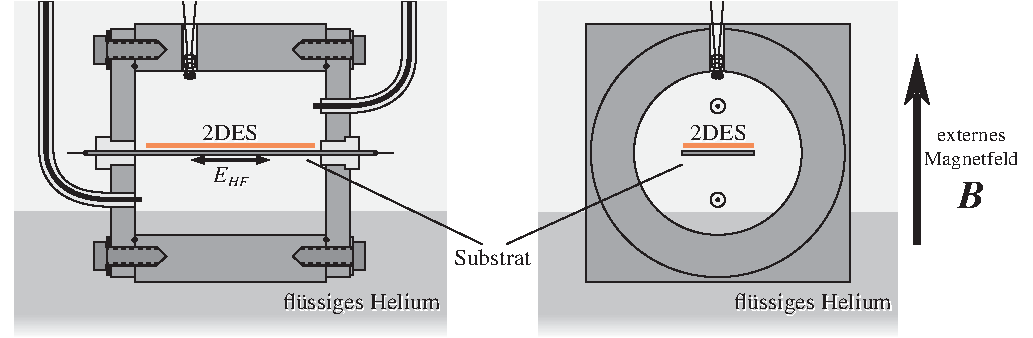
\includegraphics[width=\textwidth]{exp_aufbau/CavityQuerschnitt}}
	\caption[Der Hohlraumresonator im Querschnitt]{Schematische Querschnitte durch den verwendeten Hohlraumresonator. {\bfseries Links} ist ein Querschnitt entlang der Zylinderachse und {\bfseries rechts} ein Querschnitt senkrecht zur Zylinderachse des \HR s zu sehen. Die Länge des Zylinders beträgt \unit[2]{cm} und sein Radius \unit[1.9]{cm}.}
	\label{fig:cavity_quer}
\end{figure}

\subsection{Bisher verwendeter LockIn"=Regelkreis}
\label{ssec:old_method}
\enlargethispage{1\baselineskip}

Der bisher verwendete LockIn-Regelkreis hat den Vorteil, dass das Messsignal sehr schnell Änderungen des Elektronensystems folgen kann. Da die Messfrequenz im Bereich einiger kHz liegt, ist die Antwortzeit der Messung im Bereich von Zehntelsekunden. Dieser Vorteil wird allerdings von dem Nachteil begleitet, dass die Transmission des Resonators nur an einer Frequenz gemessen wird und so die wahre Form der Resonanzlinie verborgen bleibt. Falls die Reflexionen auf den Zuleitungen zum Resonator sehr groß sind oder anderweitig Signalstörungen auftreten, kann man dieses nur schwer diagnostizieren. Das Funktionsprinzip des Regelkreises ist sehr einfach. Der Regelkreis versucht die mittlere Steigung der gemessenen Transmission in einem schmalen Frequenzbereich auf Null zu regeln, d.\,h.\ diese wird genau dann gleich Null, falls die Mittenfrequenz der Frequenzmodulation mit der Resonanzfrequenz des \HR{}s übereinstimmt.

Hierbei wird die Frequenz eines Frequenzgenerators, der im X"=Band\footnote{Dies entspricht einem Frequenzbereich von \unit[8]{GHz} bis \unit[12]{GHz}.} arbeitet, mit Hilfe des Referenzsignals des LockIn-Verstärkers moduliert. Das Signal, das durch den Hohlraumresonator transmittiert, wird über eine Mikrowellendiode mit dem LockIn-Verstärker analysiert und man erhält am Ausgang des LockIn-Verstärkers ein der Steigung der Resonanzkurve am Punkt der Messfrequenz proportionales Regelsignal, dessen Vorzeichen sensitiv auf die jeweilige Flanke der Resonanz des Hohlraumresonators ist. Wenn man das Regelsignal noch in einen PID-Regler einspeist, der daraus einen DC-Offset für das Referenzsignal des LockIn-Verstärkers am Eingang des Frequenzgenerators erzeugt, hat man einen Regelkreis, der sich bei korrekter Justierung immer auf die Frequenz des Maximums der Resonanzlinie einstellt.

Daraus erhält man folgende Parameter der Resonanzfunktion:
\begin{itemize}
	\item Resonanzfrequenz [Hz] und
	\item Amplitude der Transmission an der Resonanzfrequenz [dB].
\end{itemize}
Der Vorteil dieser Methode ist, dass aufgrund der Messfrequenz des LockIn-Verstärkers von einigen Kilohertz das Signal quasi ohne zeitliche Verzögerung messbar ist und somit auch sehr schnelle Änderungen der Resonanz des Hohlraumresonators gemessen werden können, wie sie zum Beispiel nach dem Pulsen des Filaments auftreten. Die Güte der Resonanz wird zu Beginn der Messung abgemessen und im weiteren Verlauf über ihre Proportionalität zur Transmission bestimmt. Im Gegensatz zur in dieser Arbeit verwendeten Messmethode mit dem Netzwerkanalysator wird der \HR\ ständig in Resonanz betrieben, was zur Folge hat, dass der integrale Energieeintrag in das System sehr hoch ist.

\subsection{Neue Messmethode mit Netzwerkanalysator}
\label{ssec:new_method}
Bei Messungen mit Hilfe des Netzwerkanalysators\footnote{Verwendet wurde hier das Modell HP8917D von Hewlett-Packard.} ist die Vorgehensweise eine andere. Mit diesem Gerät ist man in der Lage ein vollständiges Spektrum der Resonanzlinie in der Frequenzumgebung der Resonanz aufzunehmen (typischerweise ist die Frequenzbreite der Abtastung einige MHz,  z.\,B.\ das Doppelte der Linienbreite der Resonanzkurve von ca.\ \unit[10]{MHz}). Für jedes aufzunehmende Spektrum wird die Frequenz der eingestrahlten Mikrowellen kurz über den Messbereich hinweg variiert. Die übliche Zeit für einen Messpunkt, also die Transmission bei einer festen Frequenz ist \unit[0.5]{ms}. Bei typischen 401 Punkten pro aufgenommenem Spektrum ergibt sich eine Gesamtdauer von \unit[200]{ms} pro Spektrum. Nach dieser Messung wird die Mikrowellenemission wieder abgeschalten. Dies ist der größte Unterschied zur bisherigen Messmethode, bei der die Mikrowellen mit genau der Resonanzfrequenz des \HR{}s kontinuierlich in die Zelle eingestrahlt werden, was erhebliche Auswirkungen auf den durchschnittlichen Energieeintrag in das System hat.
	
Die Genauigkeit dieser neuen Messmethode ist allerdings nicht ausreichend, wenn man nur das Resonanzmaximum und dessen Frequenzlage aus den erhaltenen Rohdaten bestimmt. Um eine mit der bisher verwendeten LockIn-Methode vergleichbare Genauigkeit zu erzielen, muss man eine Kurvenanpassung der so erhaltenen Daten der Resonanzlinie an eine einer Lorentzlinie ähnlichen Funktion durchführen:
\begin{equation}
	4A\,\sigma\SQRT{\frac{49x^2 + 4\sigma_\text{res}^2}
	{\left(49\left(x-\nu_\text{res}\right)^2+4\sigma_\text{res}^2\right)
	\,\left(49\left(x+\nu_\text{res}\right)^2+4\sigma_\text{res}^2\right)}}
	+c_0+c_1\nu\quad.
	\label{eqn:resonanzfit}
\end{equation}
\begin{figure}[h!tbp]
	\centerline{%
	\subfigure[Kurvenanpassung der Messdaten]{\plotlink{fitvergleich1}{\includegraphics[width=\smallwidth]{exp_aufbau/fitvergleich1}}}%
	\subfigure[Vergleich der Anpassung mit einem Lorentz-Fit]{\plotlink{fitvergleich2}{\includegraphics[width=\smallwidth]{exp_aufbau/fitvergleich2}}}}%
	\caption[Linienanpassung an die Messdaten der Resonanzkurven]{{\bfseries (a)} Anpassung der Rohdaten nach Gleichung~\eqref{eqn:resonanzfit}. {\bfseries (b)} Vergleich der Linienanpassung nach Gleichung~\eqref{eqn:resonanzfit} mit einem Lorentz"=Fit. (Kurve 1 aus Messung \datalink{2002/mw0205d6/mw0205d6.html}{05/2002 \# 6})}
	\label{fig:fitvergleich}
\end{figure}
Diese Funktion wurde von der Linienanpassung an die Resonanzlinien bei gepulster NMR übernommen \cite{girgl}, die der Autor im Rahmen seiner Diplomarbeit durchgeführt hat. In Abbildung~\ref{fig:fitvergleich} (b) sieht man deutlich das ein Fit mit der einfachen Lorentz-Funktion die Messdaten nicht gut wiedergibt.
Man erhält aus der Kurvenanpassung an Funktion \eqref{eqn:resonanzfit} folgende Parameter:
\begin{itemize}
    \item Resonanzfrequenz $\nu_\text{res}$ [Hz],
    \item Resonanzamplitude $A$ [bel. lineare Einh.],
    \item Linienbreite $\sigma_\text{res}$ [Hz],
    \item konstanter Offset $c_0$ [bel. lineare Einh.] und
    \item linearer Offset $c_1$ [bel. lineare Einh. / Hz].
\end{itemize}
Die beiden Offsetparameter, insbesondere der konstante Offset, sind für die Anpassung realer Messdaten von Nöten. Mit Hilfe des linearen Offsets kann man die Beeinflussung der Messdaten durch nahezu unvermeidbare Leitungsreflexionen erkennen. Diese führen auf Grund der Ausbildung von stehenden Wellen in den Zuleitungen zu einem zusätzlichen von der Frequenz sinusförmig abhängigen Untergrund, dessen Periode groß im Vergleich zur Linienbreite der Resonanzlinie ist und der somit über den Bereich der Resonanz linear genähert werden kann. 

Nach der Linienanpassung wird die daraus bestimmte aktuelle Resonanzfrequenz als Mittenfrequenz des darauffolgenden Frequenzdurchlaufs gesetzt. Somit ist gewährleistet, dass die neue Messmethode mit Hilfe des Netzwerkanalysators immer der Resonanz des Hohlraumresonators folgt -- wie bei der Verwendung des LockIn-Regelkreises.

\begin{figure}[h!tbp]
	\centerline{%
		\subfigure[bisherige Messmethode (LockIn"=Regelkreis)]{\plotlink{vergleich1}{\includegraphics[width=\smallwidth]{exp_aufbau/vergleich1}}}\hfill%
		\subfigure[neue Messmethode (Netzwerkanalysator)]{\plotlink{vergleich2}{\includegraphics[width=\smallwidth]{exp_aufbau/vergleich2}}}}
	\caption[Vergleich der bisherigen und neuen Messmethoden]{Vergleich des bisher verwendeten Regelkreises (siehe Abschnitt~\ref{ssec:old_method}) mit der Netzwerkanalysator"=Methode. Man sieht einen direkten Vergleich einer Beladung mit {\bfseries (a)} der alten und {\bfseries (b)} der neuen Messmethode. Wie man der Abbildung entnehmen kann, ist das Rauschen im Frequenz- und Transmissionssignal bei beiden Messmethoden vergleichbar und in erster Linie von mechanischen Schwingungen des Messaufbaus abhängig. In beiden Fällen wurde ein Beladevorgang durchgeführt, der im Amplitudensignal deutlich zu sehen ist. Vor allem bei Messungen mit Bulk"=Helium in der Zelle wird das Rauschen des Messsignals von den Schwingungen der Heliumoberfläche dominiert. (Messung \datalink{1999/mw9908d1/mw9908d1.html}{08/1999 \#1})}
	\label{fig:alt_neu_vergleich}
\end{figure}

In Abbildung~\ref{fig:alt_neu_vergleich} sieht man einen Vergleich einer Messung des LockIn"=Regelkreises des alten Aufbaus mit der neuen Messmethode mit dem Netzwerkanalysator. Die Rauschamplitude in beiden Messmethoden ist von vergleichbarer Größe und resultiert bei der gezeigten Messung nicht aus dem Rauschen der Messmethode selbst, sondern aus dem Rauschen der Resonanzfrequenz auf Grund von Fluktuationen der Heliumoberfläche im Resonator, die durch Vibrationen des Messaufbaus infolge von Tritt- und Gebäudeschall verursacht werden.

Die Frequenzauflösung beider Messmethoden liegt im Bereich $< \unit[5]{kHz}$ und ist auch für Messungen auf dünnen Heliumfilmen gut geeignet, um dort übliche Frequenzänderungen in der Größenordnung von \unit[100]{kHz} bei Beladung eines dünnen Heliumfilms auf dem Substrat zu detektieren.

Ein Problem, das bei allen Mikrowellenmessungen an 2DES eine Rolle spielt ist, dass die Messung der Parameter der Resonanzlinie synchron zu den Filamentpulsen durchgeführt werden muss. Andernfalls erhält man ein künstliches Rauschen, das das Auftreten der Filamentpulse widerspiegelt.

\section{Zuordnung der verwendeten Moden}
\label{sec:resonatormodes}
\begin{figure}[h!tbp]
	\centerline{%
		\subfigure[Modenstruktur für Variation von $d$]{\plotlink{modeplot1}{\includegraphics[width=\smallwidth]{exp_aufbau/modeplot1}}}%
		\subfigure[Modenstruktur für Variation von $a$]{\plotlink{modeplot2}{\includegraphics[width=\smallwidth]{exp_aufbau/modeplot2}}}%
	}
	\caption[Modenstruktur des \HR s]{Berechnet ist die Modenstruktur nach Gleichung~\eqref{eqn:modenstruktur} in Abhängigkeit von den Parametern des Hohlraumresonators. $d$ ist die Resonatorlänge und $a$ sein Radius. In {\bfseries (a)} ist $a$ auf \unit[0.95]{cm} und in {\bfseries (b)} ist $d$ auf \unit[2]{cm} gesetzt. Die durchgezogene Linie ist der Frequenzverlauf der TM010"=Mode, die zur Messung der Eigenschaften des 2DES verwendet wird. Die gestrichelte Linie zeigt die Frequenz der TM011"=Mode, die auch im betrachteten Frequenzbereich liegt. Für den Parameter $\nicefrac{2a}{d}\approx1$ erhält man auch eine TE111"=Mode in der Nähe der TM010"=Mode, allerdings wird sie aufgrund der Geometrie der kapazitiven Ankopplung an den Seitendeckeln des Resonators nicht angeregt.}
	\label{fig:modeplot}
\end{figure}

Für die in einem zylindrischen Hohlraumresonator angeregten Moden (hier speziell die angeregten TM"=Moden) erhält man in Abhängigkeit von dem Zylinderradius $a$ und der Zylinderhöhe $d$ folgende Beziehung für die Frequenz $\nu$ der jeweiligen Mode:
\begin{equation}
	\label{eqn:modenstruktur}
	\left(2 a \nu\right)=\left(\frac{c k_{ca}(m,n)}{\pi}\right)^2+\left(\frac{c p}{2}\right)^2 \left(\frac{2a}{d}\right)\quad.
\end{equation}

Dies ist eine Geradengleichung für $2 a \nu$ in Abhängigkeit von $\left(\frac{2 a}{d}\right)$; man kann bei einer Auftragung von $2 a \nu$ aus Gleichung~\eqref{eqn:modenstruktur} über $\left(\frac{2 a}{d}\right)$ sehr gut sehen, welche Moden in einem Resonator angeregt werden können.
Für die Werte von $d=\unit[2]{cm}$, $a\approx\unit[0.95]{cm}$ und Frequenzen des leeren Resonators von ungefähr \unit[12]{GHz} kommen die TM010 und die TM011 Moden in Betracht. In Abbildung~\ref{fig:modeplot} sieht man die Frequenz der jeweiligen Moden in Abhängigkeit der Parameter $d$ und $a$. Leider gelten diese Gleichungen nur für den Fall des leeren Resonators. Da die Verschiebung der Frequenz der Moden sowohl von der Dielektrizitätskonstante als auch von Ort und Größe des eingebauten Substrats abhängig ist, kann man die resultierende Frequenzverschiebung für den Fall mit eingebautem Substrat nur abschätzen.

\begin{figure}[h!tbp] 
	\centerline{\includegraphics[width=\textwidth]{exp_aufbau/TM010}}
	\caption[Modenabhängiger Feldverlauf im Resonator der TM010"=Mode]{Der Verlauf der Komponenten des elektrischen Feldes in Zylinderkoordinaten. $E_z$ und $E_r$ der TM010"=Mode sind abgebildet, $E_\phi=0$. Ganz rechts ist der Verlauf von $\abs{\vec E}$ in radialer Richtung dargestellt, der hier unabhängig von der $z$-Koordinate ist. $r$ ist im Bereich [$-a$,\,$a$] und $z$ im Bereich [$0$,\,$d$]. }
	\label{fig:TM010}
\end{figure}

Wie man in Abb.~\ref{fig:TM010} deutlich sieht, ist die TM010"=Mode sensitiv auf Elektronen, die sich auf dem Substrat in der Achse des Resonators befinden. Die TM011"=Mode (siehe Abb.~\ref{fig:TM011}), die ihr maximales elektrisches Feld eher zum Rand des Resonators besitzt, kann als Referenzmode zur Bestimmung des Heliumfüllstands in Randnähe und zur Lokalisierung von Elektronen, die sich nicht auf dem Substrat befinden, verwendet werden.

\begin{figure}[h!tbp]
	\centerline{\includegraphics[width=\textwidth]{exp_aufbau/TM011}}
	\caption[Modenabhängiger Feldverlauf im Resonator der TM011"=Mode]{Der Verlauf der Komponenten des elektrischen Feldes in Zylinderkoordinaten. $E_z$ und $E_r$ der TM011"=Mode sind abgebildet, $E_\phi=0$. Ganz rechts: Verlauf von $\abs{\vec E}$ im Zentrum des Resonators ($z=1$, durchgezogene Linie, erkennbar am Minimum bei $r$=0) und am Rand ($z=0$ oder $z=2$, gestrichelte Linie, ähnlich des Verlaufs bei der TM010"=Mode) in radialer Richtung dargestellt.}
	\label{fig:TM011}
\end{figure}

\subsection{Vergleich des Verhaltens der beiden Resonatormoden}
Wie in Abschnitt~\ref{sec:resonatormodes} gezeigt, kann man mit dem Netzwerkanalysator das Verhalten von zwei unterschiedlichen Resonatormoden quasi gleichzeitig beobachten und so einen Hinweis auf die räumliche Verteilung der Einflüsse des 2DES bekommen.

\begin{figure}[h!tbp]
	\begin{center}
	\subfigure[Transmission]{%
		\plotlink{modevgl_bulkt}{\includegraphics[width=\ssmallwidth]{exp_aufbau/modevgl_bulkt}}}%
	\subfigure[Resonanzfrequenz]{%
		\plotlink{modevgl_bulkf}{\includegraphics[width=\ssmallwidth]{exp_aufbau/modevgl_bulkf}}}
	\end{center}
	\caption[Gemessenes Verhalten beider Resonatormoden mit 2DES im Resonator]{Vergleich der beiden erreichbaren Resonatormoden TM010 und TM011 bei einer Beladung von Bulk"=Helium. Es ist deutlich zu sehen, dass die TM011"=Mode weniger sensitiv auf das Elektronensystem ist, das sich hauptsächlich im Zentrum des \HR s befindet.\par ($T_0(\text{TM010})=\unit[34.1]{dB}$, $T_0(\text{TM011})=\unit[43.2]{dB}$, $\nu_0(\text{TM010})=\unit[9.5847]{GHz}$, $\nu_0(\text{TM011})=\unit[11.929]{GHz}$; Messung \datalink{2000/mw0008d2/mw0008d2.html}{08/2000 \#2}, Messpunkt 1055--1087)}
	\label{fig:tworesonance}
\end{figure}

In Abbildung~\ref{fig:tworesonance} sieht man das Verhalten von Transmission und Resonanzfrequenz für die TM010 und die TM011"=Mode während einer Beladung von Bulk"=Helium. Da sich bei der TM010"=Mode, wie in Abbildung~\ref{fig:TM010} zu sehen, das Maximum der Feldverteilung entlang der Symmetrieachse des Resonators befindet und dies auch der Ort ist, an dem sich das Substratplättchen mit den Elektronen auf der Heliumschicht befindet, ist der Einfluss auf die Änderung der Modenparameter deutlich stärker als bei der TM011"=Mode. Für die TM011"=Mode befindet sich der Ort der maximalen Feldamplitude zwischen Zentrum und Rand des Resonators, also in einem Bereich, in dem sich durch die zentrale Lage des Substratplättchens bedingt weniger Elektronen befinden. Deshalb zeigt das allgemeine Verhalten der TM011"=Mode im Vergleich zur TM010"=Mode bei Beladung des Substrats mit Elektronen einen schwächeren Einfluss. Die Änderung des Verhältnisses von TM010"= und TM011"=Mode während einer Messung kann wichtige Hinweise auf die Verteilung von Elektronen im Resonator liefern (siehe Abschnitt~\ref{ssec:pmma_reproduce} auf Seite~\pageref{ssec:pmma_reproduce}).

\section{Vergleich der gemessenen Transmissions- und Gütewerte}
\label{sec:transquality}
Da die Messmethode mit dem Netzwerkanalysator erstmals die Möglichkeit bietet, die Resonanzparameter Transmission und Güte gleichzeitig und unabhängig voneinander zu bestimmen, soll das Verhalten dieser Werte hier für eine typische Messung betrachtet werden.

Die Absorption $\nicefrac1{Q_e}$ des Elektronensystems ergibt sich aus der Resonatorgüte ohne 2DES ($Q_0$) und mit 2DES ($Q_\text{beladen}$) nach folgender Gleichung:
\begin{equation}
	\label{eqn:absorption}
	\frac1{Q_e}=\frac1{Q_\text{beladen}}-\frac1{Q_0}\quad.
\end{equation}
In der Dissertation von \name{Günzler} \cite{guenzler} wurde für die Berechnung der Absorption aus der gemessenen transmittierten Leistung $P$ folgende Gleichung verwendet, wobei im Falle des Netzwerkanalysators die Transmission $T$ direkt gemessen wird:
\begin{equation}
	\label{eqn:absorption_trans}
		\frac1{Q_e}=\frac1{Q_0}\left(\sqrt{\frac{P_0}{P}}-1\right)=
			\frac1{Q_0}\left(\frac{T_0}{T}-1\right)\quad.
\end{equation}

\begin{figure}[h!tbp]
	\centerline{%
	\subfigure[auf \SiO\ (\datalink{2002/mw0202d2/mw0202d2.html}{02/2002 \# 2}, Abschnitt 20)]{\plotlink{absorp1}{\includegraphics[width=\smallwidth]{exp_aufbau/absorp1}}}%
	\subfigure[auf PMMA (\datalink{2002/mw0204d4/mw0204d4.html}{04/2002 \# 4}, Abschnitt 84)]{\plotlink{absorp2}{\includegraphics[width=\smallwidth]{exp_aufbau/absorp2}}}}%
	\caption[Vergleich der Berechnung der Absorption aus Tranmission oder Güte]{In {\bfseries (a)} sieht man einen Vergleich der Absorptionswerte, die zum einen aus der gemessenen Güte nach \eqref{eqn:absorption} und zum anderen aus der gemessenen Transmission nach \eqref{eqn:absorption_trans} berechnet wurden. Im eingesetzen Graph sieht man, dass der Quotient aus den berechneten Absorptionswerten mit zunehmender Elektronendichte größer wird. Im Falle einer Beladung von PMMA"=Substrat {\bfseries (b)} mit um einen Faktor 10 geringerem Absorptionswert stimmen die unabhängig voneinander berechneten Absorptionswerte gut überein.}
	\label{fig:absorption}
\end{figure}

\enlargethispage{\baselineskip}
In Abbildung~\ref{fig:absorption} sieht man die nach Gleichung \eqref{eqn:absorption} und \eqref{eqn:absorption_trans} berechneten Absorptionswerte. Bei den hohen Elektronendichten in Teilabbildung {\bfseries (a)} sieht man auch eine Abweichung von der bisherigen Annahme, dass die gemessene Transmission proportional zur Güte des Resonators ist. Bei geringen Elektronendichten wie z.\ B. in Teilabbildung {\bfseries(b)}  ist die Bestimmung der Absorption aus der Transmission äquivalent zu ihrer Bestimmung aus der Güte.



\chapter{Vorbereitende Experimente, Substratpräparation und -charakterisierung}

\section{Messungen an Elektronen auf Bulk"=Helium}

Die Messungen an Elektronen auf Bulk"=Helium dienen vor allem als Test- und Referenzmessungen für alle später folgenden Messungen an Elektronen auf dünnen Heliumfilmen. Es ist auf Bulk"=Helium möglich bei immer gleichen und einfach zu erreichenden Bedingungen verschiedenste Komponenten des Mess\-aufbaus und auch den Ablauf der Messung selbst zu testen. Der Grund hierfür ist, dass durch den großen Abstand der Elektronen zur Substratoberfläche der Einfluss der Substratrauigkeit auf das gemessene Beweglichkeitssignal verschwindet. Man erhält auf Bulk"=Helium immer unabhängig vom verwendeten Substrat konstante Bedingungen für die Beweglichkeit der Elektronen, die verglichen mit der auf dünnen Heliumfilmen sehr hoch ist und hauptsächlich von der Dichte der Helium-Gasatome oberhalb der Flüssigkeit beeinflusst wird (siehe Abschnitt~\ref{ssec:mobility}). Die Dichte der Gasatome wiederum hängt alleine von der Temperatur ab.

Die um Größenordnungen höhere Beweglichkeit der Elektronen auf Bulk"=Helium ist auch der Grund, dass man trotz der im Vergleich zu Elektronen auf Heliumfilmen sehr geringen Elektronendichte mit der vorliegenden Messmethode ein gutes Signal"=Rausch"=Verhältnis in den Messungen erhalten kann. Weiterhin sind auf Bulk"=Helium bis auf die EHD"=Instabilität alle Verlustkanäle verschlossen, die für Elektronen auf dünnen Heliumfilmen bestehen.

\subsection{Beladung der Oberfläche von Bulk"=Helium}
\begin{figure}[h!tbp]
    \plotlink{bulk_charge}{\includegraphics[width=\smidwidth]{exp_bulk/bulkcharge}}%
    \begin{minipage}[b]{\textwidth-\smidwidth-\tabcolsep}
        \caption[Beladung von Bulk"=Helium]{Beladung von Bulk"=Helium bis zu verschiedenen Elektronendichten. Eine Haltespannung von \unit[38]{V} entspricht bei dieser Filmdicke von ca.\ \unit[0.2]{mm} einer EHD"=Instabilität bei $\approx\unit[1.1\times10^{13}]{\Em}$ (unter der Voraussetzung, dass die Verkippung des Substrates zur Horizontalen vernachlässigbar ist). Die Beladekurve ($\bullet$) wurde mit kontinuierlicher Erhöhung der Haltespannung aufgenommen. Bei einer Haltespannung von \unit[38]{V} sieht man ein verstärktes Rauschen des Transmissionsignals, das auf den Elektronenverlust infolge der EHD"=Instabilität hindeutet. Die nachfolgenden Beladungen bis zu den verschiedenen Elektronendichten (offene Symbole) wurden alle bei konstanter Haltespannung durchgeführt. (Messung \datalink{2002/mw0202d3/mw0202d3.html}{02/2002 \#3}, Abschnitte 13,21,16,27,24,30)}
        \label{fig:bulk_charge}
    \end{minipage}
\end{figure}

In Abbildung~\ref{fig:bulk_charge} sieht man eine typische Beladekurve für Elektronen auf Bulk"=Helium. Die Elektronendichte im 2DES ist durch die EHD"=Instabilität auf maximal $\unit[2.2\times10^{13}]{\Em}$ beschränkt und die Elektronenproduktion pro Filamentpuls kann, wie schon in Abschnitt~\ref{ssec:electron_production} gezeigt, durchaus im Bereich von $5\times10^{8}$ Elektronen pro Puls liegen. Daher ist es hier leicht möglich, nach wenigen Filamentpulsen, eine gesättigte Elektronendichte zu erreichen. Bei einer Haltespannung von \unit[38]{V} sieht man eine starke Streuung der Messwerte der Transmission, die den sprunghaften Elektronenverlust infolge des Einsetzens der EHD"=Instabilität anzeigt.

Diese deutliche Signatur der Instabilität und die bei Schichtdicken des Bulk"=Helium größer als \unit[1]{mm} gut definierte kritische Dichte schaffen eine Möglichkeit quantitativ die Zunahme der Elektronendichte im 2DES zu bestimmen -- alles unter der Annahme, dass die Absorption des 2DES linear mit der Elektronendichte skaliert. In Abbildung~\ref{fig:fil_eichung} (Seite~\pageref{fig:fil_eichung}) wurde mit dieser Methode versucht, die Elektronenproduktion pro Filamentpuls in Abhängigkeit der Pulsparameter abzuschätzen. 

\subsubsection{Bestimmung der Elektronendichte}
\label{ssec:e_density_bulk}

Für Elektronen auf Bulk"=Helium ist die Gleichung zur Bestimmung der Elektronendichte weitaus einfacher als auf dünnen Heliumfilmen. Für die Elektronendichte gilt nach Vereinfachung von \eqref{eqn:elektronendichte} mit $d_\text{Isolator}=0$ und $d_\text{Vakuum}\approx0$
\begin{equation}
	n_{s,\text{Bulk}}=\frac{U_\text{clamp}\,\varepsilon_0\,\varepsilon_{r,\text{He}}}
		{e\,d_\text{He}}\quad.
		\label{eqn:bulk_density}
\end{equation}
Die Dicke der Schicht flüssigen Heliums oberhalb der Substratelektrode $d_\text{He}$ ist quadratisch von der Elektronendichte und auch von der angelegten Haltespannung abhängig. Die Schichtdicke ergibt sich aus folgendem Kräftegleichgewicht:
\begin{equation}
	\frac{e^2 n_{s,\text{sat}}^2}{2\varepsilon_0}=\rho g \left(d_{0,\text{He}}-d_\text{He}\right)\quad.
	\label{eqn:bulk_e_pressure}
\end{equation}
Hierbei ist $d_{0,\text{He}}$ die Dicke der unbeladenen Heliumschicht.
Man kann auch hier, wie schon im Abschnitt~\ref{ssec:e_density} für dünne Heliumfilme, eine selbstkonsistente Rechnung unter fortlaufender Iteration der Gleichungen \eqref{eqn:bulk_density} und \eqref{eqn:bulk_e_pressure} durchführen. Für diesen Fall ergibt sich folgende Iterationsgleichung für die Filmdicke:
\begin{equation}
	d_i(d_{i-1})=d_0-\frac{e^2}{2\varepsilon_0\,g\,\rho}
		\left(\frac{U_\text{clamp}\,\varepsilon_0\,\varepsilon_{r,\text{He}}}
		{e\,d_{i-1}}\right)^2\quad.
\end{equation}
Das Stabilitätskriterium für die Iterationsmethode ist die Existenz von Nullstellen der Funktion $d_i(d_{i-1})-d_{i-1}$. Diese verschwinden, wenn der Elektronendruck die gravitativen Rückstellkräfte übersteigt. Leider konvergiert die Iterationsmethode vor allem in der Nähe der EHD"=Instabilität nur sehr langsam und kann so bei nicht ausreichender Iteration falsche Ergebnisse liefern.

Die Veränderung der Schichtdicke des Bulk"=Heliums lässt sich im Experiment nur indirekt durch die daraus resultierende Verschiebung der Resonanzfrequenz messen. Diese Verschiebung entsteht auf Grund der Volumenänderung des Dielektrikums flüssiges Helium im Resonatorzentrum. Da das 2DES normalerweise über seine Suszeptibilität einen direkten Beitrag zur Resonanzfrequenz liefert, kann man den Einfluss des Elektronendrucks auf die Resonanzfrequenz nicht ohne weiteres davon trennen. Da man jedoch aus einer Messung der Zyklotronresonanz die Resonanzfrequenz des Resonators bei unendlichem Magnetfeld bestimmen kann, entfällt dort der direkte Beitrag. Ein Beispiel für eine Auswertung der Daten ist in Abbildung~\ref{fig:bulk_cr_shift} gezeigt.

\subsection{Messungen der Zyklotronresonanz des 2DES}

\begin{figure}[h!tbp]
	\includegraphics[width=\midwidth]{exp_bulk/cyclotron_resonance}\hfill%
	\begin{minipage}[b]{\textwidth-\midwidth-\tabcolsep}
	\caption[Verlauf einer Messung der Zyklotronresonanz]{Verlauf einer Messung der Zyklotronresonanz an Elektronen auf Bulk"=Helium: Während das Magnetfeld und somit $\omega_c$ variiert wird, werden die Parameter der Resonanzkurve Transmission \framebox{3} und Frequenz \framebox{2} bestimmt. (Messung \datalink{2000/mw0008d2/mw0008d2.html}{08/2000 \#2}, Abschnitt 3)}
		\label{fig:cyclotron_resonance}
	\end{minipage}
\end{figure}
Im Folgenden werden eine Reihe von Messungen der Zyklotronresonanz auf Bulk"=Helium vorgestellt. Diese wurden als Vorbereitung und Vergleichsmöglichkeit für die in Abschnitt~\ref{ssec:cyclotron_film} gezeigten Messungen der Zyklotronresonanz an einem 2DES auf dünnen Heliumfilmen  durchgeführt. Zur grundlegenden Theorie der Zyklotronresonanz sei auch auf diesen Abschnitt verwiesen.

Messungen der Zyklotronresonanz des 2DES auf Bulk"=Helium sollen zur Überprüfung der bisher entwickelten Modelle unter den reinen Bedingungen dienen, wie sie auf Bulk"=Helium herrschen. Auf Bulk"=Helium liegt wegen des verschwindenden Anteils von lokalisierten Elektronen ein System vor, das durch die Drude"=Formel~\eqref{eqn:of_motion_real} beschrieben werden kann. Mit Hilfe der bekannten Elektronenbeweglichkeit kann man mit den aus der Linienanpassung an die Zyklotronresonanz bestimmten Parametern, wie der Streuzeit $\tau$ und der Resonanzfrequenz der Zyklotronresonanz, im Prinzip die direkte Beziehung der gemessenen Absorption von der im Experiment vorliegenden Elektronendichte und Magnetfeldstärke ermitteln. 

\begin{figure}[h!tbp]
	\begin{center}
	\subfigure[{\unit[1.1]{mm}} Bulk Helium]{\plotlink{bulk_cr_abs1}{\includegraphics[width=\smallwidth]{exp_bulk/bulk_cr_abs1}}}%
	\subfigure[{\unit[0.24]{mm}} Bulk Helium]{\plotlink{bulk_cr_abs2}{\includegraphics[width=\smallwidth]{exp_bulk/bulk_cr_abs2}}}
	\end{center}
	\caption[Absorption des 2DES bei Zyklotronresonanz]{Absorptionssignal der Zyklotronresonanz gemessen an Elektronen auf verschieden dicken Schichten von Bulk"=Helium. {\bfseries (a)} Deutlich erkennt man die erhöhte Linienbreite bei hohen Elektronendichten. Hier war die Anfangschichtdicke ca.\ \unit[1.5]{mm}. Im Vergleich dazu ist die Anfangsschichtdicke des Bulk"=Helium in {\bfseries (b)} nur \unit[0.54]{mm}. (Messung \datalink{2002/mw0210d1/mw0210d1.html}{10/2002 \#1})}
	\label{fig:bulk_cr_abs}
\end{figure}

Es wurden Messungen der Zyklotronresonanz am 2DES auf Bulk"=Helium"=Schichten verschiedener Dicke und unter Variation der Elektronendichte durchgeführt. In Abbildung~\ref{fig:bulk_cr_abs} sieht man die Absorption des 2DES, die im Prinzip dem Reziproken der gemessenen Transmission entspricht, abzüglich des Offsets der der Transmission des Resonators ohne 2DES entspricht. Zur besseren Vergleichbarkeit sind alle Kurven auf den Schnittpunkt mit der $y$-Achse bei $y=1$ normiert. Es fällt auf, dass die Resonanzen auf \unit[1]{mm} Bulk"=Helium deutlich stärker in der Linienbreite variieren als auf \unit[0.2]{mm} Bulk"=Helium. Allerdings ist die maximal erreichbare Elektronendichte auf der dünneren Bulk"=Helium"=Schicht nach \cite{Pee84} (Abbildung~\ref{fig:bulk_instability_dep}) geringer.

\begin{figure}[h!tbp]
	\begin{center}
	\subfigure[Messdaten Frequenzverlauf\label{fig:bulk_cr_frq_raw}]{\plotlink{bulk_cr_frq1}{\includegraphics[width=\smallwidth]{exp_bulk/bulk_cr_frq1}}}%
	\subfigure[relative Frequenz nach dem Drude"=Fit\label{fig:bulk_cr_frq_fit}]{\plotlink{bulk_cr_frq2}{\includegraphics[width=\smallwidth]{exp_bulk/bulk_cr_frq2}}}
	\end{center}
	\caption[Verhalten der Resonanzfrequenz bei Zyklotronresonanz]{Resonanzfrequenz bei Zyklotronresonanz auf verschieden dicken Bulk"=Schichten. In  {\bfseries (a)} sieht man die ursprünglich gemessenen Resonanzfrequenzen, in  {\bfseries (b)} wurde bereits eine Linienanpassung an das Drude"=Modell durchgeführt und der konstante Offset, der aus dem Druck der Elektronen auf die Heliumoberfläche resultiert, abgezogen.}
	\label{fig:bulk_cr_frq}
\end{figure}

In Abbildung~\ref{fig:bulk_cr_frq} sieht man den Verlauf der Resonanzfrequenz des Resonators bei einer Messung der Zyklotronresonanz, also bei Variation des Magnetfeldes an der Probe am Beispiel der Daten vom 2DES auf \unit[1]{mm} Bulk"=Helium. Abbildung~\ref{fig:bulk_cr_frq_raw} zeigt die Rohdaten und Abbildung~\ref{fig:bulk_cr_frq_fit} die Daten nach der Linienanpassung nach dem Drude"=Modell~\eqref{eqn:of_motion_imag}, reduziert auf die Frequenzänderung durch die Wechselwirkung des 2DES mit der Resonatormode. Das heißt, die Frequenz des Resonators ohne das 2DES wurde von den Rohdaten abgezogen; übrig bleibt allein der Frequenzverlauf nach dem Drude"=Modell.

\begin{figure}[h!tbp]
	\plotlink{bulk_cr_res3}{\includegraphics[width=\smallwidth]{exp_bulk/bulk_cr_res3}}\hfill%
	\begin{minipage}[b]{\textwidth-\smallwidth-\tabcolsep}
		\caption[Frequenzverschiebung durch den Elektronendruck]{Die Auswirkung des Elektronendrucks auf die Oberfläche des Bulk"=Heliums. Gezeigt ist die Verschiebung der Mittenfrequenz aus der Linienanpassung des Frequenzsignals bei der Zyklotronresonanz. Die Frequenzverschiebung entspricht in erster Ordnung der Änderung der Helium"=Schichtdicke. Die kritische Helium"=Schichtdicke wurde mit der in Abschnitt~\ref{ssec:e_density_bulk} vorgestellten selbstkonsistenten Methode bestimmt. Für $U_\text{crit}=\unit[384]{V}$ ergibt sich $d_\text{crit}\approx\unit[1]{mm}$, bei $U_\text{crit}=\unit[81]{V}$ erhält man $d_\text{crit}\approx\unit[0.4]{mm}$.}
		\label{fig:bulk_cr_shift}
	\end{minipage}
\end{figure}

Die Verschiebung der Resonanzlinien bei hohen Elektronendichten -- anhand der Rohdaten in Abbildung~\ref{fig:bulk_cr_frq} deutlich zu sehen -- resultiert aus der Änderung der Schichtdicke des Bulk"=Heliums infolge des Elektronendrucks nach Gleichung~\ref{eqn:bulk_e_pressure}. Die Resonanzfrequenz des Resonators reagiert sehr empfindlich auf eine Änderung der Dielektrizitätskonstante im Hohlraum. Im Bereich des maximalen elektrischen Feldes der Resonatormode wird flüssiges Helium verdrängt, was sich in einer Frequenzverschiebung zu höheren Frequenzen hin äußert. Die relative Position der Nullinie von Abbildung~\ref{fig:bulk_cr_frq_fit} ist in Abbildung~\ref{fig:bulk_cr_shift} über der Elektronendichte aufgetragen und kann sehr gut durch die quadratische Abhängigkeit der Filmdicke von der Elektronendichte mit Gleichung~\eqref{eqn:bulk_e_pressure} erklärt werden. Da die kritische Elektronendichte bei $U_\text{crit}=\unit[81]{V}$ geringer ist als bei $U_\text{crit}=\unit[384]{V}$, muss man die Werte nach Abbildung~\ref{fig:bulk_instability_dep} korrigieren. In Abhängigkeit von der Elektronendichte durchläuft die Linienbreite dann ein Minimum. 

\begin{figure}[h!tbp]
	\begin{center}
	\subfigure[Resonanzfrequenz $\omega$, Verschiebung auf Grund des unterschiedlichen Helium"=Füllstands\label{fig:bulk_cr_w}]{\plotlink{bulk_cr_res1}{\includegraphics[width=\smallwidth]{exp_bulk/bulk_cr_res1}}}%
	\subfigure[Verlauf der Linienbreite $\tau^{-1}$ in Übereinstimmung mit den Ergebnissen von \cite{ekkehard}\label{fig:bulk_cr_wt}]{\plotlink{bulk_cr_res2}{\includegraphics[width=\smallwidth]{exp_bulk/bulk_cr_res2}}}
	\end{center}
	\caption[Frequenz und Linienbreite der Zyklotronresonanz]{Resonanzfrequenz $\omega$ und Linienbreite $\tau^{-1}$ aus der Kurvenanpassung des Absorptionssignals bei der Zyklotronresonanz -- jeweils für Elektronen auf zwei verschiedenen Bulk"=Schichtdicken.}
	\label{fig:bulk_cr_wwt}
\end{figure}

In Abbildung~\ref{fig:bulk_cr_w} sieht man, dass die Resonanzfrequenz der Zyklotronresonanz mit steigender Elektronendichte leicht abnimmt. In \ref{fig:bulk_cr_wt} ist die Größe $\tau^{-1}$ gezeigt, die die Linienbreite der Zyklotronresonanz darstellt.
Die Abhängigkeit der Linienbreite der Zyklotronresonanz von der Elektronendichte wurde von \name{E. Teske} in \cite{ekkehard} genauer untersucht. Dort werden Coulombeffekte in Oberflächenelektronen als Ursache für dieses Phänomen aufgeführt. Eine Veränderung der Elektronendichte $n_s$ variiert direkt die Stärke der Coulombwechselwirkung. Die nicht"=monotone Abhängigkeit der Linienbreite von $n_s$ und das allgemeine Verhalten der Zyklotronresonanz wird durch die Theorie von \name{Monarkha} \ea\ \cite{Mon02} beschrieben. Die Auswirkungen dieser Coulombeffekte sieht man sehr deutlich in der normierten Auftragung der Frequenzverschiebung in Abbildung~\ref{fig:bulk_cr_nonlinear}.

\begin{figure}[h!tbp]    \plotlink{bulk_cr_nonlinear}{\includegraphics[width=\smallwidth]{exp_bulk/bulk_cr_nonlinear}}\hfill%
    \begin{minipage}[b]{\textwidth-\smallwidth-\tabcolsep}
        \caption[Nichtlinearität der Frequenzverschiebung]{Nichtlinearität der Frequenzverschiebung bei der Zyklotronresonanz relativ zur Frequenzverschiebung der kleinsten Elektronendichte in der Messung mit $U_\text{crit}=\unit[384]{V}$.}
        \label{fig:bulk_cr_nonlinear}
    \end{minipage}
\end{figure}

\section{Präparation und Charakterisierung der Substrate für 2DES auf Heliumfilmen}

\subsection{Anforderungen an die Substrate}

Im Folgenden sind die experimentellen Anforderungen an Substrate für 2DES auf dünnen Heliumfilmen zusammengefasst:
\begin{description}
	\item[Oberflächenrauigkeit:] Da die Größenordnungen im System durch die üblichen Filmdicken und den Abstand der Elektronen untereinander vorgegeben sind, sollte die Oberflächenrauigkeit des verwendeten Substrates im Vergleich dazu deutlich geringere typische Längen besitzen.
	\item[Isolierschicht:] Bisher war eine isolierende Schicht auf der Substratoberfläche unbedingt notwendig, um höhere Elektronendichten erreichen zu können. Allerdings gibt es Hinweise darauf, dass auch Silizium"=Substrate nur mit der natürlichen Oxidschicht als Unterlage für ein 2DES verwendet werden können. Das Erreichen von sehr hohen Elektronendichten wegen des bei Filmdicken unter \unit[3.5]{nm} auch bei sehr glatten Substraten auftretenden Tunnelns von Elektronen wird jedoch erschwert sein.
	\item[Laterale Abmessungen:] Eine Möglichkeit, eine Verschmierung der Phasenübergänge gering zu halten, ist die Reduzierung der effektiven Substratfläche. Die Konstanz der Amplitude des elektrischen Hochfrequenzfeldes wird über eine kleinere Probenfläche hinweg besser sein. Ein begrenzender Faktor ist hierbei das mit der geringeren Anzahl von an der Messung beteiligten Elektronen verbundene Zurückgehen des Signal"=Rausch"=Abstands der gemessenen Parameter. 
	\item[Schwache Leitfähigkeit:]
Speziell für das Experimentieren mit 2DES in einem Mikrowellen"=\HR\ muss man die elektrischen Eigenschaften des Substrats berücksichtigen. Da man kein metallisches Substrat in den Resonator einbauen kann, jedoch ein Potential als Haltespannung an das Substrat anlegen möchte, blieb bisher nur die Möglichkeit undotiertes Silizium für diese Zwecke zu verwenden. Nach einigen Versuchen mit aufgedampften Kohlenstoff"=Filmen hat sich gezeigt, dass man diese ebenfalls mit für das Experiment günstigen Eigenschaften herstellen kann und noch dazu die Freiheit hat, ein beliebiges isolierendes Substratmaterial als Substrat zu verwenden. Erste Versuche wurden mit Kohlenstoff"=Filmen auf Glas durchgeführt, worauf in Abschnitt~\ref{ssec:kohlenstoff} genauer eingegangen wird; es sind jedoch auch andere Trägermaterialien für diese Filme denkbar.
\end{description}

\subsection{Überblick über verwendete Substrate}

Bisher wurden nur zugeschnittene Siliziumwafer als Trägermaterial für verschiedene isolierende Deckschichten verwendet. In der folgenden Liste sind die verwendeten Isolierschichten für die Messungen an 2DES hoher Dichte auf Heliumfilmen aufgeführt und kurz beschrieben:
\begin{description}
	\item [PMMA:] mittels Spin"=Coating auf das Silizium"=Plättchen aufgebracht. Mit diesem Substrat wurde der am besten Reproduzierbare Beladeprozess in den Beladeserien untersucht. Die Spannungswerte des Beladungsbeginns lagen immer um $\unit[-0.8]{V}$. Leider waren die erreichbaren Beweglichkeiten auf diesen Substraten nicht ausreichend um auch eine Serie von Messungen der Zyklotronresonanz an 2DES auf dünnen Helium"=Filmen durchzuführen.
	\item [SiO$_2$:] oxidierte Silizium"=Wafer mit \unit[200]{nm} dicker \SiO"=Schicht\footnote{Hergestellt von der Firma Silchem in Freiberg/Sachsen.}. Mit diesen Substraten ließen sich hervorragende Elektronenbeweglichkeiten und auch sehr hohe Elektronendichten erreichen, allerdings war auch ein Großteil von Messungen mit diesen Substraten nicht möglich, da sich beim Abkühlen des Kryostaten gezeigt hat, dass der Resonator völlig überdämpft war. Dieser Effekt ließ sich leider nicht direkt nach dem Einbau der Probe bei Raumtemperatur, sondern erst beim Abkühlen auf Temperaturen des flüssigen Heliums sehen, was deshalb zu einem erheblichen zeitlichen Aufwand bei der Suche nach funktionierenden Proben führte. Mögliche Ursachen für dieses Problem sind eine bereits vorhandene starke Beladung der isolierenden Substratoberfläche oder Verunreinigungen im Silizium bzw.\ in der Oxidschicht, die dazu führen, dass die Absorption von Mikrowellen durch das Substrat sehr groß ist.
\end{description}
Da eine besonders glatte Oberfläche und eine konstante Dicke der Isolierschicht die Grundlage für eine gute Reproduzierbarkeit der Transportmessungen an 2DES auf dünnen Heliumfilmen sind, wurden bei dem Großteil der hier vorgestellten Messungen mit PMMA oder \SiO\ bedeckte Siliziumsubstrate verwendet.

\subsection{Neue Variante: Dünne Kohlenstofffilme auf beliebigen Substraten}
\label{ssec:kohlenstoff}
Bisher wurde ausschließlich undotiertes Silizium als Substrat oder Trägermaterial verwendet. Im Rahmen dieser Arbeit wurde versucht, andere Materialien für diese Aufgabe zu finden. Die Verwendung von dünnen Kohlenstofffilmen mit einer Dicke von einigen Nanometern auf einem glatten, isolierenden Trägermaterial schien die oben genannten Voraussetzungen für Substrate zu erfüllen. Die gewünschte Leitfähigkeit lässt sich hierbei einfach durch die aufgebrachte Filmdicke einstellen. Solche Kohlenstofffilme haben den entscheidenden Vorteil, dass sie sich auf nahezu beliebigen isolierenden Substraten und falls erforderlich auch strukturiert aufbringen lassen.

\subsubsection{Voruntersuchungen der Kohlenstofffilme}
Um die Bedingungen für eine Verwendung von dünnen Kohlenstofffilmen als Elektrodenmaterial zu untersuchen, wurden diese Filme mit einer Dicke von 5 bis \unit[15]{nm} für erste Untersuchungen auf Glassubstrate aufgedampft. In ersten Messungen wurde die Variation ihrer elektrischen Eigenschaften beim Abkühlen auf tiefe Temperaturen im Bereich einiger Kelvin untersucht.

Die Kohlenstofffilme wurden in einer herkömmlichen Vakuum"=Bedampfungsanlage durch Verdampfung eines stromdurchflossenen Stäbchens aus reinem Kohlenstoff erzeugt. Hierbei hat sich gezeigt, dass ein Abstand, von mehr als \unit[20]{cm}, des zu bedampfenden Substrats von der Kohlenstoffquelle die Oberflächenqualität der erhaltenen Filme verbessert. Ein Problem bereitet die Bestimmung der Filmdicke der aufgedampften Schicht, da Kohlenstoff im Gegensatz zu Metallen eine geringe Dichte besitzt. Aus diesem Grund liefert die Bestimmung der Schichtdicke mittels der Resonanzänderung eines Schwingquarzes keine vergleichbar genauen Resultate.
\begin{figure}[h!tb]
	\plotlink{C_rrr}{\includegraphics[width=\smidwidth]{exp_substrate/C_rrr}}%
	\hfill%
	\begin{minipage}[b]{\textwidth-\tabcolsep-\smidwidth}
		\caption[Messung des Restwiderstandsverhältnisses eines Kohlenstofffilms]{Messung des Widerstandes eines \unit[17]{nm} Kohlenstofffilms auf Glas längs einer $\unit[10\times4]{mm}$ großen Probe. Bei Raumtemperatur (RT) ergab sich ein Widerstand von \unit[580]{k$\Omega$}, bei \unit[77]{K} (LN2) von \unit[7.8]{M$\Omega$} und bei \unit[4.2]{K} (L4He) von \unit[10]{M$\Omega$}. Dies ergibt ein Restwiderstandsverhältnis (RRR) von 17.2, welches im Vergleich zum Silizium deutlich geringer ist (die verwendeten Si-Proben besitzen im Gegensatz dazu ein RRR von mehr als 100000).}
		\label{fig:C_rrr}
	\end{minipage}
\end{figure}

Um die günstigen Parameter für eine Messung mit einem Kohlenstoff"=Film"=Substrat zu ermitteln, wurde zuerst (vgl.\ Abbildung~\ref{fig:C_rrr}) das Restwiderstandsverhältnis verschiedener auf Glas aufgedampfter Kohlenstoffschichten bestimmt. Mit einem Wert von 17.2 ist es deutlich geringer als bei Silizium, wo es je nach Dotierung der Probe in der Größenordnung von mehr als 200 liegt. Somit besitzen die Kohlenstofffilme für das Experiment deutlich günstigere Eigenschaften, da die Resonanz des \HR s bei Raumtemperatur schon gut zu erkennen ist, was die Überprüfung der Funktion des Messaufbaus beim Abkühlen erheblich erleichtert.

\begin{figure}[h!tbp]
	\includegraphics{exp_substrate/CGlas_AFM}
	\begin{minipage}[b]{\linewidth-\tabcolsep-10.3cm}
	\caption[AFM"=Aufnahme eines auf ein Glassubstrat aufgedampften Kohlenstofffilms]{AFM"=Aufnahme eines auf ein Glassubstrat aufgedampften Kohlenstofffilms, dessen Dicke ca.\ \unit[15]{nm} beträgt. (Messung von 26.10.2000, Aufnahmen glc8.000 und glc8.003)}
	\label{fig:afm_c}
	\end{minipage}
\end{figure}

\subsubsection{Verwendung von Kohlenstofffilmen}

\begin{figure}[h!tb]
	\plotlink{c_cooldown}{\includegraphics[width=\smidwidth]{exp_substrate/c_cooldown}}%
	\hfill%
	\begin{minipage}[b]{\linewidth-\tabcolsep-\smidwidth}
		\caption[Verhalten der Transmission während des Abkühlens eines C"=Substrats]{Abkühlen eines Kohlenstoffsubstrats. Die Transmission hat hier ein Maximum von \unit[-50]{dB} (Messung \datalink{2000/mw0012d1/mw0012d1.html}{12/2000 \#1}). Erreichte maximale Güte-/Transmissionwerte bei verschiedenen Messungen: \datalink{2000/mw0010d1/mw0010d1.html}{10/2000 \#1}: 8000 $\unit[-45]{dB}$, \datalink{2000/mw0011d1/mw0011d1.html}{11/2000 \#1}: 2500 $\unit[-42]{dB}$, \datalink{2000/mw0012d1/mw0012d1.html}{12/2000 \#1}: 2000 $\unit[-50]{dB}$, \datalink{2000/mw0012d2/mw0012d2.html}{12/2000 \#2}: 2500 $\unit[-45]{dB}$. Für diesen Messbereich des Zellenthermometers gibt es keine verlässliche Eichung, da die Temperatur hier zwischen \unit[77]{K} und \unit[4.2]{K} liegt. Der Übergangsbereich  bei Sensorwiderständen von $\unit[10]{\Omega}$ bis $\unit[100]{\Omega}$ entspricht jedoch näherungsweise einem Temperaturbereich von \unit[20]{K} bis \unit[10]{K}.\label{fig:c_cooldown}}
	\end{minipage}
\end{figure}

Die so präparieren Kohlenstofffilme wurden erfolgreich als Substrat in den Resonator eingebaut, mit Leitsilber auf beiden Seiten kontaktiert und schon vor und während des Abkühlens konnte ein Transmissionssignal beobachtet werden, dass mit den Messungen mit Siliziumsubstraten vergleichbar ist. Eine erste Messung ist \datalink{2000/mw0011d1/mw0011d1.html}{11/2000 \#1} mit einem \unit[7]{nm} C"=Film mit \unit[5]{mm} Breite, Kaltwiderstand längs ca.\ \unit[8]{M$\Omega$} ; weiterhin wurde in \datalink{2000/mw0012d1/mw0012d1.html}{12/2000 \#1} ein \unit[15]{nm} C"=Film mit \unit[7]{nm} Breite, Kaltwiderstand längs ca.\ \unit[1]{M$\Omega$} untersucht. Leider war es hierbei nicht möglich, Elektronen auf Bulk"=Helium mit einem Kohlenstoff"=Substrat anzusammeln. Die Ursache dafür kann allerdings auch an anderer Stelle im Experiment zu finden sein. Der oben schon angesprochene große Vorteil von dünnen Kohlenstofffilmen als Elektrodenmaterial zeigte sich aber auch schon hier. Selbst bei Raumtemperatur läßt sich das Verhalten der Resonanz des \HR{}s gut beobachten und optimieren.

Falls die erzeugten Kohlenstofffilme zu rau sind, um einen dünnen Heliumfilm darauf mit Elektronen zu beladen, bietet sich noch die Möglichkeit, den Kohlenstofffilm mit einer isolierenden Schicht aus PMMA zu überziehen. Weiterhin ist es auch denkbar, einen Kohlenstofffilm auf die Unterseite eines sehr dünnen isolierenden Substrats aufzubringen, um dann den Heliumfilm auf der Oberseite mit Elektronen zu beladen -- also das Substrat selbst als isolierende Schicht zu verwenden.

Ein großer Vorteil der aufgedampften Kohlenstofffilme ist die Unabhängigkeit von der Leitfähigkeit des verwendeten Substratmaterials -- es können beliebige Isolatoren als Substrate verwendet werden -- und auch die Möglichkeit über die Verwendung von Masken, strukturierte Filme aufzudampfen. Hiermit kann man auf eine einfache Art und Weise z.~B. eine Guard"=Elektrode zur Einschränkung des lateralen Elektronenverlustes (siehe Abschnitt~\ref{ssec:elektronenverlust}) mit auf das Substrat aufbringen.

\subsection{Die Verarbeitung von Silizium"=Substraten}
In den folgenden Abschnitten soll nachvollziehbar dargestellt werden, welche einzelnen Schritte bei der Präparation der verschiedenen Silizium"=Substrate durchgeführt wurden.
\begin{figure}[h!tb]
	\plotlink{si_cooldown}{\includegraphics[width=\smidwidth]{exp_substrate/si_cooldown}}%
	\hfill%
	\begin{minipage}[b]{\linewidth-\tabcolsep-\smidwidth}
		\caption[Verhalten der Transmission während des Abkühlens eines Si"=Substrats]{Verhalten der Transmission und des Substratwiderstandes beim Abkühlen eines Siliziumsubstrats. Die Transmissionskurve verläuft im Vergleich zu einem Kohlenstoffsubstrat in Abbildung~\ref{fig:c_cooldown} sehr steil und die Resonanz wird erst bei Temperaturen unter \unit[20]{K} messbar. (Messung \datalink{2000/mw0204d4/mw0204d4.html}{04/2002 \#4}) Für diesen Messbereich des Zellenthermometers gibt es keine verlässliche Eichung, da die Temperatur hier zwischen \unit[77]{K} und \unit[4.2]{K} liegt. Der Übergangsbereich  bei Sensorwiderständen von $\unit[10]{\Omega}$ bis $\unit[100]{\Omega}$ entspricht jedoch näherungsweise einem Temperaturbereich von \unit[20]{K} bis \unit[10]{K}.\label{fig:si_cooldown}}
	\end{minipage}
\end{figure}

\subsubsection{Reinigungsschritte bei der Verarbeitung}
Alle verwendeten Substrate wurden mit vergleichbaren Prozeduren gereinigt. Bei den mit PMMA zu beschichtenden Substraten wurde diese Reinigung direkt vor dem Aufbringen des PMMA"=Films durchgeführt. Die Silizium- und \SiO/Silizium-Substrate wurden direkt vor dem Einbau in die Messzelle nach der beschriebenen Vorgehensweise gereinigt.
\begin{figure}[h!tbp]
	\includegraphics{exp_substrate/SiO2_AFM}
	\begin{minipage}[b]{\linewidth-\tabcolsep-9.9cm}
	\caption[AFM"=Aufnahmen der Oberfläche des \SiO"=Substrats]{AFM"=Aufnahmen der Oberfläche des \SiO"=Substrats, das in den Experimenten verwendet wurde. Auf der rechten Seite ist hier die $z$-Skala im Gegensatz zu den anderen AFM"=Aufnahmen nur \unit[1]{nm}}
	\label{fig:afm_sio2}
	\end{minipage}
\end{figure}

Die Vorräte an Silizium und oxidierten Silizium"=Wafern wurden immer in einer Flow"=Box gelagert, um eine grundlegende Verschmutzung zu vermeiden. Daher wurde auch auf eine nasse Reinigungsmethode verzichtet, wie sie üblicherweise für Substrate verwendet wird. Im Folgenden werden die einzelnen Schritte des Reinigungsprozesses vorgestellt:
\begin{enumerate}
	\item Schneiden des Siliziums in die benötigte Größe in der Flow"=Box. Zu Beginn erfolgt das Anritzen der Schneidelinien mit dem Glasschneider. Danach erfolgt das Brechen des Wafers entlang der Schneidelinien durch vorsichtiges Ausüben von Druck auf den mit der Schneidelinien direkt über einer Kante (z.~B. am Rand eines Geodreiecks) gelagerten Wafers. Dabei wird versucht, eine Berührung der polierten Waferoberfläche, vor allem im Bereich in dem später das 2DES erzeugt werden soll, zu vermeiden. Danach werden die beim Ritzen mit dem Glasschneider und beim Brechen unvermeidbar entstehenden Silizium"=Partikel als erster Reinigungsschritt mit Stickstoffgas aus der Druckflasche abgeblasen.
	\item Reinigung des Substrats mit dem \glqq Snow"=Jet\grqq. Die Oberfläche des Substrats wird vorsichtig mit einem Strahl aus festen Kohlendioxidpartikeln überstrichen. In diesem Schritt werden vorhandene Silizium"=Splitter und andere vorhandene Schmutzpartikel beseitigt, die durch das Abblasen mit Stickstoff nicht entfernt werden konnten.
	\item Eventuell: Weitere Reinigung im Plasmacleaner. Hierbei werden noch vorhandene organische Verunreinigungen entfernt. Für die \SiO"=Substrate ist dieser Schritt wegen der möglichen Erzeugung von Oberflächenladung im Plasma problematisch. Kurze Verweildauern im Plasma im Bereich von \unit[10--30]{s} können jedoch ohne merkbare Verschlechterung der später aufgenommenen Messsignale angewendet werden.
\end{enumerate}

Zur Reduktion von lateralem Elektronenverlust wurde bei manchen Substraten vor dem Einbau eine Isolation der seitlichen Bruchkanten durchgeführt. Weitere Einzelheiten zu dieser Vorgehensweise finden sich im Abschnitt~\ref{ssec:elektronenverlust}.

\subsection{Präparation der PMMA-Filme}
Um Verunreinigungen der Substrate durch Silizium"=Bruchstücke zu vermeiden die beim  Ritzen und Brechen des Siliziumwafers entstehen, wurden diese im Gegensatz zur bisherigen Vorgehensweise bereits vor dem Reinigen und Aufbringen der PMMA"=Isolationsschicht in die im Experiment benötigte Form gebracht. Diese Methode hat darüber hinaus den Vorteil, dass sich auf Grund der langgestreckten Geometrie der Probe beim Aufspinnen des PMMA"=Films am langen Rand der Substratoberfläche ein dickerer PMMA"=Film ausbildet, der das Abfließen der Elektronen in die leitfähige Bruchfläche des Silizium vermindert. Dieser Effekt ist in den Aufnahmen in Abbildung~\ref{fig:substrat_pmma} an der sich aufgrund der Filmdickenänderung anderen Interferenzfärbung des Films deutlich zu sehen.

\begin{figure}[htp!]
	\includegraphics[width=0.6\linewidth]{exp_substrate/substrate68}%
	\hskip -1.5cm%
	\begin{minipage}[b]{0.4\linewidth+1.5cm}
		\caption[Photo des PMMA/Si"=Substrats \#68]{Der Siliziumstreifen von Substrat \#68 mit präpariertem PMMA"=Film. Durch die unterschiedliche Färbung aufgrund der Interferenzen am dünnen Film kann man einen Hinweis auf die Schichdicke des PMMA"=Films erhalten. Zu sehen ist die Erhöhung der PMMA"=Filmdicke am langen Substratrand (Pfeile) und die Spuren ungleichmäßiger Verteilung der Filmdicke aufgrund der länglichen Substratform (Ellipsen). Den Hintergrund bildet Millimeterpapier, um die Größe der Probe abschätzen zu können.}
		\label{fig:substrat_pmma}
	\end{minipage}
\end{figure}

\enlargethispage{-1\baselineskip}
Das vorbereitete Substrat wird auf dem Drehteller der Aufspin"=Anlage fixiert und zur weiteren Reinigung der Oberfläche dort zuerst mit Methanol bedeckt, das nach einigen Sekunden Einwirkungszeit wieder mit maximaler Drehzahl entfernt wird. Danach wird ca.\ \unit[100]{\grmu l}  der PMMA"=Lösung -- mit Konzentrationen im Bereich von 1.25 bis 10 Gewichtsprozent -- mit der Pipette auf das Substrat aufgebracht und mit Drehzahlen von ca.\ \unit[4500]{U/min} mit Beschleunigungszeit 0 wieder entfernt. Nach ca.\ 20 Sekunden andauernder Rotation ist das Lösungsmittel des PMMA ausreichend verdampft und das Substrat kann zur Weiterverarbeitung ausgebaut werden. Um nun noch restliches Lösungsmittel aus dem Substrat zu entfernen und kleinere  
Unregelmäßigkeiten der Oberfläche auszugleichen, wurden die frisch beschichteten Substrate für mindestens zwölf Stunden im Ofen bei ca.\ \unit[60]{°C} im abgepumpten Exsikkator getempert\footnote{Die Lagertemperatur sollte dabei geringer als die Temperatur des Glasübergangs von PMMA von ungefähr \unit[80]{°C} sein.}. Nach dieser Prozedur sind die Substrate bereit für eine Verwendung im Experiment und werden zur weiteren Lagerung im evakuierten Exsikkator belassen.
\begin{figure}[h!tbp]
	\includegraphics{exp_substrate/PMMA_AFM}
	\begin{minipage}[b]{\linewidth-\tabcolsep-10.3cm}
	\caption[AFM"=Aufnahmen der Oberfläche eines PMMA"=Substrats]{AFM"=Aufnahmen von Substrat \#31, PMMA auf Wacker Si"=Wafer, 10 gew.~\% PMMA gelöst in Essigsäure, Aufgesponnen mit \unitfrac[3000]{U}{min}}
	\label{fig:afm_pmma}
	\end{minipage}
\end{figure}

\subsubsection{Bestimmung der PMMA"=Filmdicke}
\begin{figure}[h!tbp]
	\centerline{\includegraphics[width=\midwidth]{exp_substrate/sh0109d2}}
	\caption[Bestimmung der PMMA"=Filmdicke]{Bestimmung der Filmdicke des aufgesponnenen PMMA"=Films nach der Verwendung der Substrate. Es wird die Stufenhöhe eines Kratzers im Film mittels einer AFM"=Aufnahme bestimmt. (Substrat \#35. verwendet in Messung \datalink{2001/mw0104d1/mw010d4d1.html}{04/2001 \#1})}
	\label{fig:pmma_thickness}
\end{figure}
Um die PMMA"=Filmdicke zu bestimmen, gibt es verschiedene Möglichkeiten. Zum einen kann man durch den Vergleich zu Substraten mit bekannter PMMA"=Filmdicke aus der durch Interferenzfärbung der Schicht gut die erwartete Größenordnung der Schichtdicke abschätzen. Zum anderen gibt es optische Methoden, wie zum Beispiel ellipsometrische Messungen. Im Gegensatz zu einer solchen zerstörungsfreien Messung mit Ellipsometrie wurde immer die Bestimmung der Tiefe eines in den Film eingeritzen Grabens mit dem AFM durchgeführt.
In Abbildung~\ref{fig:pmma_thickness} ist ein Beispiel für ein Resultat aus dieser Methode zu sehen.

\section{Messung der Oberflächenladung der Substrate mit dem Kelvin-Aufbau}

\subsection{Beschreibung des Aufbaus}
Die verwendete Kelvinsonde wurde im Rahmen der Diplomarbeit von \name{U. Moosbrugger} \cite{uli} aufgebaut und ist dort auch genauer beschrieben. Allerdings konnte die dort bestimmte Resonanzfrequenz von ca.\ \unit[390]{Hz} nicht reproduziert werden. Womöglich wurde der Aufbau -- hier speziell die schwingende Masse -- in der Zwischenzeit modifiziert.
\begin{figure}[h!tbp]
	\includegraphics[width=\smidwidth]{exp_kelvin/schema}\hfill
	\begin{minipage}[b]{\textwidth-\tabcolsep-\smidwidth}
		\caption[Schema der Messung des Kelvinsignals]{Schema der Beschaltung der Elektroden des Kelvin-Aufbaus. Anstelle der Messung des Spannungsabfalls an einem Widerstand wurde ein LockIn-Verstärker EG\&G 5210 mit dem Strom-Spannungs-Wandler am Eingang verwendet.}
		\label{fig:kelvin_schema}
	\end{minipage}
\end{figure}

Gemessen wird im Folgenden der Strom, der durch das Bewegen des Sondenplättchens im äußeren elektrischen Feld influenziert wird.

\subsection{Messmethode der Kelvin"=Sonde}
\begin{figure}[h!tbp]
	\centerline{%
		\subfigure[ohne Probe]{\plotlink{spectrum_empty}{\includegraphics[width=\smallwidth]{exp_kelvin/spectrum_empty}}}%
		\subfigure[Silizium-Probe\label{fig:kelvin_si}]{\plotlink{spectrum}{\includegraphics[width=\smallwidth]{exp_kelvin/spectrum}}}}
	\caption[Resonanzkurven des Kelvin"=Aufbaus]{Vergleich der Resonanzen {\bfseries (a)} ohne Substrat und {\bfseries (b)} mit einem gereinigten und unbeladenem Silizium-Substrat bei verschiedenen Anregungsspannungen}
	\label{fig:kelvin_spectrum}
\end{figure}
In Abbildung~\ref{fig:kelvin_spectrum} sieht man mehrere Resonanzspektren des Kelvin-Aufbaus für den Fall der leeren Apparatur und für ein Silizium-Substrat unter der Sonde. Wie man sieht wird der Anteil von Nichtlinearitäten an der Resonanz ab einer Anregungsamplitude von \unit[750]{mV} bei beiden Messungen durch die zunehmende Asymmetrie der Resonanzlinie sehr deutlich. Deshalb wurden für alle folgenden Messungen deutlich geringere Amplituden gewählt. Der Unterschied in der Signalstärke bei der Messung ohne und mit Substrat ergibt sich aus der Tatsache, dass der Abstand der Sonde zur Substratunterlage bei allen Messungen konstant gehalten wurde. Für den Fall mit eingelegtem Substrat ist das elektrische Feld an der Sonde dann deutlich höher, da das Substrat als Dielektrikum wirkt.

\begin{figure}[h!tb]
	\centerline{%
		\subfigure[keine Probe]{\plotlink{xy_empty}{\includegraphics[width=\smallwidth]{exp_kelvin/xy_empty}}}%
		\subfigure[Silizium-Probe\label{fig:kelvin_ref_si}]{\plotlink{xy}{\includegraphics[width=\smallwidth]{exp_kelvin/xy}}}}
	\caption[Vergleich einer Kelvin"=Messung mit und ohne Substrat]{Messung des in der schwingenden Sonde influenzierten Stromes {\bfseries (a)} ohne und {\bfseries (b)} mit Substrat bei verschiedenen Frequenzen und verschiedenen Spannungen an der unteren Elektrode. Aufgetragen sind die Geraden der Spannungsdurchläufe von $-10$ bis $\unit[10]{V}$ der unteren Elektrode für verschiedene Frequenzen um die Resonanzfrequenz des Systems in der $xy$"=Darstellung vom $x$ gleich- und $y$ gegenphasigen Signal.}
	\label{fig:kelvin_ref}
\end{figure}Um die Beladung der Substratoberfläche zu untersuchen, wurde nun für verschiedene Frequenzen in der Nähe der oben bestimmten Resonanzfrequenz das Potential der unteren Elektrode von $-10$ bis \unit[10]{V} durchfahren und dabei der influenzierte Strom an der Sonde beobachtet. Die Ergebnisse dieser Messung am leeren Aufbau und mit einem unbeladenen Substrat sind in Abbildung~\ref{fig:kelvin_ref} zu sehen.
Mit dieser Methode ist es sehr einfach, die Änderung des elektrischen Feldes am Ort der Sonde in situ zu detektieren; dies ist auch die übliche Anwendung dieser Methode im Zusammenhang mit Messungen an Elektronen auf Helium \cite{Wil71,Etz84,Ara99}. Wenn man hingegen die Oberflächenladung auf verschiedenen Substraten bestimmen und vergleichen will, ist es sehr schwierig, quantitative Aussagen über die gemessenen Ergebnisse zu machen. Bei einem Wechsel des Substrats oder bei Bewegung der Sonde über das Substrat hinweg verändern sich die das Ausgangssignal bestimmenden Parameter, wie z.~B. der Abstand der Sonde zur Probe.
 
Der in der Sonde influenzierte Strom verschwindet nur dann, wenn das mittlere vertikale elektrische Feld an der Sonde verschwindet. 
\begin{figure}[h!tb]
	\begin{minipage}[b]{\smallwidth}%
	\plotlink{xy_charges}{\includegraphics[width=\smallwidth]{exp_kelvin/xy_charges}}%
	\end{minipage}
	\begin{minipage}[b]{\textwidth-\smallwidth-\tabcolsep}
		\caption[Influenzierter Sondenstrom bei Rampen der Spannung an der unteren Elektrode]{Influenzierter Sondenstrom bei Rampen der Spannung an der unteren Elektrode gemessen bei verschiedenen Frequenzen an einem beladenen PMMA/Silizium-Substrat \#69.\par
		Deutlich zu sehen ist die verstärkte Asymmetrie der Linien bezüglich ihres gemeinsamen Schnittpunkts, die auf das Vorhandensein von Ladung auf der Substratoberfläche hindeutet. Auftragung siehe Abbildung~\ref{fig:kelvin_ref}}
		\label{fig:kelvin_charges}
	\end{minipage}
\end{figure}
Dies passiert genau am Schnittpunkt aller Linien der Spannungsrampen in Abbildungen~\ref{fig:kelvin_ref} und \ref{fig:kelvin_charges}, der bei einem idealen Aufbau mit dem Ursprung der $xy$-Ebene zusammenfällt. Offensichtlich sorgt ein Anteil von kapazitivem Übersprechen am Signal dafür, dass dieser Schnittpunkt bei den hier gezeigten Ergebnissen etwas verschoben ist. Dieses Übersprechen wurde durch eine nicht optimale elektrische Trennung von Anregungskreis und Messelektrode verursacht, die durch Abschirmung der Zuleitungen verbessert werden konnte. Zusätzlich sieht man bei der unbeladenen Probe in Abbildung~\ref{fig:kelvin_ref_si} eine leichte Asymmetrie, die von den im System auftretenden Kontaktspannungen herrühren kann.
Den deutlichen Effekt von Oberflächenladungen sieht man in Abbildung~\ref{fig:kelvin_charges}, in der der Schnittpunkt der Geraden im Verleich zum unbeladenen Substrat deutlich verschoben ist.

\subsection{Auswertung der Messdaten}

Die Kelvin"=Methode zur Messung der Oberflächenladung wurde in der Literatur bisher \cite{Wil71,Etz84,Ara99,uli} sehr häufig verwendet, allerdings meist nur die Änderung des elektrischen Feldes infolge einer Änderung der Ladungsdichte in situ zu detektieren. Für den idealen Fall, dass die Gerade bei Durchlaufen der Spannung an der unteren Elektrode in der $xy$-Auftragung durch den Nullpunkt geht, ist die Amplitude des influenzierten Wechselstromes direkt proportional zum elektrischen Feld am Ort der Sonde. 

Schwieriger wird die Datenauswertung, wenn wie in diesem Fall die Beladung der Oberfläche von verschiedenen Substraten untersucht werden soll und auch absolute Werte der Beladung gewünscht sind. Nach Minimierung des kapazitiven Übersprechens kann man Spannungsrampen, die in der Nähe der Resonanzfrequenz aufgenommen wurden, auswerten. Über die Verschiebung der Projektion des Achsenursprungs auf die Gerade der Messpunkte kann man einen Hinweis auf die Ladung zwischen den beiden Elektroden erhalten.

\chapter{2DES auf dünnen Heliumfilmen}

\section{Bestimmung der Messparameter}
\label{sec:film_messpar}

\subsection{Inbetriebnahme der Filamente}
\label{ssec:chargespeed}
Eine wichtige Voraussetzung für die Messungen von 2DES auf Heliumfilmen ist, dass die Erzeugung der Elektronen in Verbindung mit der kontrollierten Erhöhung der Elektronendichte im 2DES optimal funktioniert. Bei vielen Experimenten hat sich gezeigt, dass das Filament vor Beginn des ersten Beladevorganges nach dem Heliumtransfer ein paar mal sehr stark gepulst werden muss, um sicherzustellen, dass in den folgenden Beladepulsen auch Elektronen emittiert werden. Hierfür werden mehrere Pulse in der Größenordnung von \unit[400]{ms} Dauer bei \unit[1.4]{V} Amplitude verwendet und das Substrat wird -- um die negativ geladenen Elektronen fernzuhalten -- währenddessen auf ein Potential von $\unit[-100]{V}$ gelegt. Nach einer solchen Behandlung sollte ein um das Filament vorhandener Heliumtropfen verdampft sein. Dieser Prozess kann auch im Verlauf der Messung nötig werden, z.~B. nach weiterem Einkondensieren von Heliumgas in die Zelle oder falls eine starke Verminderung der Elektronenproduktion pro Puls nach einer längeren Pause der Filamentbenutzung festgestellt wird.

\subsubsection{Die Wahl der Pulsstärke}
Die Stärke des Filamentpulses, gegeben durch die Parameter Pulshöhe und Pulsdauer, beeinflusst den Verlauf des Beladevorganges sehr deutlich und ist der entscheidende Parameter für die Elektronenproduktion des Filaments. Es hat sich gezeigt, dass es einen optimalen Wert dieser Pulsparameter gibt, für den die Beladung mit maximaler Geschwindigkeit erfolgen kann. Bei zu schwachen Filamentpulsen ist die Anzahl der pro Puls erzeugten Elektronen einfach zu gering; zu starke Pulse stören das Messsystem und führen unter Umständen sogar zu einem Verlust von Elektronen aus dem 2DES oder zum Verdampfen des dünnen Helium"=Films auf dem Substrat.

Wie schon bei dem Experiment zur Bestimmung der Elektronenproduktion für Bulk"=Helium in Abbildung~\ref{fig:fil_eichung} sichtbar wird, ist diese nichtlinear von den Pulsparametern abhängig. Wenn das Filament wirklich gezündet hat, führt eine kleine Änderung der Temperatur des Glühwendels zu einer deutlich stärkeren Änderung der Anzahl der pro Puls erzeugten Elektronen. Weiterhin ist hier zu beachten, dass selbst bei konstanten Pulsparametern im Laufe einer Messung durchaus auch die Menge der erzeugten Elektronen pro Puls variiert. Zum einen ist die maximal erreichte Filamenttemperatur abhängig vom Gasdruck und damit von der Temperatur in der Zelle und zum anderen wirkt sich auch die Intensität der Filamentbenutzung mit den Parametern Pulsfrequenz und Pulsstärke positiv auf die Elektronenproduktion pro Puls aus. 

Da bei den Messungen auf dünnen Helium"=Filmen im Vergleich zu Bulk"=Helium üblicherweise um Größenordnungen höhere Elektronendichten erreicht werden können, muss das Filament in diesem Fall auch mit höherer Intensität betrieben werden.

\subsubsection{Die richtige Wahl der Beladegeschwindigkeit}
Die Geschwindigkeit, mit der die Beladung stattfindet, ist durch die Rate der Erhöhung des Haltefeldes gegeben. Diese muss klein genug sein, so dass das Filament immer genügend Elektronen erzeugt, um bei gegebenem Haltefeld mit dem 2DES in der Nähe der Sättigungsdichte zu bleiben. Nur wenn dieses sichergestellt ist, kann man davon ausgehen, dass die erhaltene Elektronendichte näherungsweise dem erwarteten Sättigungswert nach der selbstkonsistenten Berechnung aus Abbildung~\ref{fig:film_selbstkonsistent} entspricht.

Um einen Wert für die Elektronenproduktion des Filaments zu erhalten, wurde in Abschnitt~\ref{ssec:electron_production} versucht die durchschnittliche Elektronenproduktion pro Puls auf Bulk"=Helium zu bestimmen. Bei den Messungen auf dünnen Helium"=Filmen muss man beachten, dass die erreichbaren Elektronendichten um Größenordnungen über der kritischen Dichte der EHD-Instabilität liegt. Deshalb muss das Filament hier mit deutlich höherer Pulsdauer und Pulsamplitude betrieben werden. Typische Werte auf Bulk"=Helium für einen Puls sind \unit[1]{V} Amplitude bei \unit[40]{ms} Pulsdauer, auf dünnen Heliumfilmen wurden für die Pulsparameter eher Werte im Bereich \unit[1.4]{V} Amplitude bei \unit[100]{ms} Pulsdauer verwendet.

\begin{figure}[h!tb]
    \begin{center}
    $\subfigure[Geschwindigkeit der Haltespannungsänderung]{%
            \plotlink{saturate_1}{\includegraphics[width=\smallwidth]{exp_film/saturate_1}}}%
        \atop%
            \subfigure[Zeitverlauf der Transmission]{%
            \plotlink{saturate_2}{\includegraphics[width=\smallwidth]{exp_film/saturate_2}}}%
    $\subfigure[Transmission über der Haltespannung]{\plotlink{saturate_3}{\includegraphics[width=\smallwidth]{exp_film/saturate_3}}}
    \end{center}
    \caption[Beladung von \SiO/Si"=Substrat]{{\bfseries (a)} Gezeigt sind Beladeversuche auf dünnen Helium"=Filmen mit unterschiedlicher Geschwindigkeit der Zunahme der Haltespannung. In {\bfseries (c)} sieht man, dass es eine Geschwindigkeit gibt, für die die Abnahme der Transmission mit der Haltespannung eine maximale Steigung erreicht; dies trifft für die Kurven {\tiny$\square$} und {\footnotesize$\triangle$} zu. Aus der Auftragung der Transmission über der Zeit {\bfseries (b)} sieht man deutlich, dass die Abnahme der Transmission bei {\large$\circ$}, {\tiny$\square$} und {\footnotesize$\diamondsuit$} nicht von der Geschwindigkeit der Steigerung der  Haltespannung, sondern von der bei allen Kurven konstanten Produktion von Elektronen pro Puls abhängt. (Messung \datalink{2002/mw0202d4/mw0202d4.html}{02/2002 \#4}, Substrat: Silchem \unit[200]{nm} \SiO)}
    \label{fig:saturation}
\end{figure}
Ein Beladevorgang für mit \SiO\ bedeckten Substrate mit verschieden schnell durchfahrenen Rampen der Haltespannung ist in Abb.~\ref{fig:saturation} zu sehen. Für Substrate mit PMMA-Isolierschicht ergibt sich ein ähnliches Verhalten.

\subsection{Abhängigkeit der Elektronendichte von der Haltespannung}

Bei den Messungen auf dünnen Heliumfilmen hat sich gezeigt, dass der Gewinn an Elektronen pro Puls sehr empfindlich von der Größe des elektrischen Feldes über dem Substrat abhängt. Dies auf den ersten Blick paradox erscheint, da die Elektronen im Gasraum aufgrund ihrer geringen Masse selbst durch kleinste elektrische Felder beschleunigt werden können. Vermutlich spielen Raumladungseffekte hier eine Rolle, die von den im Gasraum vorhandenen Elektronen verursacht werden. Bei quasistetiger Beladung mit kleinen Spannungsschritten und ständigen Filamentpulsen werden die kleinen elektrischen Felder oberhalb des Substrats gut abgeschirmt.

Dieser Effekt äußert sich im Experiment dadurch, dass man eine bestimmte Elektronendichte schnellstmöglich erreicht, wenn man die Haltespannung sehr schnell zu den gewünschten Wert hin ändert. Dies bedeutet, dass bei hohen elektrischen Feldern über dem Substrat Elektronen sehr viel effektiver in das 2DES eingehen. Bei einer quasistetigen Beladung mit langsamer Änderung der Haltespannung -- hier befindet sich das System immer sehr nahe an der Sättigungsdichte -- muss man erheblich länger warten, bis man den einen vergleichbaren Endwert der Elektronendichte erreicht.

\subsubsection{Probleme der Einstellung einer gesättigten Elektronendichte}
\label{ssec:saturation_film}
\begin{figure}[h!tb]
    \centerline{%
        \subfigure[Zeitlicher Verlauf der in {\bfseries (b)} gezeigten Hysterese]{\plotlink{film_hysteresis2}{\includegraphics[width=\smallwidth]{exp_film/film_hysteresis2}}}%
        \subfigure[Hysterese bei Beladung von dünnen Heliumfilmen]{\plotlink{film_hysteresis}{\includegraphics[width=\smallwidth]{exp_film/film_hysteresis}}}}%
    \caption[Die Hysterese der Beladung auf einem \SiO /Si-Substrat]{Die Hysterese der Beladung auf einem \SiO /Si-Substrat. Messung \datalink{2002/mw0202d2/mw0202d2.html}{02/2002 \#2} Abschnitt 18--20}
    \label{fig:film_hysteresis}
\end{figure}
Im Gegensatz zu Elektronen auf Bulk"=Helium ist die Elektronendichte auf dünnen Heliumfilmen durch das angelegte Haltefeld nicht eindeutig definiert. Dies äußert sich in der bekannten Hysterese der Beladekurve. Ein Beispiel dafür ist in Abbildung~\ref{fig:film_hysteresis} zu sehen. Hier ist die Transmission über der Haltespannung aufgetragen und nach der Beladung wurde unter weiterem Pulsen des Filaments die Haltespannung wieder langsam bis zu $\unit[-100]{V}$ zurückgefahren. Zuerst gibt es keine Veränderung des Transmissionssignals, dass das Vorhandensein von Elektronen anzeigt, obwohl die Haltespannung schon deutlich unter ihrem maximalen Wert beim Beladevorgang zurückgeht. Erst bei deutlich geringerer Haltespannung -- schon weit im negativen Bereich -- wird die Elektronendichte merkbar geringer. Eine Schlussfolgerung hieraus ist, dass auf dünnen Heliumfilmen sehr wohl eine übersättigte Elektronendichte vorliegen kann. Die Elektronen müssen dann zwar eine Energie\-barriere überwinden, um zur Heliumoberfläche zu gelangen, werden dort dann allerdings problemlos gebunden. Deshalb ist es mit dem System nicht einfach möglich, bestimmte interessante Punkte einer Beladekurve, wie z.~B. einen Phasenübergang, reproduzierbar und mit einer genau definierten Elektronendichte mehrfach zu durchfahren.

Nur bei monotoner und angepasster Erhöhung der Haltespannung kann man im Rahmen der oben angesprochenen Einschränkungen von einer gut definierten Elektronendichte ausgehen.

\begin{figure}[h!tb]
    \plotlink{longcharge}{\includegraphics[width=\midwidth]{exp_film/longcharge}}\hfill%
    \begin{minipage}[b]{\textwidth-\midwidth-\tabcolsep}
        \caption[Übersättigte Beladung eines dünnen Heliumfilms]{Beladung eines dünnen Heliumfilms über einen längeren Zeitraum. Wenn man die Beladepulse über mehrere Stunden hinweg fortsetzt, führt dies nicht zum Auftreten einer Sättigungsbeladung. Stattdessen kann man die Elektronendichte so immer weiter erhöhen, obwohl die Haltespannung konstant gehalten wird. Mit der Linie \glqq Relaxation der Transmission\grqq\ soll die übliche Drift der Nulllinie der Transmission zu Beginn einer Messung veranschaulicht werden. (Messung \datalink{2002/mw0205d6/mw0205d6.html}{05/2002 \#6} Abschnitt 2)}
        \label{fig:longcharge}
    \end{minipage}
\end{figure}

Der Grund für dieses, im Vergleich zu Elektronen auf Bulk"=Helium andere Verhalten ist, dass die starke Bildladung im dielektrischen Substrat die Elektronen sehr viel stärker bindet. Dies zeigt sich auch darin, dass die typischen Haltespannungen, um eine Elektronendichte von $\unit{10^{15}}{\Em}$ zu erhalten, für Elektronen auf Heliumfilmen im Bereich von einigen Volt liegt.

Falls es nun dazu kommt, dass die erzeugten Elektronen eine gewisse Energieverteilung besitzen und diese nicht durch Stoß mit Atomen aus dem Helium"=Gas modifiziert wird, ist es sehr nahe liegend, dass während des Beladeprozesses ein übersättigter Zustand erreicht werden kann. 

Eine weitere Möglichkeit, die von \name{V. Shikin} \cite{Shi99} vorgeschlagen wurde, ist eine parallel zur Beladung des Substrats stattfindende Beladung des Heliumfilms an der Außenwand des Resonators. Diese führt zu einer Verschiebung des Potentials am Substrat und erschwert somit die Bestimmung der Elektronendichte aus dem Haltefeld. Durch die Beladung des Heliumfilms auf der Zellenoberfläche mit Elektronen wird das Substrat höher beladen, als die daran angelegte Haltespannung es vermuten lässt. Dieser Effekt ist auf Bulk"=Helium nicht ausgeprägt, da die Haltespannung in diesem Fall üblicherweise um einige Größenordnungen über der verursachten Verschiebung des Potentials liegt.

Zusätzlich sorgen immer vorhandene Kontaktpotentiale, die üblicherweise im Bereich einiger Volt liegen, für eine von Anfang an nicht genau definierte Verschiebung des Potentialnullpunktes.

In Abbildung~\ref{fig:longcharge} sieht man einen Beladevorgang, bei dem die Haltespannung nach kurzer Zeit konstant gehalten wurde. Dann wurde über mehrere Stunden hinweg weiter beladen; die Transmission erreichte in dieser Zeit keinen konstanten Wert. Hierbei kann man ausschließen, dass eine Drift der Transmission das Signal erzeugte, da nach dem Entfernen der Elektronen nahezu die Transmission vor dem Beladevorgang erreicht wurde. 
     
\subsection{Verlustmechanismen der Elektronen und deren Vermeidung}
\enlargethispage{\baselineskip}
\label{ssec:elektronenverlust}
Die Verlustmechanismen der Elektronen kann man zur genaueren Untersuchung in zwei Klassen unterteilen:

\begin{enumerate}
    \item den Verlust durch Tunneln von Elektronen an Substratrauigkeiten direkt in das Substrat, bei sehr dünnen Heliumfilmen an jeglicher Position und
    \item den Verlust von Elektronen an den lateralen Rändern des Substrats.
\end{enumerate}

\begin{figure}[h!tb]
    \includegraphics{exp_film/verlustkanaele}%
    \hfill%
    \begin{minipage}[b]{\textwidth-\midwidth-\tabcolsep}
        \caption[Verhinderung von Elektronenverlust]{In nebenstehender Abbildung soll veranschaulicht werden, welche Arten von Elektronenverlust eine Rolle spielen und wie diese verhindert werden können. In {\bfseries a)} sieht man ein einfaches Si"=Substrat; hier überwiegt der direkte Verlust von Elektronen in die Substratfläche. {\bfseries b)} zeigt ein Substrat mit oxidierter Oberfläche, {\bfseries c)} stellt ein mit PMMA beschichtetes Substrat dar und {\bfseries d)} zeigt ein \SiO"=Substrat mit isolierter Kante.}
		\label{fig:e_verlust}
    \end{minipage}
\end{figure}

Da es sich als schwierig erwiesen hat, ein leitfähiges Substrat wie z.\ B. Silizium mit seiner natürlichen Oxidschicht mit höheren Elektronendichten zu beladen, spielt das Tunneln von Elektronen an Substratrauigkeiten eine wichtige Rolle. Allerdings kann man diesen Elektronenverlust an den Spitzen der Substratrauigkeit und bei sehr dünnen Heliumfilmen durch Tunneln von Elektronen einfach durch das Aufbringen einer isolierender Deckschicht (z.\,B. PMMA, \SiO, usw.) auf das Substrat verhindern. Eine solche Schicht hat aber den Nachteil, dass das Substrat damit sehr empfindlich gegenüber dem Durchbrechen von Elektronen wird und nachfolgende Beladeversuche davon beeinflusst werden. Von Vorteil ist, dass existierende Verlustkanäle durch den Aufbau eines Gegenfeldes aufgrund der dort durchgebrochenen und lokalisierten Ladung versiegen.

\begin{figure}[h!tb]
    \plotlink{film_high_n}{\includegraphics[width=\midwidth]{exp_film/film_high_n}}%
    \hfill%
    \begin{minipage}[b]{\textwidth-\midwidth-\tabcolsep}
        \caption[hohe Elektronendichten auf \SiO\ mit sichtbarem Elektronenverlust]{Beladung von \unit[200]{nm} \SiO /Silizium bis zu hohen Elektronendichten. Deutlich sichtbar die ab Haltespannungen größer als \unit[2.5]{V} auftretenden sägezahnförmigen Hinweise auf einen wiederkehrenden Elektronenverlust. Viele andere Effekte, die die Vergleichbarkeit von Messdaten beeinträchtigen, haben leider keine so deutliche Signatur. (Messung \datalink{2002/mw0202d4/mw0202d4.html}{02/2002 \#4})}
        \label{fig:e_sawtooth}
    \end{minipage}
\end{figure}

Ein bisher wenig beachteter Verlustkanal ist der Elektronenverlust, der bevorzugt an den seitlichen Bruchkanten des hier leitfähigen Substrats stattfindet. An der Kante des Substrats ist das elektrische Feld und somit auch die Kräfte auf Elektronen deutlich höher als in der Fläche des Substrats, was den Verlust von Elektronen noch begünstigt. Da sich die Elektronen oberhalb des Heliumfilms auf dem Substrat im Normalfall auch uneingeschränkt zum Substratrand bewegen können, wirkt dieser Verlustkanal entscheidend auf die Menge von Elektronen, die sich auf der Substratfläche befinden. Um dies einzuschränken oder sogar zu verhindern, wurde der Einsatz folgender Möglichkeiten im Experiment überprüft:
\begin{itemize}
    \item Die Verwendung zweier Guard"=Elektroden aus Silizium, die direkt außerhalb längs an das Substrat anschließen, dies wurde jedoch aufgrund des erhöhten Aufwandes bei der Präparierung der Zelle wieder eingestellt.
    \item Die Verwendung einer Isolierung der Substratkanten selbst (passive Guard"=Elektrode). Hierbei wurden folgende Materialien getestet:
    \begin{itemize}
        \item GE Varnish Isolierlack
        \item UV härtender Klebstoff
        \item PMMA-Film, aufgebracht durch Eintauchen der Substratkanten in PMMA-Lösung
    \end{itemize}
    \item Bei den mit PMMA beschichteten Proben ergibt sich beim Aufspinnen des PMMA"=Films auf die bereits in der länglichen Form befindliche Probe eine Verdickung der isolierenden Deckschicht an den Substraträndern, die dann als Potentialbarriere für die Elektronen wirkt. 
\end{itemize}

In Abbildung~\ref{fig:e_verlust} sind die beschriebenen Verlustmechanismen und auch eine Darstellung der verschiedenen Möglichkeiten ihrer Unterdrückung dargestellt.

Die Verwendung von zwei zusätzlichen Guard"=Elektroden hat sich bei häufigem Probenwechsel als sehr umständlich erwiesen. Außerdem ist eine zusätzliche Spannungsversorgung für die Elektroden im Experiment notwendig.

Die Isolation der Substratkanten mittels verschiedener Klebstoffe konnte erfolgreich durchgeführt werden und hatte eine deutlich schwächere Relaxation der Messsignale nach dem Ende der Filamentpulse zur Folge. Allerdings sind hier folgende Nachteile der Methode aufgetreten:
\begin{itemize}
    \item Durch die großen Temperaturänderungen beim Abkühlen bzw.\ Aufwärmen des Experiments, war es sehr schwierig eine stabile Isolierschicht aufzubringen.
    \item Bei Messungen an kantenisolierten Silizium"=Substraten mit nur der natürlichen Oxidschicht ist es schwer zu unterscheiden, ob man im Messsignal die Elektronen auf dem Heliumfilm über dem leitfähigen Silizium oder dem Isolator sieht.
    \item Die bei der Verwendung von Klebstoffen austretenden Lösungsmittel verschlechtern unter Umständen die vorhandene Oberflächenqualität des Substrats, da nach der Isolierung keine weiteren Schritte zur Reinigung der Substratoberfläche durchgeführt werden können.
\end{itemize}

Die Methode des Aufspinnens von PMMA auf die bereits zugeschnittenen Si"=Proben führt zur Ausbildung eines dickeren PMMA"=Films im Randbereich des Substrats. Dieser dient als Potentialbarriere für die Elektronen im 2DES. Im Gegensatz zur bisherigen Vorgehensweise, den PMMA"=Film auf einen ganzen Wafer aufzubringen, erhält man hierbei noch den Vorteil, dass die beim Schneideprozess entstehenden kleinen Silizium"=Bruchstücke, die die PMMA"=Oberfläche kontaminieren, vor der Beschichtung mit PMMA bereits entfernt werden können.
 
\subsection{Der Ablauf eines Beladeprozesses}
\label{ssec:process}
Im Verlauf der Messungen hat sich gezeigt, dass ein bestimmter Prozessablauf für eine gut reproduzierbare Beladung des Heliumfilms mit Elektronen von Vorteil ist. Die in den Messungen durchgeführten Schritte sollen hier kurz aufgeführt werden. Vor Beginn einer Beladung ist das Substrat auf ein Potential von $\unit[-100]{V}$ gelegt.
\begin{figure}[h!tb]
    \hfill\includegraphics{exp_film/charge_process}%
    \hfill%
    \begin{minipage}[b]{\textwidth-\smidwidth-\tabcolsep}
        \caption[Schema des Beladeprozesses]{Schema des Beladeprozesses}
        \label{fig:charge_process}
    \end{minipage}
\end{figure}
\begin{itemize}
	\item Um das Filament wie in Abschnitt~\ref{ssec:chargespeed} beschrieben vorzubereiten, wird es stark gepulst. Das Substrat liegt hierbei auf einem Potential von $\unit[-5]{V}$.
	\item Danach wird das Filament mit seiner für den Beladevorgang bestimmten Stärke weiter gepulst und das Potential am Substrat innerhalb von 10 Minuten auf eine leicht negative Spannung von üblicherweise $\unit[-1]{V}$ eingestellt.
	\item Jetzt beginnt der eigentliche Beladevorgang. Es erfolgt eine langsame Erhöhung des Substratpotentials von ungefähr \unitfrac[5]{V}{h} bis \unitfrac[0.5]{V}{h}.
	\item Nach dem Erreichen des Zielpotentials wird für einige Minuten weiterhin gepulst.
	\item Danach erfolgt das Abschalten der Filamentpulse und es wird auf die Relaxation der gemessenen Signale gewartet.
	\item Zur Entfernung der Elektronen aus dem 2DES wird an das Substrat ein Potential von $\unit[-100]{V}$ angelegt.
\end{itemize}


\subsection{Die Reproduzierbarkeit der Beladevorgänge}
\enlargethispage{\baselineskip}

\label{ssec:pmma_reproduce}
Die Bestimmung der Elektronendichte über die angelegte Haltespannung funktioniert nur so lange das einfache Bild des Systems nicht gestört wird. Da leider nicht alle Ereignisse im System so deutlich wie in Abbildung~\ref{fig:e_sawtooth} auf einen Elektronenverlust während der Messung hinweisen, soll hier zusammengefasst werden, welche Probleme auftreten und erkannt werden müssen.

Ein gut zu überprüfender Indikator der Reproduzierbarkeit einer Messung lässt sich durch das Übereinanderlegen nacheinander aufgenommener Beladekurven herstellen. Hierbei sieht man sehr deutlich Abweichungen des Einsetzens der Beladung entlang der Achse der Haltespannung, aber auch Änderungen in der Transmission des Signals. Beide Effekte weisen auf eine unvollständige Entladung der Heliumfilmoberfläche bzw.\ auf eine Kontamination der Substratoberfläche mit Ladungen hin.
\begin{figure}[h!tb]
    \plotlink{film_series}{\includegraphics[width=\smidwidth]{exp_film/film_series}}%
    \hfill%
    \begin{minipage}[b]{\textwidth-\smidwidth-\tabcolsep}
        \caption[Beladung eines PMMA/Si"=Substrats]{Beladeserien auf PMMA/Si"=Substrat. Bei den geringen Elektonendichten erreicht man eine nahezu perfekte Reproduzierbarkeit der aufeinanderfolgenden Messungen. Deshalb kann man davon ausgehen, dass der Anteil der durchgebrochenen Elektronen sehr gering ist. (Messung \datalink{2002/mw0204d4/mw0204d4.html}{04/2002 \#4}, Abschnitte: 30,34,38,41,44,47,52,55)}
        \label{fig:charge_series}
    \end{minipage}
\end{figure}
In Abbildung~\ref{fig:charge_series} kann man bei der Beladeserie auf PMMA deutlich erkennen, dass die einzelnen hintereinander aufgenommenen Beladekurven, die zu immer höheren Elektronendichten vordringen, noch sehr gut übereinanderliegen. Nur bei der letzten Kurve (Symbol: $\circ$), die bis zu \unit[0.4]{V} vordringt, sieht man deutlich, dass zu Beginn des Beladevorganges das Transmissionssignal im Vergleich zu den anderen Kurven bereits deutlich abweicht. Dieser Effekt taucht immer dann auf, wenn die Belade"=/Entladezyklen relativ zur erreichten Elektronendichte zu schnell durchfahren werden und kann durch eine verlängerte Entladezeit unter Pulsen des Filaments verringert werden.
\begin{figure}[h!tbp]
    \begin{center}
        \subfigure[Beladung]{%
        \plotlink{pmma_reproduce}{\includegraphics[width=\smallwidth]{exp_film/pmma_reproduce}}}%
        \subfigure[Verhältnis von TM010"= und TM011"=Mode]{
        \plotlink{pmma_reproduce2}{\includegraphics[width=\smallwidth]{exp_film/pmma_reproduce2}}}%
    \end{center}
    \caption[Einfluss wiederholter Beladevorgänge auf das Aussehen der Messkurven]{Nach einigen Beladevorgängen ändert sich die Form der Beladekurven wie im Bild zu sehen. Vor dem Einsetzen der Beladung sieht man bei der zweiten Kurve schon eine deutliche Änderung der Transmission des Resonators. (Messung \datalink{2002/mw0204d4/mw0204d4.html}{04/2002 \# 4}, Abschnitt 34 und 55, laufender Mittelwert über 20 Messpunkte)}
    \label{fig:pmma_reproduce}
\end{figure}

Wenn man zu höheren Elektronendichten im Bereich einer Haltespanung von mehr als \unit[1]{V} vordringt, dauert die Entladung des Filmes bisweilen sehr lange, um wieder zu einer vergleichbaren Ausgangssituation zu kommen. Dadurch verändert sich auch die charakteristische Form der darauffolgenden Beladekurven, wie in Abbildung~\ref{fig:pmma_reproduce} dargestellt. Wie man an der später aufgenommenen Beladekurve sieht, ist der Verlauf der Transmission (und auch komplementär dazu der Verlauf der Resonanzfrequenz) vor Beginn der eigentlichen Beladung des Substrats nicht wie erwartet konstant.

Offensichtlich sind einige Elektronen sehr stark an das Substrat gebunden und auch die Verteilung der Elektronen im Innern des \HR{}s spielt hier eine Rolle. Teilweise kann man die Entladung der Oberfläche beschleunigen und ganz zu Ende bringen, wenn man das Filament pulst, während das stark negative Potential an das Substrat angelegt ist.

Vor dem entscheidenden Beladevorgang sollte (wie schon in Abschnitt~\ref{ssec:chargespeed} beschrieben) überprüft werden, ob die Geschwindigkeit der Spannungsrampe gering genug ist, um im quasi-gesättigten Bereich zu bleiben. Die beim Beladevorgang erreichte Elektronendichte, die über den Endwert der Haltespannung bestimmt wird, kann erst als gültig angesehen werden, falls folgende Bedingungen erfüllt sind:
\begin{itemize}
    \item Es ist sicherzustellen, dass die Elektronen nach dem Beladevorgang wieder vollständig von der Oberfläche des Heliumfilms entfernt wurden. Die Werte der Transmission und der Resonanzfrequenz sollten wieder weitgehend auf ihren Wert vor der Beladung zurückgehen.
    \item Bei erneuter Beladung mit gleichen Parametern sollte die aufgenommene Transmission und Resonanzfrequenz bei Auftragung über der Haltespannung deckungsgleich über der ersten aufgenommenen Beladekurve liegen. Eine Verschiebung der Beladekurve zu höheren Haltespannungen bedeutet, dass die Substratoberfläche mit Elektronen beladen ist. Dies ist ein Hinweis darauf, dass die im ersten Beladeversuch erhaltenen Werte der Elektronendichte sehr wahrscheinlich bei hohen Dichten eine ähnliche Verschiebung aufweisen. Die Beladung der Substratoberfläche mit Elektronen aus dem 2DES geschieht meist erst bei höheren Elektronendichten im 2DES, da die durch den Elektronendruck reduzierte Filmdicke ein Tunneln von Elektronen an Substratrauigkeiten begünstigt.
    \item Falls Elektronen während des Beladevorganges sehr schnell wieder vom Substrat abfließen, bildet sich keine Sättigungsdichte sondern eine Gleichgewichtsdichte von Elektronen aus. Der Verlust und Zuwachs von Elektronen treten in den direkten Wettbewerb. Einen Hinweis auf diesen Effekt erhält man, wenn das Transmissions- und Frequenzsignal nach Beenden des Beladevorganges, also nach dem Beenden der Filamentpulse, sehr schnell auf einen anderen Wert relaxieren. Dies ist in der in Abbildung~\ref{fig:quantum_time} zu sehenden Beladekurve nach dem Abschalten der periodischen Filamentpulse ab Punkt~4 deutlich zu erkennen.
\end{itemize}

\begin{figure}[h!tbp]
    \begin{center}
    \begin{minipage}[b]{5cm}{\bfseries (a)}\par Beladekurve des Systems mit den markierten Positionen, für die eine Variation der Anregungsstärke durchgeführt wurde.
    \end{minipage}\plotlink{power_1}{\includegraphics[width=0.9\midwidth]{exp_film/power_1}}\\
    \begin{minipage}[b]{5cm}{\bfseries (b)}\par Variation der Anregungsstärke im Bereich des klassischen Elektronengases an {\bfseries Position 1}. Sichtbare Hysterese aufgrund des Elektronenverlustes bei hohen Ausgangsleistungen.
    \end{minipage}\plotlink{power_2}{\includegraphics[width=0.9\midwidth]{exp_film/power_2}}\\
    \begin{minipage}[b]{5cm}{\bfseries (c)}\par Variation der Anregungsstärke im Bereich des Wigner"=Festkörpers an {\bfseries Position 2}. Kaum sichtbare Hysterese.
    \end{minipage}\plotlink{power_3}{\includegraphics[width=0.9\midwidth]{exp_film/power_3}}
    \end{center}
    \caption[Variation der Mikrowellenamplitude]{Abhängigkeit der Messsignale von der Stärke der Mikrowellenanregung. Bei der Beladekurve {\bfseries (a)} wurde an den zwei markierten Positionen die Mikrowellenanregung im Bereich von $-45$ bis \unit[$-5$]{dBm} durchfahren. {\bfseries (b)} Position 1 im Bereich des klassischen Elektronengases. {\bfseries (c)} Position 2 im Bereich des Wigner-Festkörpers. (Messung \datalink{2002/mw0204d1/mw0204d1.html}{04/2002 \#1})}
    \label{fig:powerdep}
\end{figure}

\subsection{Abhängigkeit der gemessenen Signale von der Amplitude der eingestrahlten Mikrowellen}
Die Amplitude der eingestrahlten Mikrowellen ist ein wichtiger Parameter, der das Verhalten der experimentellen Ergebnisse stark beeinflusst. Um die Vergleichbarkeit und Reproduzierbarkeit der Mikrowellenexperimente zu gewährleisten und die Eigenschaften des Elektronensystems bei hohen Anregungsstärken untersuchen zu können, ist es wichtig, diesen Parameter vor Beginn weiterer Messungen genauer zu untersuchen.

Man erwartet in Anlehnung an die Arbeit von \name{Jiang} \ea{} \cite{Jia89} einen Hinweis auf das mit steigender Anregungsamplitude kontinuierliche Verschwinden des Phasenüberganges zum Wigner"=Festkörper. Man kann unterschiedliche physikalischen  Eigenschaften der beiden Phasen durch experimentelle Hinweise aus der Variation der Anregungsamplitude belegen. Dies geschieht unter der Annahme, dass der in den Abbildungen~\ref{fig:wc_film1} und \ref{fig:wc_film2} sichtbare Knick im Verlauf der Messergebnisse mit dem Phasenübergang des 2DES vom klassischen Elektronengas in einen Wigner"=Festkörper erklärt wird. Diese Beobachtung kann man über den Vergleich der über die Haltespannung bestimmten Werte der Elektronendichte mit den theoretischen Vorhersagen für diesen Phasenübergang untermauern. Diese Abhängigkeit wurde in der Doktorarbeit von \name{T. Günzler} \cite{guenzler} nicht genauer untersucht; dort waren allerdings die in den Messungen verwendeten Anregungsstärken unter $\unit[1]{\grmu W}$, also in einem Bereich in dem das Elektronensignal unabhängig von der Stärke der Anregung ist. Die hier gezeigten Werte entsprechen der Leistung der Mikrowellen vor ihrem Eintritt in den Messaufbau am Kryostaten und sind deshalb nicht identisch mit der Leistung, die im \HR\ ankommt. Nach den Überlegungen von \name{T. Günzler} \cite{guenzler} erreichen noch ungefähr 5\%\footnote{Dieser Wert ist noch abhängig von der Elektronendichte und der Güte und Kopplung des Resonators.} der Ausgangsleistung das Elektronensystem.

\begin{figure}[h!tb]
    \centerline{%
    \subfigure[Transmission\label{fig:power_trans}]{\plotlink{2powercharge_trans}{\includegraphics[width=\smallwidth]{exp_film/2powercharge_trans}}}\hfill%
    \subfigure[Resonanzfrequenz\label{fig:power_freq}]{\plotlink{2powercharge_freq}{\includegraphics[width=\smallwidth]{exp_film/2powercharge_freq}}}}
    
    \caption[Transmission und Resonanzfrequenz bei zwei verschiedenen Mikrowellenamplituden]{Beladung: Transmission und Resonanzfrequenz gemessen mit zwei verschiedenen Mikrowellenanregungen von $\unit[-30]{dBm}$ ($\unit[1]{\grmu W}$) und $\unit[-10]{dBm}$ ($\unit[100]{\grmu W}$). (Messung \datalink{2002/mw0211d3/mw0211d3.html}{11/2002 \#3}, Abschnitt 26, über 5 Datenpunkte gemittelt)}
    
\end{figure}

Um einen Eindruck der zu erwartenden Größenordnung zu erhalten, ab der sichtbare Effekte auftreten, wurde als erster Schritt die Stärke der eingestrahlten Mikrowellen bei verschiedenen konstanten Elektronendichten in einem weiten Bereich variiert. In Abbildung~\ref{fig:powerdep} sieht man als Ergebnisse dieser ersten Messung die Abhängigkeit von der Anregungsstärke in den verschiedenen Bereichen des Phasendiagramms. Hier wurde an zwei Positionen der Haltespannung in je einer Messung -- eine in der Phase der klassischen Elektronenflüssigkeit, die andere in der Phase des Wigner"=Festkörpers -- die Stärke der Mikrowellenanregung über einen weiten Bereich durchgefahren. In Abbildung~\ref{fig:powerdep}(a) kann man die Beladekurve und in (b) und (c) die Transmission und Resonanzfrequenz bei Variation der Leistung der eingestrahlten Mikrowellen im gleichen Maßstab sehen. Beim Vergleich der Kurven (b) und (c) fällt auf, dass die Änderung der Signale im Bereich des Wigner"=Festkörpers deutlich stärker ausfällt als im Bereich des klassischen Elektronengases, bei dem die sichtbare Hysterese in der Kurve einen Elektronenverlust anzeigt, der durch die hohen Anregungsamplituden verursacht wird. 

Durch die Ergebnisse von Abbildung~\ref{fig:powerdep} kann man sicherstellen, dass man eine Beladekurve aufnimmt und die dabei erhaltenen Messdaten unabhängig und vor allem ohne den Einfluss der Anregungsamplitude sind. Dies ist hier für Anregungsamplituden, die kleiner als $\unit[-25]{dBm}\cong\unit[3]{\grmu W}$ sind, der Fall. Weiterhin kann man auch durch gezieltes Beladen mit höheren Anregungsamplituden und den Vergleich mit Daten aus ungestörten Messungen Hinweise auf die Eigenschaften und das Verhalten des Wigner"=Festkörpers bekommen. Eine solche Messung, in der für jeden Punkt der Beladekurve zuerst mit schwacher und dann mit starker Mikrowellenanregung gemessen wurde, sieht man in den Abbildungen~\ref{fig:power_trans} und \ref{fig:power_freq}.

     
\section{Experimente zum Phasenübergang in den Wigner"=Kristall} 
\begin{figure}[h!tbp]
    \centerline{%
        \subfigure[Transmission bei Beladung mit Elektronen]{\plotlink{film_transmission}{\includegraphics[width=\smallwidth]{exp_film/film_transmission}}}%
        \subfigure[Frequenz bei Beladung mit Elektronen]{\plotlink{film_frequency}{\includegraphics[width=\smallwidth]{exp_film/film_frequency}}}}
    \caption[Wigner-Übergang auf \SiO]{Langsame Steigerung der Elektronendichte mit Übergang zum Wignerkristall. Substrat: \unit[200]{nm} \SiO\ auf Si, T=\unit[1.3]{K}, h=\unit[0.97]{cm}. Pulsparameter: $\tau_\text{Puls}=\unit[250]{ms}$ und $A_\text{Puls}=\unit[1.4]{V}$. (Messung \datalink{2001/mw0109d5/mw0109d5.html}{09/2001 \#5}, Abschnitt~6)}
        \label{fig:wc_film1}
\end{figure}
Auf dünnen Heliumfilmen ist durch den stärkeren Einfluss der Bildladung im Substrat die Elektron-Elektron-Wechselwirkung modifiziert (siehe Abschnitt~\ref{ssec:hefilm_allgemein}). Die erreichbaren Elektronendichten sind nicht mehr wie im Fall von Bulk"=Helium durch die elektrohydrodynamische Instabilität (siehe Abschnitt~\ref{ssec:bulk_stabilitaet}) nach oben hin begrenzt. Als Folge davon kann man auf dünnen Heliumfilmen zu deutlich höheren Elektronendichten vorstoßen.  Allerdings dauern die Beladevorgänge auf Helium"=Filmen wegen der um mehrere Größenordnungen höheren Elektronendichte deutlich länger. Es hat sich gezeigt, dass die Erhöhung der Haltespannung in der Größenordnung von \unitfrac[1]{V}{h} erfolgen muss, um eine Elektronendichte zu erhalten, die in der Nähe des erwarteten Sättigungswertes liegt.
Um eine angemessene Geschwindigkeit der Beladung sicherzustellen, muss man für eine bestimmte Pulsstärke zuerst verschiedene Geschwindigkeiten testen und kann dann die kritische Geschwindigkeit bestimmen, wie in Abschnitt~\ref{ssec:chargespeed} gezeigt. In Abbildung~\ref{fig:wc_film1} sieht man eine Beladung von einem Silizium-Substrat mit \unit[200]{nm} \SiO-Isolierschicht. Wie später gezeigt wird, ist hierbei die Wahl der Parameter Amplitude und Dauer der Filamentpulse entscheidend. Zu schwache Pulse erzeugen zu wenig Elektronen und durch zu starke Filamentpulse, wird das System so gestört, dass bereits im 2DES vorhandene Elektronen wieder entfernt werden.
\begin{figure}[h!tbp]
    \centerline{%
        \subfigure[Transmission bei Beladung mit Elektronen]{\plotlink{film2_transmission}{\includegraphics[width=\smallwidth]{exp_film/film2_transmission}}}%
        \subfigure[Frequenz bei Beladung mit Elektronen]{\plotlink{film2_frequency}{\includegraphics[width=\smallwidth]{exp_film/film2_frequency}}}}
    \caption[Wigner-Übergang auf PMMA]{Langsame Steigerung der Elektronendichte mit Übergang zum Wignerkristall. Substrat: \unit[200]{nm} PMMA auf Si (Wacker), T=\unit[1.2]{K}, h=\unit[0.5]{cm}. (Messung \datalink{2002/mw0205d4/mw0205d4.html}{05/2002 \#4}, Abschnitt 41)}
    \label{fig:wc_film2}
\end{figure}

\subsection{Auswertung der Messungen}
\label{ssec:wigner_auswertung}
\begin{figure}[h!tbp]
    \plotlink{film_density}{\includegraphics[width=\midwidth,clip=false]{exp_film/film_density}}\hfill%
    \begin{minipage}[b]{\textwidth-\midwidth-\tabcolsep}
        \caption[Auswertung Wigner-Übergang auf \SiO]{Auswertung der Beladung von $\unit[200]{nm}$ \SiO/Silizium. Rohdaten und Bestimmung des Phasenübergangs von Abb.~\ref{fig:wc_film1} (senkrechte Linie). Für den Übergang in den Wigner-Kristall ergibt sich eine Elektronendichte von $\unit[1.1\times10^{14}]{\Em}$. Für die Temperatur von $\unit[1.30]{K}$ ergibt sich dann ein Wert von $\Gamma=240, 123, 163$, die Fermi"=Temperatur ist bei dieser Dichte ungefähr $\unit[300]{mK}$ und spielt somit keine Rolle für das Verhalten des Systems. $d_0=\unit[30]{nm}$, $d=\unit[23]{nm}$ (Messung \datalink{2001/mw0109d5/mw0109d5.html}{09/2001 \#5}, Abschnitt 6, über 5 Punkte gemittelt)}
        \label{fig:wcres_film1}
    \end{minipage}
\end{figure}

Wie durch die in den Abbildungen~\ref{fig:wc_film1} und \ref{fig:wc_film2} eingezeichneten Fitgeraden angedeutet, ergeben sich die wichtigen Fixpunkte der Haltespannung aus den Schnittpunkten dieser Geraden. Der Startpunkt der Beladung $V_0$, also der spätere Nullpunkt der Skala der Elektronendichte, ist der Schnittpunkt der nahezu waagrechten Gerade des Systems ohne Elektronen im 2DES mit der Gerade, die dem Drude"=Verhalten des 2DES entspricht. Der Übergang in den Wigner"=Festkörper ist gegeben durch den Schnittpunkt $V_1$ der Drude"=Gerade mit der -- aufgrund der hier reduzierten Beweglichkeit der Elektronen -- flacher verlaufenden Geradenanpassung rechts vom Wigner"=Knick. Wenn man diese Fixpunkte bestimmt hat, kann man die Messparameter über der Elektronendichte auftragen, die sich aus der selbstkonsistenten Rechnung mit $U=U_\text{clamp}-V_0$ ergibt. \enlargethispage{\baselineskip}Ein Wert der Haltespannung von $U=V_1-V_0$ bestimmt dann die Elektronendichte beim Phasenübergang in den Wigner"=Festkörper. In den
\begin{figure}[h!tbp]
    \plotlink{film2_density}{\includegraphics[width=\midwidth]{exp_film/film2_density}}\hfill%
    \begin{minipage}[b]{\textwidth-\midwidth-\tabcolsep}
        \caption[Auswertung Wigner-Übergang auf PMMA]{Auswertung der Beladung von $\unit[200]{nm}$ PMMA/Silizium. Rohdaten und Bestimmung des Phasenübergangs von Abb.~\ref{fig:wc_film2} (senkrechte Linie). Für den Übergang in den Wigner-Kristall ergibt sich eine Elektronendichte von $\unit[4.2\times10^{13}]{\Em}$. Für die Temperatur von $\unit[1.29]{K}$ ergibt sich dann ein Wert von $\Gamma=148, 117, 125$. $d_0=\unit[32]{nm}$, $d=\unit[30]{nm}$ (Messung \datalink{2002/mw0205d4/mw0205d4.html}{05/2002 \#4}, Abschnitt 41, über 5 Punkte gemittelt)}
        \label{fig:wcres_film2}
    \end{minipage}
\end{figure}
Abbildungen~\ref{fig:wcres_film1} und \ref{fig:wcres_film2} sind die derart ausgewerteten Daten der vorigen Abbildungen mit gekennzeichnetem Wigner"=Übergang zu sehen. Für die so erhaltenen Elektronendichten am Phasenübergang und der Temperatur des Experiments kann man dann nach Gleichung~\eqref{eqn:wc_melting_temp} den $\Gamma$"=Wert für den Übergang bestimmen.
 
Wie in der Verteilung der Messparameter Anfangsfilmdicke und Temperatur, die in Abbildung~\ref{fig:film_overview_dT} dargestellt ist, wurde auf den PMMA"=Substraten eine Reihe von Wigner"=Übergängen unter unterschiedlichen Bedingungen gemessen. Für alle diese Messungen wurde dann, wie oben beschrieben, ein $\Gamma$"=Wert für den jeweiligen Phasenübergang berechnet. Einen Überblick über die erhaltenen Werte in Abhängigkeit von der Anfangsfilmdicke ist in Abbildung~\ref{fig:film_overview_G} gezeigt. Die dort eingezeichnete waagrechte Linie entspricht dem theoretisch vorhergesagten Wert nach \cite{Mor79} von $\Gamma=129$.

\begin{figure}[h!tbp]
    \centerline{%
        \subfigure[Überblick über die Messparameter Temperatur und Anfangsfilmdicke der Experimente mit erkennbarem \name{Wigner}"=Übergang \label{fig:film_overview_dT}]{\plotlink{film_overview}{\includegraphics[width=\smallwidth]{exp_film/film_overview}}}\hfill%
        \subfigure[Nach Gleichung~\eqref{eqn:wc_melting_temp} bestimmte Gamma"=Werte der gemessenen \name{Wigner}"=Übergänge -- immer unter der Annahme einer gesättigten Beladung\label{fig:film_overview_G}]{\plotlink{film_overview2}{\includegraphics[width=\smallwidth]{exp_film/film_overview2}}}}
    \caption[Überblick über verwendete Messparameter auf PMMA]{Überblick über alle gemessenen Wigner-Übergänge auf \unit[200]{nm} PMMA/Silizium Substraten. In {\bfseries (b)} ist der theroretische Wert $\Gamma=129$ aus \cite{Mor79} durch eine horizontale Linie angedeutet.}
    \label{fig:film_overview}
\end{figure}

Wie man in Abbildung~\ref{fig:film_overview_G} sieht, liegen die berechneten $\Gamma$"=Werte der Beladekurven auf PMMA auf Silizium"=Substrat meist über 129, jedoch nur selten darunter. Dies ist ein Hinweis darauf, dass die aus der Haltespannung bestimmte Elektronendichte der Beladekurven im Normalfall eher überschätzt wird. Die Geschwindigkeit der Erhöhung der Haltespannung ist also für die Elektronenproduktion des Filaments zu hoch, was dazu führt, dass die wahre Elektronendichte im Verlauf der Messung hinter dem erreichbaren Sättigungswert zurückbleibt. Wegen der in Abschnitt~\ref{ssec:saturation_film} erwähnten Probleme auf Grund der Hysterese in der Beladekurve, die auch eine übersättigte Beladung erlaubt, muss man an dieser Stelle sehr sorgfältig mit verschiedene Raten der Spannungserhöhung messen. Ein unregelmäßiges Stoppen der Erhöhung der Haltespannung wird nur kurzfristig das Gleichgewicht verändern und zu weniger reproduzierbaren Ergebnissen führen, deshalb ist es hier sehr wichtig, den Beladeprozess mit vergleichbaren Parametern durchzuführen.

\section{Experimente bei sehr hohen Elektronendichten}
\subsection{Hohe Elektronendichten auf PMMA"=Substrat}
\begin{figure}[h!tb]
    \plotlink{film_high_n_pmma}{\includegraphics[width=\midwidth]{exp_film/film_high_n_pmma}}\hfill%
    \begin{minipage}[b]{\textwidth-\midwidth-\tabcolsep}
        \caption[Hohe Elektronendichten auf PMMA]{Hohe Elektronendichten auf \unit[200]{nm} PMMA/Silizium"=Substrat. Diese Form der Beladekurve konnte reproduzierbar erhalten werden. Leider ist es hier für höhere Elektronendichten nicht klar, ab welcher Haltespannung die Angabe einer korrespondierenden Elektronendichte ungültig wird. (Messung \datalink{2002/mw0204d4/mw0204d4.html}{04/2002 \#4}, Abschnitt 97)}
        \label{fig:high_n_pmma}
    \end{minipage}
\end{figure}
In Abbildung~\ref{fig:high_n_pmma} sieht man eine typische Beladung eines \unit[200]{nm} PMMA/Silizium"=Substrats bis zu hohen Elektronendichten. Hier kann man den Übergang in den Wigner"=Festkörper gut erkennen, der Verlauf der Messkurven bei höheren Elektronendichten ist dann allerdings meist in ähnlicher Form reproduzierbar, aber nicht gut verstanden.

Der Verlauf der Messkurven konnte so neben der in Abbildung~\ref{fig:high_n_pmma} gezeigten Messung \datalink{2002/mw0204d4/mw0204d4.html}{04/2002 \#4} Abschnitt 97 auch in den Messungen \datalink{2002/mw0204d1/mw0204d1.html}{04/2002 \#1} Abschnitt 28 und \datalink{2002/mw0205d5/mw0205d5.html}{05/2002 \#5} Abschnitt 60 reproduziert werden. Da die Resonanzfrequenz nach dem Phasenübergang in \name{Wigner}"=Bereich bis zu einer Haltespannung von \unit[10]{V} stetig abfällt, liegt die Vermutung nahe, dass die Menge der lokalisierten Elektronen stetig zunimmt. Die so im 2DES angesammelten Elektronen ließen sich nach der Beladung wieder ohne Probleme durch Anlegen eines Gegenfeldes an das Substrat entfernen.  Zumindest erreichen die Werte der  Transmission und der Resonanzfrequenz des Resonators wieder den Ausgangszustand vor der Beladung, allerdings zeigt ein zu höheren Haltespannungen verschobener Beginn der Beladung bei einer darauf folgenden Messung, dass die Substratoberfläche mit lokalisierten Elektronen kontaminiert ist.

Der mehr oder weniger starke Rückgang der Resonanzfrequenz jenseits des Wigner"=Übergangs ist neben den im Rahmen dieser Arbeit durchgeführten Messungen an 2DES auf PMMA"=Substraten auch aus früheren Arbeiten bekannt und hat als Ursache die im Vergleich zu \SiO"=Substrat schlechtere Qualität der Substratoberfläche. Dies erklärt auch die mit höheren Elektronendichten wieder zunehmende Transmission. Obwohl die Elektronendichte zunimmt, sinkt die Beweglichkeit der Elektronen im 2DES mit der sinkenden Dicke des Heliumfilms so stark ab, dass die Dämpfung der Mikrowellen durch das 2DES wieder geringer wird. Auf dem PMMA"=Substrat nimmt die Anzahl der Pinning"=Zentren mit sinkender Dicke des Heliumfilms sehr stark zu.

Als Resultat aller Messungen von 2DES auf PMMA"=Substraten lässt sich zusammenfassend anmerken, dass sich diese einfach herzustellenden und leicht in ihrer Isolatordicke variierbaren Substrate aufgrund ihrer hier nicht ausreichenden Oberflächenqualität nur eingeschränkt für Messungen an 2DES mit Elektronendichten über den \name{Wigner}"=Übergang hinaus eignen.

\subsection{Hohe Elektronendichten auf \SiO"=Substraten}
\enlargethispage{1\baselineskip}

\begin{figure}[h!tb]
    \plotlink{film_quantum_time}{\includegraphics[width=\midwidth]{exp_film/film_quantum_time}}\hfill%
    \begin{minipage}[b]{\textwidth-\midwidth-\tabcolsep}
        \caption[Hohe Elektronendichten auf \SiO, Zeitverlauf]{Zeitverlauf der Messung zu hohen Elektronendichten. Ab {\bfseries 1} beginnt die Beladung des Heliumfilms. Bei {\bfseries 2} findet der Wignerübergang statt. Bei {\bfseries 3} kann man eine Signatur des Quantenschmelzens erkennen. Bei {\bfseries 4} wurde das Pulsen des Filaments beendet, man sieht deutlich ein zurückrelaxieren der Transmission und der Resonanzfrequenz. Am Punkt {\bfseries 5} wurden an das Substrat $\unit[-100]{V}$ angelegt. Die Elektronen lassen sich wieder vollständig entfernen. (Messung \datalink{2002/mw0202d2/mw0202d2.dat}{02/2002 \#2}, Abschnitte 6--8)}
        \label{fig:quantum_time}
    \end{minipage}
\end{figure}

In Abbildung~\ref{fig:quantum_time} sieht man einen Beladevorgang eines Heliumfilms auf einem \unit[200]{nm} \SiO/Sili\-zi\-um"=Substrat. Hier kann man nach dem Einsetzen der Beladung (Punkt 1) den Wigner-Knick (Punkt 2) und einen weiteren Knick (Punkt 3) im Verlauf der Messsignale bei höheren Elektronendichten erkennen. Hierbei kann es sich um die Signatur eines Phasenübergangs vom Wigner"=Festkörper zum entarteten Fermigas von Elektronen handeln, dem so genannten Quanten"=Schmelzen. Die in der Doktorarbeit von \name{T. Günzler} \cite{guenzler} angegebenen Elektronendichten, bei denen dieses Phänomen auftritt, sind mit Werten von über $\unit[8\times10^{15}]{\Em}$ sehr viel höher als hier gemessen. Allerdings findet sich in der Diplomarbeit von \name{B. Bitnar} \cite{bitnar} ein Hinweis, dass die Dicke der \SiO"=Schicht der dort mit {\bfseries Si~1}  bezeichneten Proben, die in \cite{guenzler,bitnar,Gue96} als Substrat verwendet wurden, nach einer ellipsometrischen Messung am Lehrstuhl Bucher nicht wie vorher angenommen \unit[100]{nm}, sondern \unit[262]{nm} beträgt. Diese Anmerkung wird auch durch die Tatsache unterstützt, dass die in \cite{guenzler} angegebenen $\Gamma$"=Werte für den Wignerübergang auf den {\bfseries Si~1} Proben ungewöhnlich hoch sind. In der so korrigierten Version der Beladekurve befindet sich der Wigner"=Knick bei einer Elektronendichte von \unit[$4\times10^{14}$]{\Em} und der mögliche Übergang ins entartete Fermi"=Regime bei \unit[$3.3\times10^{15}$]{\Em}.

\begin{figure}[h!tbp]
    \plotlink{film_quantum_melting}{\includegraphics[width=\midwidth]{exp_film/film_quantum_melting}}\hfill%
    \begin{minipage}[b]{\textwidth-\midwidth-\tabcolsep}
        \caption[Hohe Elektronendichten auf \SiO, Dichteverlauf]{Auftragung der Daten aus Abbildung~\ref{fig:quantum_time} über der aus der Haltespannung berechneten Elektronendichte ($d_0=\unit[33]{nm}$). Hier sieht man neben dem bekannten \name{Wigner}"=Übergang bei \unit[$2\times10^{14}$]{\Em} ($d=\unit[18]{nm}$) einen Knick bei Elektronendichten um \unit[$2.4\times10^{15}$]{\Em} ($d=\unit[4]{nm}$), der eine ähnliche Signatur zeigt wie der mögliche Phasenübergang zum entarteten Fermi"=Gas bei bisherigen Messungen von \name{T. Günzler} \cite{guenzler,Gue96}. (Messung \datalink{2002/mw0202d2/mw0202d2.html}{02/2002 \#2}, Abschnitt 7).}
        \label{fig:quantum_melting}
    \end{minipage}
\end{figure}

Die für die in Abbildung~\ref{fig:quantum_melting} gezeigten Messdaten bestimmte Elektronendichte von \unit[$1.4\times10^{14}$]{\Em} für den \name{Wigner}"=Übergang entspricht einem $\Gamma$"=Wert von 205. Dieser Wert ist höher als der aus der Theorie erwartete und deutet auch hier auf ein System hin, das die durch die angelegte Haltespannung vorgegebene Sättigungsdichte noch nicht ganz erreicht hat.

Bei den Messungen im Bereich von sehr hohen Elektronendichten erhält man allerdings nicht zwangsläufig einen Verlauf, wie er in Abbildung~\ref{fig:quantum_melting} zu sehen ist. Zum Vergleich ist in Abbildung~\ref{fig:high_n_sio2} eine nachfolgende Beladung aus der selben Serie von Messungen gezeigt, aus der auch schon die Daten in Abbildung~\ref{fig:quantum_time} stammen. Hierin sieht man nur den bekannten \name{Wigner}"=Knick, obwohl auch der Bereich zu höheren Elektronendichten bis zu einer Haltespannung von \unit[7]{V} durchfahren wurde, die einer maximalen Elektronendichte von ca. \unit[$8\times10^{15}$]{\Em} entspricht. Man kann im Verlauf von Transmission und Resonanzfrequenz keine entscheidende Änderung der Beweglichkeit des 2DES mehr ausmachen.

\begin{figure}[h!tbp]
    \plotlink{film_high_n_sio2}{\includegraphics[width=\midwidth]{exp_film/film_high_n_sio2}}\hfill%
    \begin{minipage}[b]{\textwidth-\midwidth-\tabcolsep}
        \caption[Hohe Elektronendichten auf \SiO, Dichteverlauf]{Eine Messung die im Anschluss an der in Abbildung~\ref{fig:quantum_melting} dargestellten Messung durchgeführt wurde. Es ist die Frequenz und die Transmission über der aus der Haltespannung berechneten Elektronendichte aufgetragen. Hierbei finden sich in der \name{Wigner}"=Phase keine Hinweise auf einen weiteren Phasenübergang in ein entartetes Fermi"=Gas. Für den Übergang bestimmte Werte: $d=\unit[11]{nm}$, $n_\text{crit}=\unit[4\times10^{14}]{\Em}$, $\Gamma=258, 340$ (Messung \datalink{2002/mw0202d2/mw0202d2.html}{02/2002 \#2}, Abschnitt 20)}
        \label{fig:high_n_sio2}
    \end{minipage}
\end{figure}

Wenn man die relative Änderung der Transmission bei den Übergängen von Abbildungen~\ref{fig:quantum_melting} und \ref{fig:high_n_sio2} vergleicht, sieht man, dass der Wigner"=Übergang aus Abbildung~\ref{fig:quantum_melting} nach einer Verringerung der Transmission von nur \unit[0.4]{dB} erfolgt, wohingegen dieser Übergang in Abbildung~\ref{fig:high_n_sio2} erst nach einer Transmissionsänderung von \unit[2]{dB} auftritt. Es ist hier nun schwer zu argumentieren, wie dieser Unterschied des Verhaltens der Messungen gedeutet werden kann. Möglicherweise ist die Beweglichkeit des Elektronensystems in der ersten Messung deutlich geringer und verbessert sich dann mit zunehmender Messdauer. Da der Verlauf von Abbildung~\ref{fig:quantum_melting} jedoch nicht in einer weiteren Messung reproduziert werden konnte, ist es im Prinzip auch möglich, dass die Erzeugung von Elektronen durch das Filament während der laufenden Messung ausgesetzt hat. Wenn man hier zur Überprüfung die aufgezeichneten Filamentparameter der Messung (siehe Abschnitt~\ref{ssec:filament}) untersucht, lassen sich jedoch keine Unregelmäßigkeiten im Betrieb des Filaments zu den entsprechenden Zeiten feststellen. Generell war es bisher leider noch nicht möglich, systematische Untersuchungen von Signaturen des Phasenübergangs in das entartete Fermi"=Regime durchzuführen, da diese immer nur vereinzelt beobachtet werden konnten.

Um nach den vorgestellten Messungen einen Hinweis darauf zu bekommen, wie stark die Oberfläche des Substrats mit Elektronen kontaminiert ist und wie die Transmission des Hohlraumresonators mit unbeladenem Substrat variiert, ist es hilfreich für verschiedene aufeinanderfolgende Messungen nur das Einsetzen der Beladung in einem Graphen darzustellen, vgl.\ Abbildung~\ref{fig:quantum_reproduce}.
Der Wert der Transmission zu Beginn der jeweiligen Beladekurve kann einen Hinweis auf den Einfluss von auf dem Substrat festsitzenden Ladungen geben, falls diese Löcher im Halbleiter induzieren. Weiterhin zeigt die Verschiebung des Spannungswertes am Einsetzpunkt der Beladung genau an, um wieviel sich das effektive elektrische Feld oberhalb des Substrats durch diese Ladungen geändert hat. Jegliche Kontaminierung der Substratoberfläche mit negativen Ladungen hat zur Folge, dass das Einsetzen der Beladung zu höheren Haltespannungen hin verschoben ist. Hierzu werden ausgewählte Abschnitte aus der diskutierten Messung \datalink{2002/mw0202d2/mw0202d2.html}{02/2002 \#2} in Abbildung~\ref{fig:quantum_reproduce} gezeigt.

\begin{figure}[h!tb]
    \plotlink{film_quantum_reproduce}{\includegraphics[width=\smidwidth]{exp_film/film_quantum_reproduce}}\hfill%
    \begin{minipage}[b]{\textwidth-\smidwidth-\tabcolsep}
        \caption[Hohe Elektronendichten auf \SiO, Vergleich aufeinanderfolgender Beladeversuche]{Vergleich von aufeinanderfolgenden Beladeversuchen. Nach der ersten Beladung des frisch eingebauten \SiO"=Substrats {\large$\circ$} ist die in diesem Abschnitt genauer untersuchte Messung {\large$\bullet$} (Abb.~\ref{fig:quantum_melting}) dargestellt. Nach dem Auffüllen des Heliumbades und erneutem Herunterkühlen auf die Arbeitstemperatur wurde die Kurve $\bigtriangledown$ als nächste Beladekurve aufgenommen. Die danach aufgenommene Messung von Abbildung~\ref{fig:high_n_sio2} ist durch $\blacktriangledown$ dargestellt. (Messung \datalink{2002/mw0202d2/mw0202d2.html}{02/2002 \#2}, Abschnitte 4,7,11,20)}
        \label{fig:quantum_reproduce}
    \end{minipage}
\end{figure}


\chapter{2DES im Magnetfeld}
\section{Zwei"=Komponenten"=Modell für ein 2DES auf dünnen Heliumfilmen}
\label{sec:theo_zweikomponenten}

\subsection{Motivation}

Messungen der Zyklotronresonanz eines 2DES auf dünnen Heliumfilmen (\cite{guenzler, Mis98}, siehe auch Abbildung~\ref{fig:guenzler_cr_abs}) zeigen eine Asymmetrie der Resonanzlinie, die bisher noch nicht zufriedenstellend erklärt werden konnte. Weiterhin wurde festgestellt, dass die Stärke dieser Asymmetrie von der Dicke des gesättigten Heliumfilms auf dem Substrat sowie von der Beschaffenheit der Oberfläche der verwendeten Substrate abhängig ist.

\begin{figure}[h!tbp]
	\includegraphics[width=\smidwidth]{theo_zweikomponenten/guenzler_cr_abs}%
	\hfill%
	\begin{minipage}[b]{\textwidth-\smidwidth-\tabcolsep}
		\caption[Zyklotronresonanzmessung aus \cite{guenzler}]{Messung der Zyklotronresonanz aus \cite{guenzler} an einem 2DES auf einer mit gesättigten Heliumfilm bedeckten Hostaphanoberfläche. Im hier gezeigten Absorptionssignal sieht man deutlich die starke Asymmetrie. Die gemessenen Daten können mit der herkömmlichen Kurvenanpassung (durchgezogene Linie) für die Absorption des Elektronensystems im externen Magnetfeld, basierend auf dem Realteil der Bewegungsgleichung für freie Elektronen \eqref{eqn:of_motion_real} nicht beschrieben werden.}
	\label{fig:guenzler_cr_abs}
	\end{minipage}
\end{figure}

Bisher wurde für die Absorption eines 2DES in Anwesenheit eines Magnetfelds der Realteil \eqref{eqn:of_motion_real} der aus der Drude"=Theorie erhaltenen Bewegungsgleichung für 2D Elektronen zur Anpassung der Messdaten verwendet.

Hierbei ist $\omega$ die Kreisfrequenz des elektrischen Feldes und $\omega_c=e\,B/m_e$ die Zyklotronfrequenz, die proportional zum äußeren Magnetfeld ist.
Der Imaginärteil der Bewegungsgleichung \eqref{eqn:of_motion_imag} beschreibt die Suszeptibilität des Elektronensystems, die direkt durch die Frequenzverschiebung der Resonatormode detektiert wird.

Bisherige Erklärungen für den Effekt der verstärkten Asymmetrie waren zum Beispiel eine Selbstlokalisierung der Elektronen bei Anwesenheit eines Magnetfeldes in einem Dimple, also die Erzeugung von so genannten Magnetopolaronen und auch die Oberflächenrauigkeit des Substrats wurde dafür verantwortlich gemacht.

Zusätzlich zu den Resultaten von \name{T. Günzler} \cite{guenzler} zeigen Messungen der Zyklotronresonanz auf PMMA"=beschichtetem Substrat von G.~Mistura \cite{mistura}, dass die beobachtete Asymmetrie mit abnehmender Filmdicke zunimmt. Daher liegt die Vermutung nah, dass die bei den hier verwendeten Substraten immer vorhandene Oberflächenrauigkeit für diesen Effekt eine entscheidende Rolle spielt. Das vorgestellte Zweikomponentenmodell versucht diese Beobachtung in eine Theorie umzusetzen, in der eine zusätzliche Komponente des Beitrages von an Substratrauigkeiten lokalisierten Elektronen berücksichtigt wird.

Die Grundidee des Modells ist zusätzlich zur Dichte freier Elektronen $n_e$ die Dichte lokalisierter Elektronen $n_l$ in die Berechnungen mit aufzunehmen. $n_e$ ist hierbei der Anteil, der bisher ausschließlich bei der Beschreibung der physikalischen Eigenschaften des Systems berücksichtigt wurde. Die Dichte $n_l$ bezeichnet den Anteil von Elektronen, der an Rauigkeitsspitzen des Substrats lokalisiert ist. Elektronen in dieser Klasse besitzen aufgrund ihrer lokalisierten Situation einen anderen Beitrag zum physikalischen Verhalten des Gesamtsystems. Für die gesamte Elektronendichte $n_s$ gilt also
    \begin{equation}
            \label{eqn:two_fraction}
            n_s=n_e+n_l\quad.
    \end{equation}

\subsection{Bestimmung des Anteils lokalisierter Elektronen}

Um die Größe der Dichte $n_l$ zu bestimmen, ist es nötig die Rauigkeit einer realen Substratoberfläche mit einfachen Parametern zu modellieren, so dass diese auch mit der Beschaffenheit der Oberfläche im Experiment vergleichbar ist. Im Folgenden soll auf die Grundlagen und vereinfachenden Annahmen des Zwei"=Komponenten"=Modells eingegangen werden. Bei der theoretischen Behandlung von 2DES im externen Magnetfeld in Abschnitt~\ref{ssec:2KM_anwendung} wird dann eine Anwendung des Modells auf die Erklärung des Verhaltens bei den Messungen der Zyklotronresonanz gezeigt.

\subsection{Modellierung des Heliumfilms}
Im Folgenden wird gezeigt, wie die Modellierung der Substratoberfläche nach \name{Klier} \ea{} \cite{Kli01,Kli02} durchgeführt wird.

\begin{figure}[h!tbp]
	\includegraphics[width=0.5\textwidth]{theo_zweikomponenten/simple_surface}%
	\hfill%
	\begin{minipage}[b]{0.5\textwidth-\tabcolsep}
		\caption[Schema zur Berechnung des Verlaufs der Oberfläche des Heliumfilms]{Schema zur Berechnung des Oberflächenverlaufs $d(x)$ eines Heliumfilms bei bekanntem Substratverlauf $\delta(x)$. $R$ ist der Laplace"=Radius $R$ und $2\delta_0$ entspricht der Amplitude der Korrugation der Oberfläche.}
		\label{fig:simple_surface}
	\end{minipage}
\end{figure}
Zur Modellierung des Heliumfilms soll der Fall betrachtet werden, in dem die typische Längenskala der Oberflächenrauigkeit kleiner ist als die Kapillarlänge $\lambda$ des Heliums
	\begin{equation}
		\lambda=\frac{\sigma_\text{lv}}{\rho_\text{He} g}
	\end{equation}
mit der Oberflächenspannung des flüssigen Heliums $\sigma_\text{lv}$. Dies trifft zu für optisch glatte Substrate, wie sie für Messungen von 2DES auf Heliumfilmen üblicherweise verwendet werden. Für ein bestimmtes Oberflächenprofil $\delta(x)$ des Substrats kann man den Verlauf der Heliumoberfläche $d(x)$ mittels folgender Differentialgleichung berechnen:
	\begin{equation}
		\sigma_\text{lv}\frac{d''(x)}{[~1+(d'(x))^2~]^{3/2}} - \rho_\text{He} g
	        \delta(x) + \frac{\DC}{d^3(x)} = \rho_\text{He} g h\quad.
	\end{equation}
Für die vereinfachte Substratoberfläche aus Abbildung~\ref{fig:simple_surface} ergibt sich für $d(x)$ die Lösung
	\begin{equation}
		d(x)=
		\begin{cases}
			d_\text{top}=\sqrt[3]{\frac{\DC}{\rho_\text{He} g(h+\delta_0)}}&x<a\vee x>a+b\\
			2\delta_0-\zeta_0+R-\sqrt{R^2-(x-(a+\frac{b}2))^2}&a<x<(a+b)\\
		\end{cases}
	\end{equation}
	\begin{equation}
		\zeta_0=R-\sqrt{R^2-b^2/4}\quad.
	\end{equation}

\subsection{Modellierung der Substratrauigkeit}

Die Oberfläche der verwendeten Substrate ist optisch glatt. Ihre Rauigkeit bewegt sich in der Größenordnung von \unit[10]{nm} und kleiner. Falls nun ein Heliumfilm mit einer Dicke der gleichen Größenordnung auf dem Substrat adsorbiert wird, ist die Substratrauigkeit nicht mehr zu vernachlässigen. Hier soll eine raue Oberfläche, die als Grundlage für die weiteren Überlegungen dient, mit wenigen beschreibenden Parametern modelliert werden. Die Grundzüge der hier vorgestellten Rechnungen aus \cite{Kli02} stammen von \name{V. Tikhonov} \cite{Tik62}.

\begin{figure}[h!tbp]
	\includegraphics[width=0.7\textwidth]{theo_zweikomponenten/two-fraction_model}%
	\hfill%
	\begin{minipage}[b]{0.3\textwidth-\tabcolsep}
		\caption[Schematische Darstellung der Parameter der Oberflächenrauigkeit]{Schematisches Bild der Oberflächenrauigkeit und der hier verwendeten Parameter.}
		\label{fig:real_substrate}
	\end{minipage}
\end{figure}
Ein Substrat mit dem Oberflächenprofil $\delta(x)$ ist hier durch eine gaußförmige Amplitudenverteilung der Rauigkeitsspitzen charakterisiert
    \begin{equation}
        \label{eqn:Ddelta}
        G(\delta)=\frac1{\sqrt{2\pi\Delta^2}}e^{-\frac{\delta^2}{2\Delta^2}}\quad,
    \end{equation}
wobei $\Delta^2=\left<\delta^2\right>$ die mittlere quadratische Abweichung in vertikaler Richtung ist. Um die lateralen Eigenschaften der Oberfläche beschreiben zu können, braucht man auch eine Autokorrelationsfunktion für $\delta(x)$
    \begin{equation}
        \label{eqn:deltaAC}
        \left<\delta(x)\delta(x-x')\right>=\Delta^2 e^{-\frac{x'^2}{2\eta^2}}\quad,
    \end{equation}
hierbei ist $\eta$ die Korrelationslänge in horizontaler Richtung. Die Dichte der Spitzen oberhalb einer Höhe $\delta$, an denen Elektronen lokalisiert sein können, ergibt sich zu:
	\begin{equation}
		n_\delta=\frac1{2\pi \eta}e^{-\frac{\delta^2}{2\Delta^2}},
			\quad \eta=\left<\eta^2\right>\quad.
	\end{equation}
Um diese beliebige Höhe $\delta$ mit einem Laplace-Radius $R$ zu verbinden, nehmen wir an, dass für eine Laplace"=Länge $b$ im eindimensionalen Fall gilt:
	\begin{equation}
		b=n_\delta^{-1}\quad.
	\end{equation}
Wenn man Gleichung~\eqref{eqn:deltaAC} und die zweite Ableitung des Substratprofils $\delta^{\prime\prime}$ verwendet, kann man die Autokorrelationsfunktion folgendermaßen
    \begin{equation}
        \label{eqn:deltappAC}
        \left<\delta^{\prime\prime} \delta^{\prime\prime}\right> = \beta^2\equiv
        \frac{3\Delta^2}{\eta^4}
    \end{equation}
und die entsprechende Verteilung von $\delta^{\prime\prime}$ als
    \begin{equation}
        \label{eqn:Ddeltapp}
		D(\delta^{\prime\prime})= \frac1{\sqrt{2 \pi
		\beta^2}}e^{-\frac{{\delta^{\prime\prime}}^2}{2\beta^2}}	\end{equation}
schreiben.
Ein gesättigter Heliumfilm auf dem Substrat, dessen Profil mit $d(x)= d+\xi(x)$ definiert ist, wird das Substratprofil auf $\delta(x)$ abrunden. Infolge dieser teilweisen Abschirmung der Substratrauigkeit kann man, wie in Abbildung~\ref{fig:real_substrate} zu sehen, die \emph{aktiven Spitzen} (mit positiver Krümmung der Heliumoberfläche $d(x)$) und die \emph{passiven Spitzen} (mit negativer Krümmung des abschirmenden Heliumfilms) unterscheiden. Die Energie von Elektronen, die an aktiven Spitzen lokalisiert sind, ergibt sich folgendermaßen:
\begin{equation}
        \label{eqn:coupling_energy}
        V_a \ge -\Lambda/d_a,\quad \Lambda=\frac{e^2(\varepsilon_d-1)}{4(\varepsilon_d+1)},
        \quad \DC/d_a^3 \simeq \rho_\text{He} g h +\sigma_\text{lv}\sqrt{\left<\delta^{\prime\prime}
        \delta^{\prime\prime}\right>}\quad.
    \end{equation}
Hierbei ist $\epsilon_d$ die dielektrische Konstante des Substrats. Damit Gleichung~\eqref{eqn:coupling_energy} gilt, nehmen wir an, dass die lokale Ableitung $\xi''$ über den aktiven Spitzen kleiner ist als die korrespondierende Ableitung $\delta''$, so dass $\left<\xi''\xi''\right> \leq \left<\delta''\delta''\right>$ gilt.
    
Definition~\eqref{eqn:coupling_energy} zeigt, dass sich die Heliumfilmdicke an den aktiven Spitzen durch den vertikalen Abstand $h$ zur Bulk"=Oberfläche und einem zusätzlichen Laplacedruck zusammensetzt, der die Filmdicke reduziert.

Eine weitere wichtige Größe ist die Dichte der aktiven Spitzen $n_a$. Wir definieren:

	\begin{equation}
		\label{eqn:Dintegral}
		n_a^{-1/2}\int\limits_{\delta_c}^{+\infty}D(\delta) d\delta =
		(\zeta^2)^{1/2}~, \quad \zeta^2 \exp{(\delta_c^2/2\Delta^2)}\simeq
		n_c^{-1}
	\end{equation}
	\begin{equation}
		\label{eqn:screening_radius}
		n_c^{-1} +(R-\Delta)^2=R^2~, \quad
		\alpha/R \simeq \rho_\text{He} g h~, \quad  d\ll h\quad.
	\end{equation}

$\Delta$ ist in \eqref{eqn:Ddelta} und $\zeta$ in \eqref{eqn:deltaAC} definiert. Falls $h$ klein genug und deshalb $R$ verglichen mit $\Delta$ groß ist (z.\,B. $R^2\gg\Delta^2$), dann wird $n_c$ aus \eqref{eqn:screening_radius} vernachlässigbar, da $n_c^{-1}\simeq 2 R \Delta$ ist.
Unter diesen Bedingungen geht $\delta_c$ aus Gleichung~\eqref{eqn:Dintegral} gegen unendlich und die korrespondierende Dichte $n_a$ gegen Null. Wenn man die Höhe $h$ vergrößert, führt dies zu einer Verringerung von $\delta_c$, gleichzeitig wachsen $n_c$ und $n_a$.
Über die Bindungsenergie an den aktiven Spitzen kann man auch die Eigenfrequenzen $\omega_a$ der Lokalisierung einführen. Die Wechselwirkungsenergie ist von der Form
	\begin{equation}
		\label{eqn:VaDef}
		V_a\simeq-\frac{\Lambda}{d_a(x)}\ttextt{mit}
			d_a(x)\simeq d_r(0)\left(1+\frac{\delta''x^2}{2d_a(0)}\right)\quad.
	\end{equation}
Wenn man diese Energie um ihr Minimum an der aktiven Spitze herum entwickelt, erhält man
	\begin{equation}
		\label{eqn:VaExp}
		V_a(x)\simeq-\frac{\Lambda}{d_a(0)}+\frac{k_ax^2}2\ttextt{mit}
			k_a=\frac{\Lambda\delta''}{d_a(0)^2}\ttextt{und}
		\omega^2=\frac{k_a}m\quad.
	\end{equation}
Um die Gleichungen~\eqref{eqn:VaDef} und~\eqref{eqn:VaExp} zu erhalten, nehmen wir an, dass die Oberfläche des Heliumfilms in der Umgebung der Spitzen flach ist ($R^2\gg\Delta^2$) und somit der lokale Abstand $d(x)$ zwischen dem Elektron und der Position der Spitze allein abhängig von $\delta''$ ist.


\section{Elektronen im Magnetfeld}
\label{sec:magnetfeld}

\subsection{Elektronen im elektrischen Wechselfeld und im statischen Magnetfeld}
\label{ssec:eqns_of_motion_B}
Im Folgenden soll die absorbierte Leistung und die Suszeptibilität von freien Elektronen im hochfrequentem elektrischen Wechselfeld und einem dazu senkrechten statischen Magnetfeld bestimmt werden. Hierzu gehen wir von der folgenden Bewegungsgleichung für diesen Fall aus:
\begin{equation}
	e\vec E+e(\vec v\times\vec B)=m\dot{\vec v}+\frac{m}\tau\vec v\quad.
\end{equation}
Mit einem harmonischen Lösungsansatz, in dem sich $\vec E$ und $\vec v$ in einer Ebene befinden, die senkrecht zu $\vec B$ ist, kann man eine Lösung für $\vec v$ finden. Hieraus kann, analog zur Vorgehensweise von Abschnitt~\ref{ssec:eqns_of_motion}, die Absorption des Elektronensystems berechnet werden:
\begin{equation}
	\label{eqn:of_motion_real}
	\Re j_x(\omega, \omega_c, \tau)= \frac{n_s e \tau
		E_{\parallel}}{m_e} \frac{(1+\omega^2\tau^2+\omega_c^2\tau^2)}
		{(1-\omega^2\tau^2+\omega_c^2\tau^2)^2+4 \omega^2\tau^2}\quad.
\end{equation}
Ebenso wird nach der Integration der Lösung für $\vec v$ die korrespondierende Suszeptibilität berechnet:
\begin{equation}
	\label{eqn:of_motion_imag}
	\Im j_x(\omega, \omega_c, \tau)=-(\omega \tau) \frac{n_s e \tau
		E_{\parallel}}{m_e} \frac{(1+\omega^2\tau^2-\omega_c^2\tau^2)}
		{(1-\omega^2\tau^2+\omega_c^2\tau^2)^2+4 \omega^2\tau^2}\quad.
\end{equation}

\subsection{Anwendung des Zwei"=Komponenten"=Modells auf die Messungen der Zyklotronresonanz}
\label{ssec:2KM_anwendung}

Das Verhalten der Absorption und die Suszeptibilität freier Elektronen im Magnetfeld ergibt sich jeweils aus dem Real- \eqref{eqn:of_motion_real} und Imaginärteil \eqref{eqn:of_motion_imag} der Bewegungsgleichung aus dem vorherigen Abschnitt. Der Anteil der lokalisierten Elektronen wird aus der von der Beschaffenheit des Substrats und der Heliumfilmdicke abhängigen Verteilung der Lokalisierungspotentiale zusammengesetzt.

Ziel der Anwendung des Zwei"=Komponenten"=Modells ist, das Verhältnis von diesen beiden Komponenten direkt aus der Asymmetrie der Resonanzlinie der Zyklotronresonanz zu bestimmen. Als Nutzen daraus erhält man ein besseres Verständnis der Messungen der Zyklotronresonanz auf dünnen Heliumfilmen und hat somit eine Methode zur Hand, die bei Messungen von 2DES auf dünnen Filmen sehr wichtige Substratrauigkeit genauer zu charakterisieren.

\begin{figure}[h!tbp]
	\plotlink{cr_schema}{\includegraphics[width=\smidwidth]{theo_magnetfeld/cr_schema}}%
	\hfill%
	\begin{minipage}[b]{\textwidth-\smidwidth-\tabcolsep}
		\caption[Zusammensetzung der Fitfunktion des Zwei"=Komponenten"=Modells]{Schema der nach dem Zwei"=Komponenten"=Modell verwendeten Fitfunktion für die Absorption der Zyklotronresonanz. Für $Q_l^{-1}$ ist die Entstehung aus einer Faltungsoperation von Absorptionen lokalisierter Elektronen mit unterschiedlichem $\omega_0$ aus \eqref{eqn:Ql} angedeutet.}
		\label{fig:twocomp_cr}
	\end{minipage}
\end{figure}
Der Anteil der lokalisierten Elektronen an der Gesamtabsorption kann durch das in Gleichung~\ref{eqn:Ql} gezeigte Integral genähert werden. Wie schon in Abbildung~\ref{fig:twocomp_cr} angedeutet ist, besteht der Anteil der lokalisierten Elektronen aus einer Faltung der Absorption eines einzelnen lokalisierten Elektrons~\eqref{eqn:Ql_single} mit der berechneten Verteilungsfunktion $D(\gamma)$:
    \begin{equation}
        \label{eqn:Ql}
        Q^{-1}_l(\omega, \omega_c)=\frac{e^2\tau
        E_{\parallel}^2}{m}n_l \int\limits_0^{\Gamma}
        D(\gamma) f(\omega_0^2\tau^2, \omega_c^2\tau^2, \omega_a^2\tau^2)\,d\gamma
    \end{equation}
    \begin{equation}
    		\label{eqn:Ql_single}
        \textrm{mit}\quad f(z,x,t)=\frac{(z-t)^2-z-z x-2(z-z)^2}
            {\left[(z-t)^2-z-z x\right]^2+4 z(z-t)^2}\quad.
    \end{equation}

Die analytische Lösung dieses Integrals ergibt:

	\begin{equation}
	Q^{-1}_l(x,z) \propto \frac{\arctan\left(\frac{\sqrt{z}}{1+x+\sqrt{x z}}\right)+
		\arctan\left(\frac{z}{(1+x)\sqrt{z}-z\sqrt{x}}\right)+c(x,z)}{2\sqrt{z}}\quad.
	\end{equation}
Die Funktion $c(x,z)$ dient nur zur Wahl des richtigen Astes der $\arctan$-Funktionen und hat keine weitere physikalische Bedeutung:
	\begin{equation}
		c(x,z)=\frac\pi2\left(1-\sgn\left((1+x)\sqrt{z}-z\sqrt{x}\right)\right)
	\end{equation}

Der gemessene Verlauf der Absorption des Systems setzt sich aus der Absorption der lokalisierten Elektronen $Q^{-1}_l$ und der freien Elektronen $Q^{-1}_e$ zusammen:
    \begin{equation}
        \label{eqn:Qgesamt}
        Q^{-1}\propto \nu_eQ^{-1}_e+\nu_lQ^{-1}_l\quad.
    \end{equation}
Hierbei sind $\nu_e=n_e/n_s$ und $\nu_l=1-\nu_e=n_l/n_s$ die relativen Anteile an freien und lokalisierten Elektronen. Da das Verhalten von $Q^{-1}_e$ und $Q^{-1}_l$ in analytischer Form vorliegt, ist es nun möglich, eine Kurvenanpassung an die aufgenommenen Messdaten durchzuführen.

\subsection{Bestimmung des Anteils freier und lokalisierter Elektronen}

Um den Anteil freier und lokalisierter Elektronen für die gemessenen Absorptionskurven der Zyklotronresonanz zu bestimmen, wird nun zuerst von einer Linienanpassung an die Lösung für freie Elektronen ausgegangen. Die freien Parameter $A$, $\omega$, $\tau$ und $c_0$ (in den Gleichungen durch Unterstreichung kenntlich gemacht) werden durch eine Kurvenanpassung nach der Methode der kleinsten Quadrate bestimmt.
\begin{equation}
	Q^{-1}=\underline{A}Q^{-1}_e(\underline{\omega},\omega_c,\underline{\tau})+\underline{c_0}
\end{equation}
Nachdem dieser erste Schritt der Linienanpassung an die Absorption freier Elektronen durchgeführt wurde, wird im nächsten Schritt die Kurvenanpassung an die gesamte Absorption von lokalisierten und freien Elektronen durchgeführt. Hier kommt nun der Parameter $A_l$ hinzu, der die Amplitude der Absorption lokalisierter Elektronen beschreibt:
\begin{equation}
	\label{eqn:2frac_total_absorp}
	Q^{-1}=\underline{A}Q^{-1}_e(\underline{\omega},\omega_c,\underline{\tau})+\underline{A_l}Q^{-1}_l(\underline{\omega},\omega_c,\underline{\tau})+\underline{c_0}\quad.
\end{equation}
Der Bruchteil von freien Elektronen ergibt sich nun direkt aus den Parametern $A$ und $A_l$:
\begin{equation}
	n_e/n_s = \frac{A}{A+A_l}\quad.
\end{equation}

Bei der Anpassung experimenteller Daten ist es nötig, einen konstanten Anteil $c_0$ als zusätzlichen Parameter bei den Linienanpassungen zu verwenden. Dies führt aber zu dem  Problem, dass die zu trennenden Funktionsanteile, vor allem bei sehr breiten Zyklotronresonanzen, nicht ausreichend linear unabhängig davon sind. Deshalb erhält man in diesem Fall für die Amplitudenparameter $A$ und $A_l$ aus der Linienanpassung sehr große Fehler -- man kann beide Anteile dann nicht mehr gut unterscheiden und die vorgestellte Methode ist somit nicht optimal anwendbar.

\subsection{Messungen im Magnetfeld -- Zyklotronresonanz}
\label{ssec:cyclotron_film}

Wie schon in Abschnitt~\ref{ssec:2KM_anwendung} vorgestellt, kann man die Abweichungen vom Verhalten freier Elektronen in der gemessenen Absorption bei einer Messung der Zyklotronresonanz mit Hilfe des Zwei"=Komponenten"=Modells erklären. Hierbei wird das erhaltene Ergebnis aus dem Beitrag freier und lokalisierter Elektronen zusammengesetzt, deren Anteile aus den gemessenen Daten bestimmt werden können. Zur ersten Validierung dieses Modells in Abhängigkeit von der Filmdicke wurden bereits vorhandene experimentelle Daten von \name{G. Mistura} ausgewertet. Es handelt sich um Messungen an 2DES auf dünnen Heliumfilmen auf Silizium"=Substraten mit PMMA"=Filmen als Isolatorschicht. Die Ergebnisse aus der Anwendung des Zwei"=Komponenten"=Modells auf diese Daten sind in \cite{Kli02} veröffentlicht. Um die Gültigkeit des Zwei"=Komponenten"=Modell auch auf \SiO /Silizium"=Substraten überprüfen zu können, wurde eine Messreihe an Silizium"=Substraten mit \unit[200]{nm} \SiO "=Deckschicht durchgeführt. In Abbildung~\ref{fig:filmcr_raw} sieht man eine Auswahl dieser Daten mit Variation des  Magnetfelds an 2DES auf Heliumfilmen verschiedener Dicke. Das gemessene Transmissionsignal wurde dort bereits in die Absorption des Elektronensystems umgerechnet und auf den jeweiligen Wert dieser Absorption ohne Magnetfeld ($B=0$) normiert. Weiterhin sind zusätzlich zu den Messdaten die Ergebnisse der Kurvenanpassung der magnetfeldabhängigen Absorption nach dem Zwei"=Komponenten"=Modell dargestellt.
\enlargethispage{2\baselineskip}
\begin{figure}[h!tbp]
	\begin{center}
	$%
		\subfigure[$d_0\approx{\unit[35]{nm}}$]{%
		\plotlink{cr0202d4_003}{\includegraphics[width=\smallwidth]{exp_film-cr/cr0202d4_003}}}%
	\atop
		\addtocounter{subfigure}{1}%
		\subfigure[$d_0\approx{\unit[11]{nm}}$]{%
		\plotlink{cr0202d4_001}{\includegraphics[width=\smallwidth]{exp_film-cr/cr0202d4_001}}}%
	$%
	\addtocounter{subfigure}{-2}%
	\subfigure[$d_0\approx{\unit[21]{nm}}$]{%
	\plotlink{cr0202d4_002}{\includegraphics[width=\smallwidth]{exp_film-cr/cr0202d4_002}}}
	\addtocounter{subfigure}{1}%
	\end{center}
	\vspace{-4ex}
	\caption[Zyklotronresonanz von 2DES auf dünnen Helium Filmen]{Messungen der Zyklotronresonanz mit 2DES auf Helium"=Filmen verschiedener Dicke. Deutlich ist die Zunahme der Asymmetrie bei Abnahme der Filmdicke und die gute Übereinstimmung der physikalischen Fitfunktion \eqref{eqn:2frac_total_absorp} mit den Messdaten zu sehen.(Messung \datalink{2002/mw0202d4/mw0202d4.html}{02/2002 \#4}, Abschnitte 48, 25, 61)}
	\label{fig:filmcr_raw}
\end{figure}

Wie man sieht, ist die Kurvenanpassung nach dem Zwei"=Komponenten"=Modells im Vergleich zur Annahme der alleinigen Existenz von freien Elektronen im 2DES (siehe auch die Qualität der in Abb.~\ref{fig:guenzler_cr_abs} gezeigten Kurvenanpassung) deutlich verbessert. In die Kurvenanpassung des Zwei"=Komponenten"=Modells geht zusätzlich nur ein weiterer \emph{physikalischer} Parameter mit ein, der das Verhältnis der Fraktionen von freien und lokalisierten Elektronen bestimmt.

Wenn man die aus der Messung mit nachfolgender Kurvenanpassung erhaltenen Parameter Anteil freier Elektronen $n_e/n_s$ und Linienbreite $\tau^{-1}$ genauer untersucht und mit den ersten nach dieser Methode ausgewerteten Daten von PMMA Filmen von \name{Mistura} in \cite{Kli02} vergleicht, erhält man die Ergebnisse wie sie in Abbildung~\ref{fig:filmcr_res1} gezeigt sind.

\begin{figure}[h!tbp]
	\begin{center}
		\subfigure[Fraktionen freier Elektronen]{\plotlink{cr0202d4_004}{\includegraphics[width=\smallwidth]{exp_film-cr/cr0202d4_004}}}%
		\subfigure[Linienbreite]{\plotlink{cr0202d4_005}{\includegraphics[width=\smallwidth]{exp_film-cr/cr0202d4_005}}}
	\end{center}
	\caption[Kurvenanpassung nach dem Zwei"=Komponenten"=Modell]{Auswertung der Messung der Zyklotronresonanz auf dünnen Filmen nach dem Zwei"=Komponenten"=Modell. In {\bfseries (a)} sieht man den aus der Kurvenanpassung bestimmten Anteil freier Elektronen $n_e$ für ein \SiO /Silizium"= und ein PMMA/Silizium"=Substrat. Der Knick bei geringen Filmdicken könnte eine Signatur des bekannten \"{}Dip problem\"{} \cite{Shi01} von 2DES auf dünnen Heliumfilmen sein. In {\bfseries (b)} ist $\tau^{-1}$, also die Linienbreite der Zyklotronresonanz für diese Messungen dargestellt. (\SiO: Messung \datalink{2002/mw0202d4/mw0202d4.html}{02/2002 \#4}, PMMA: Gemessen von \name{G. Mistura})}
	\label{fig:filmcr_res1}
\end{figure}

Mit den aus den Zwei"=Komponenten"=Modell erhaltenen Ergebnissen kann man nun sehr gut die physikalischen Eigenschaften verschiedener Substratoberflächen charakterisieren. Aus Abbildung~\ref{fig:filmcr_res1} wird deutlich, dass das Substrat mit \SiO"=Deckschicht im Vergleich zu dem mit PMMA"=Deckschicht erheblich glatter ist, da es offensichtlich weit weniger Plätze für lokalisierte Elektronen zur Verfügung stellt. Dies stimmt auch mit der direkten Abbildung des Oberflächenprofils der Substrate mit einem AFM überein, deren Resultate in den Abbildungen~\ref{fig:afm_sio2} und \ref{fig:afm_pmma} gezeigt sind. Der relative Anteil der freien Elektronen $\nu_e$ ist auf dem \SiO"=Substrat höher als auf der mit PMMA beschichteten Si"=Oberfläche; auch das Verhalten von $\nu_e$ bei geringeren Filmdicken unterstreicht diese Aussage. Hier wird es mit PMMA"=Substraten aufgrund des deutlichen Einflusses von lokalisierten Elektronen zunehmend schwieriger, gut auswertbare Messkurven der Zyklotronresonanz zu erhalten.

\subsection{Charakterisierung der Oberfläche mit Hilfe des Zwei"=Komponenten"=Modells}

\begin{figure}[h!tbp]
	\plotlink{cr0202d4_007}{\includegraphics[width=\smidwidth]{exp_film-cr/cr0202d4_007}}\hfill%
	\begin{minipage}[b]{\textwidth-\tabcolsep-\smidwidth}
		\caption[Ergebnisse des Zwei"=Komponenten"=Modells]{Auftragung des Anteils freier Elektronen $\nu_e$ über dem vertikalen Abstand zur Bulk"=Helium Oberfläche. Aus der gezeigten Kurvenanpassung lassen sich die Parameter der Modellrauigkeit $\Delta$ und $\eta$ bestimmen.}
		\label{fig:filmcr_res2}
	\end{minipage}
\end{figure}

Das Zwei"=Komponenten"=Modell verwendet ein stark vereinfachtes Modell einer Oberfläche, das die zu modellierende Substratoberfläche, wie in Abbildung~\ref{fig:real_substrate} verdeutlicht, mittels weniger Parameter beschreibt: Diese sind die mittlere Rauigkeitsamplitude $\Delta$ nach Gleichung \eqref{eqn:Ddelta} und die Korrelationslänge der Rauigkeit in lateraler Richtung $\eta$ nach Gleichung \eqref{eqn:deltaAC}. Wenn man eine Serie von Messdaten aus Zyklotronresonanzmessungen des selben zu untersuchenden Substrats bei verschiedenen Heliumfilmdicken zur Verfügung hat, kann man die Parameter der Modelloberfläche aus einer Kurvenanpassung an den theoretischen Verlauf der Messergebnisse in der Auftragung von $\nu_e$ über $h$ bestimmen. Hierzu wird aus den Gleichungen~\eqref{eqn:two_fraction} $\mu_0$ bzw.\ $x$ eliminiert

\begin{equation}
	\begin{aligned}
	n_e &= \frac{n_e^0}{x + 1}\\
	n_l &= \frac{n_a}{x\epsilon + 1}\\
	&\textt{mit:} n_e^0=\frac{m T e^{\frac{T_e}{T}}}{2\pi\hbar}\ttextt{,}
		x=e^{-\frac{\mu_0}{T}}\ttextt{und}\epsilon=e^{\frac{V_a}{T}}
	\end{aligned}
\end{equation}
 
 und man kann diesen Ausdruck dann nach $n_e$ auflösen:
 
 \begin{equation}
 	\label{eqn:neh}
 	n_e=\frac{2e^\frac{V_a}{T}n_e^0 n_s}{n_a - n_s + e^\frac{V_a}{T} (n_e^0 + n_s) +
	\sqrt{\left(n_a + e^\frac{V_a}{T} (n_e^0 - n_s) - n_s\right)^2 +
	 4e^\frac{V_a}{T}(n_a + n_e^0 - n_s)n_s}}
 \end{equation}
 
Bei einer Auftragung von $n_e(h)$, kann man nun ausgehend von Gleichung~\eqref{eqn:neh} eine Fitfunktion mit den freien Parametern $\Delta$ und $\eta$ auf die Messergebnisse anwenden. Wie man in Abbildung~\ref{fig:filmcr_res1} sehen kann, wurde diese Kurvenanpassung an den nach dem Zwei"=Komponenten"=Modell erwarteten Verlauf der Punkte durchgeführt. Leider ist für den Fall des \SiO"=Substrats die Krümmung der Anpassungskurve nicht mit dem Modell vereinbar; in diesem Fall erhält man einen negativen Wert. Für die Messung am PMMA"=Substrat ergeben sich hieraus jedoch folgende Werte:

\begin{center}
	\begin{tabular}{rl}
	mittlere Rauigkeitsamplitude: &$\Delta\approx\unit[8]{nm}$\\
	horizontale Korrelationslänge: &$\eta\approx\unit[6]{nm}$\\
	\end{tabular}
\end{center}

Diese Werte liegen in der Größenordnung, die auch für ein im Experiment verwendetes Substrat realistisch erscheint.


\chapter{Ausblick}

Mit den oxidierten Silizium"=Substraten mit \unit[200]{nm} \SiO"=Schicht konnten in den durchgeführten Experimenten mit Abstand die höchsten Elektronendichten und auch die größte, nur vom 2DES verursachte, Variation der Transmission gemessen werden. Leider war es bei einer Reihe von Versuchen mit diesen Substraten nicht möglich, nach dem Abkühlen ein Resonanzsignal des mit dem Siliziumplättchen bestückten Resonators zu messen. Dieses Verhalten kann durch im Substrat eingeschlossene Verunreinigungen erklärt werden, die im verwendeten Frequenzbereich eine hohe Absorption besitzen. Eine weitere Möglichkeit der Erklärung des beobachteten Verhaltens ist eine elektrische Aufladung der Substratoberfläche bereits vor dem Einbau, welche zu lokal erhöhter Leitfähigkeit und somit wieder zu Absorption der Mikrowellen führt.

Durch eine unterschiedliche Vorbehandlung der Substrate, wie z.~B. durch gezieltes Aufbringen von Oberflächenladungen mit dem Plasmacleaner oder durch Lagerung der Substrate in Essigsäuredampf wurde versucht die Quelle der nicht erwünschten Mikrowellenabsorption aufzudecken.  Es konnte jedoch nicht abschließend geklärt werden, welche Ursachen dieses, bei vielen Messungen beobachtete, Verhalten bewirken. 

Nach Lösung derartiger Probleme sind systematische Messungen mit \SiO"=Substraten sehr wichtig um, wie schon in Abschnitt~\ref{sec:film_messpar} verdeutlicht, die genauen Parameter für einen optimalen Beladeprozess zu bestimmen. 

Gerade bei den in direkter Folge ausgeführten Beladezyklen ist eine Kontrolle der Reproduzierbarkeit und die deutliche Erkennung des Beginns der Beladung der Substratoberfläche mit Elektronen sehr leicht möglich. Die Kenntnis dieser Begleiterscheinungen und deren zweifelsfreie Erkennung ist deshalb eine wichtige Voraussetzung für die Relevanz der erhaltenen Messdaten.

Wenn all diese Voraussetzungen erfüllt sind ist das System 2DES auf Helium auf mit \SiO{} bedecktem Silizium ein guter Kandidat hohe Elektronendichten und auch Beweglichkeiten der Elektronen im 2DES in Verbindung mit einem guten Signal"=Rausch"=Verhältnis der Messdaten zu erreichen. Erst wenn Dichten im Bereich von \unit[$10^{15}$]{\Em} routinemäßig erreicht werden können sollte es zweifelsfrei möglich sein das Verhalten des Systems zu erklären.

Silizium"=Substrate mit der natürlichen Oxidschicht oder sogar Substrate mit entfernter Oxidschicht sind für das Erreichen der hohen Elektronendichten nur bedingt geeignet. Wie man in Abbildung~\ref{fig:film_selbstkonsistent} sehen kann ist die Filmdickenerniedrigung bei der Beladung zu hohen Dichten hin so stark, dass das Einsetzen von Tunnelprozessen der Elektronen bei einer Filmdicke in der Größenordnung von einigen Nanometern die erreichbare Elektronendichte begrenzt.

\subsection*{Verwendung neuer Substratmaterialien}
Die Variante, Kohlenstoff als Elektrode auf beliebige, isolierende Substrate aufzubringen eröffnet völlig neue Möglichkeiten für weitere Experimente. Man kann z.~B. durch eine Aufdampfmaske eine bestimmte Form und somit ein räumlich eingeschränktes Elektronensystem realisieren. Weiterhin ist es hiermit möglich eine in Abschnitt~\ref{ssec:elektronenverlust} Guard"=Elektrode direkt mit auf das Substrat aufzubringen.
Falls nach den hier durchgeführten ersten Versuchen Kohlenstofffilme als Substratelektrode weiterhin erfolgreich sind, bedeutet dies, dass eine große Klasse von Materialien mit glatten, isolierenden Oberflächen, wie z.~B. Saphir als Substrat für die Experimente zur Verfügung stehen. Auch lässt sich die Funktion des experimentellen Aufbaus hier schon bei Raumtemperatur besser überwachen, da die Kohlenstoffilme in diesem Temperaturbereich die Resonanz des Hohlraumresonators nicht so stark dämpfen, wie es im Gegensatz dazu bei der Verwendung von Substraten aus Silizium der Fall ist.
Das Erreichen von sehr hohen Elektronendichten im Bereich von mehr als \unit[$10^{15}$]{\Em} wird hier auf Grund der bei Filmdickenerniedrigung einsetzenden Tunnelprozessen von Elektronen in das leitfähige Substrat problematisch sein.

\markboth{Zusammenfassung}{Zusammenfassung}
\chapter*{Zusammenfassung}
\addcontentsline{toc}{chapter}{Zusammenfassung}

Im Rahmen dieser Arbeit wurde als Alternative zur bisher verwendete Messmethode durch einen LockIn"=gesteuerten Regelkreis (Beschreibung im Abschnitt~\ref{ssec:old_method}) eine Messmethode unter Verwendung eines Netzwerkanalysators mit direkter Detektion der Resonanzlinienparameter entwickelt (siehe Abschnitt~\ref{ssec:new_method}). Diese neue Messmethode hat den großen Vorteil, dass man zu jedem Zeitpunkt der Messung alle Parameter der Resonanzlinie kennt und daher unerwartete Veränderungen des Messsignals erkannt werden können. D.~h.~starke Änderungen der Resonatorgüte oder eine Verkippung der Resonanzkurve infolge von Leitungsreflexionen können zweifelsfrei erkannt werden.

Der Netzwerkanalysator bestimmt die Transmission des Systems für eine diskrete Anzahl von Frequenzpunkten. Um mit dieser Methode eine mit dem bisherigen Aufbau vergleichbare Genauigkeit zu erreichen ist es nicht ausreichend die maximale Transmission aus diesen Punkten zu bestimmen. Man muss immer einen Kompromiss zwischen der Dauer eines Messzyklus und der dabei erreichten Auflösung, gegeben durch die Anzahl von Messpunkten, schließen. Weiterhin hat sich gezeigt, dass eine Kurvenanpassung der gemessenen Transmissionswerte an die Resonanzfunktion des Hohlraumresonators erforderlich ist, die alle in einer gemessenen Transmissionswerte über einen bestimmten Frequenzbereich mit einbezieht und so die hohe Genauigkeit der erhaltenen Parameter der Resonanzlinie sicherstellt.

Diese Anforderung bedeutet jedoch, dass die Regelung auf das Resonanzmaximum langsamer als mit dem bisherigen Aufbau erfolgt, da für eine Messung der Lage der Resonanzlinie die Zeit zur Bestimmung der einzelne Messpunkte aufgebracht werden muss. Zur Messung von schnellen Prozessen mit einer Zeitauflösung ab \unit[2]{s} ist es deshalb besser den vorhandenen LockIn"=gesteuerten Regelkreis einzusetzen. Weiterhin ist es mit dem neuen Aufbau schwieriger eine manuell kontrollierte Messung durchzuführen, da die Linienanpassung immer von einem Rechner durchgeführt werden muss.

Es wurde nachgewiesen, dass die Genauigkeit und das erreichte Signal"=Rausch"=Verhältnis für beide Messmethoden im Rahmen der erreichbaren Messbedingungen vergleichbar ist und im Prinzip nur durch das von der Umgebung im Messsystem erzeugten Rauschen abhängt.

Im zweiten Teil der Arbeit wurde das von \name{V. Shikin} entwickelte Zweikomponentenmodell für Elektronen auf dünnen Heliumfilmen auf experimentelle Ergebnisse der Messung der Zyklotronresonanz an 2DES angewendet. Dieses Modell macht eine indirekte Bestimmung der Oberflächenparameter des Substrats im Experiment möglich. Dies geschieht durch die Einführung eines weiteren physikalisch motivierten Fitparameters, der das Verhältnis von freien und lokalisierten Elektronen widerspiegelt. Die Magnetfeldabhängigkeit von bereits vorhandene Messdaten von \name{G. Mistura} und auch die eigens aufgenommener Messdaten konnten mit diesem Modell sehr gut beschrieben werden. Die aus dem Modell erhaltenen Daten können in Parameter eines Modellsubstrats umgerechnet werden, die wiederum als wichtige Grundlage bei der entscheidenden Optimierung der Qualität der Substratoberfläche dienen können.
 
Die aus den durchgeführten Messungen erhaltenen Erkenntnisse sind im Folgenden skizziert:

Eine große Bedeutung in dieser Arbeit hat die Erzeugung sehr hoher Elektronendichten im 2DES. Als Folge der Existenz der elektrohydrodynamischen Instabilität können solche Messungen nicht auf Bulk"=Helium durchgeführt werden. Die Verwendeung der für hohe Elektronendichten erforderlichen dünnen Heliumfilme bedeutet dann allerdings einen starken Einfluss der Beschaffenheit der Substratoberfläche, die den Film trägt, auf die erhaltenen Messergebnisse.
Dies hat folgende Konsequenzen:
\begin{itemize}
	\item Die Rauigkeit der Substratoberfläche verringert hier die Beweglichkeit der Elektronen. Dadurch, dass der Helium"=Film auf dem Substrat sehr dünn ist und das Substrat eine im Vergleich zum Helium deutlich größere Dielektrizitätskonstante aufweist führt dies zu einer starken ortsabhängigen Schwankung der Spiegelladung der Elektronen und beeinflußt sehr stark das Verhalten der Elektronen im 2DES.
Die Beweglichkeit der Elektronen ist hier -- im Vergleich zum Fall von Elektronen auf Bulk"=Helium -- um Größenordnungen geringer. Um dennoch messbare Signale zur Bestimmung der Beweglichkeit der Elektronen zu erhalten empfiehlt sich hier die Verwendung hoher Frequenzen im Mikrowellenbereich.
	\item Das Tunneln von Elektronen verursacht einen mit abnehmender Filmdicke zunehmende Verlust von Elektronen, der bei hohen Elektronendichten und eine entscheidende Rolle spielt. Hier ist die Verwendung von Substraten mit isolierender Deckschicht ratsam.
\end{itemize}



\bibliography{bib/Literatur,bib/Paper,bib/Personal}
\selectlanguage{\ngerman}

\listoffigures
\addcontentsline{toc}{chapter}{\listfigurename}

\section*{Danksagung}
\markboth{Danksagung}{Danksagung}
\addcontentsline{toc}{chapter}{Danksagung}
Dank gilt natürlich allen, die -- wie auch immer -- zur Fertigstellung dieser Arbeit beigetragen haben. Speziell hervorheben möchte ich dabei:
\begin{itemize}
	\item Meinen Doktorvater, Herrn Prof.~Dr.~P.~Leiderer, für die Möglichkeit diese Arbeit in seiner vielseitigen Arbeitsgruppe anfertigen zu können, für die dabei überlassenen Freiräume und Möglichkeiten, die vielen anregenden Diskussionen über das Experiment und sein umfassendes physikalisches Wissen in Verbindung mit guter Intuition.
	\item Dr.~Jürgen Klier für die direkte Betreuung der Arbeit in der Tieftemperaturgruppe des Lehrstuhls, die fruchtbaren Diskussionen und hilfreichen Tipps sowie die Motivierung -- auch wenn sich die Messdaten mal nicht in die gewünschte Richtung bewegten.
	\item Valeri~Shikin für die produktive Zusammenarbeit und die Gespräche -- auch über die Grenzen von Theorie und Experiment hinweg -- die einige Teilaspekte dieser Arbeit erst hervorgebracht haben.
	\item Kimitoshi~Kono für die Starthilfe auf dem Gebiet der Elektronensysteme auf Helium, die er mir durch den Aufenthalt in seiner Arbeitsgruppe ermöglichte.
	\item Allen Mitgliedern des Lehrstuhls Leiderer für die angenehme Atmosphäre und Hilfsbereitschaft sowie für den wichtigen Austausch von Wissen, benötigten Geräten und Messdienstleistungen über die Grenzen der Arbeitsgruppen hinweg.
	\item Den "`Bürokollegen"' Hajo, Volker und Konrad für die vielen gemeinsamen Erlebnisse, die gegenseitige Unterstützung in Computerfragen und die allgemeine Zerstreuung jenseits der Physik.
	\item Hajo, Kalli, Claudi, Volker, Laurent und Masoud für die Ablenkung in Form von schönen gemeinsamen Bergtouren, Skiausflügen und Radltouren sowie der einen oder anderen Abendstunde am Kletterturm der Uni.
	\item Konrad für die immerwährende Gastfreundschaft und die Hilfe "`vor Ort"' vor allem in der Endphase der Arbeit.
	\item Allen fleißigen Korrekturlesern, insbesondere Gerhard, für den unerbittlichen Kampf gegen den Fehlerteufel.
	\item Die deutsche Forschungsgemeinschaft DFG für die Finanzierung dieser Arbeit durch die Forschergruppe "`Quantengase"'.
	\item Die Firma Wacker Siltronic Burghausen für die Bereitstellung von in den Experimenten verwendeten Silizium-Wafern.
	\item In besonderer Weise meine Eltern für die vielfältige Unterstützung während der Arbeit und vor allem natürlich, dass sie mir mein Studium ermöglicht haben. 
\end{itemize}


\end{document}
